\chapter{Implementasi dan Pengujian}
\label{chap:implementasi-pengujian}

\section{Implementasi}

\subsection{Lingkungan Implementasi Perangkat Keras}
    Aplikasi pendukung sistem ujian Oxam akan dijalankan dengan menggunakan \textit{server} milik lab. 
    Spesifikasi perangkat keras yang digunakan adalah sebagai berikut:
    \begin{itemize}
        \item \textit{Processor}:\\ Intel\textsuperscript{\textregistered} Xeon\textsuperscript{\textregistered} CPU E5-2603 v4 @ 1.70GHz
        
        \item \textit{RAM}:\\ 1$\times$8GB DDR4 @ 2400MHz 
        
        \item \textit{Storage}:\\ 2$\times$HPE 1TB 6G SATA 
            7.2K rpm LFF (3.5in) MB001000GWFGF Hard Drive
    \end{itemize}
    
    \subsection{Lingkungan Implementasi Perangkat Lunak}
    Aplikasi pendukung sistem ujian Oxam akan diimplementasi dengan spesifikasi berikut:
    \begin{itemize}
    % Perangkat lunak kudu Runtime Environment:
    %  - Docker (php...)
        \item \textit{Runtime Environment}:
            Docker versi 19.03.8, \textit{build} \texttt{afacb8b7f0}, dengan konfigurasi kontainer:
            \begin{itemize}
                \item backend\\
                    \texttt{php:7.3.8-apache}\\
                    Berkas \texttt{Dockerfile} dapat dilihat pada lampiran %TODO: Lampiran
            \end{itemize}
        \item Bahasa Pemrograman: PHP v7.3, JavaScript (Babel Preset React).
        \item Basis data: MySQL versi 5.7
        \item CI/CD: GitLab CI
        \item \textit{Library} lain yang digunakan:
            \begin{itemize}
                \item Backend: \texttt{chez14/f3-ilgar} \\
                    \textit{Library} ini digunakan untuk membuat database dengan merepresentasikan setiap update
                    menjadi sebuah paket migrasi. Pada aplikasi ini, \texttt{chez14/f3-ilgar} digunakan untuk
                    membantu mengelola basis data.
                \item Backend: \texttt{lcobucci/jwt} \\
                    \textit{Library} ini bertugas untuk membuat token dalam bentuk JWT, melakukan validasi, dan
                    menekstrak data dari token tersebut. \texttt{lcobucci/jwt} digunakan pada saat otentikasi
                    untuk API.
                \item Backend: \texttt{psx/openssl} \\
                    \texttt{psx/openssl} adalah \textit{library} yang membungkus fungsi OpenSSL yang tersedia
                    pada PHP. \textit{Library} ini akan membuat kode menjadi lebih bersih karena \textit{overhead}
                    harus ditulis pada saat menginisialisasi OpenSSL menjadi otomatis pada saat kelas dari 
                    \textit{library} ini diinstansiasi.
                    \textit{Library} ini bertugas untuk membantu \textit{library} \texttt{lcobucci/jwt} menghasilkan kunci
                    asimetrik dengan algoritma RSA atau ECDSA. 
                \item Backend: \texttt{respect/validation} \\
                    \textit{Library} ini bertugas untuk melakukan validasi yang cukup kompleks. \textit{Library}
                    ini dapat diturunkan menjadi fungsi validasi yang lain. Pada Aplikasi ini, \textit{library} ini
                    digunakan untuk membantu validasi data yang diberikan dari klien lewat subsistem
                    Frontend.
                \item Backend: \texttt{adldap2/adldap2} \\
                    \textit{Library} \texttt{adldap2/adldap2} adalah \textit{wrapper} dari fungsi LDAP yang PHP sediakan.
                    \textit{Libray} ini nantinya akan bertugas membantu Backend melakukan \textit{query} 
                    pada LDAP milik Lab Komputasi untuk \textit{resolve} \textit{username} login peserta
                    menjadi nama lengkap.
                \item Backend: \texttt{xfra35/f3-cron} \\
                    \textit{Library} ini bertugas untuk melakukan penjadwalan \textit{cron} yang terdapat
                    pada sistem. Sistem operasi cukup melakukan pemanggilan pada \textit{endpoint} yang disediakan
                    oleh \textit{library} ini, lalu \textit{library} ini akan menjadwalkan cronjob yang ada.
                    Pada aplikasi ini, \textit{library} ini digunakan untuk mengatur \textit{cronjob} pengiriman
                    laporan berkas jawaban ke dosen koordinator.
                \item Backend: \texttt{phpmailer/phpmailer} \\
                    \texttt{phpmailer/phpmailer} bertugas untuk membantu pengiriman email melalui protokol SMTP.
                    Pada aplikasi Oxam, \texttt{phpmailer/phpmailer} bertugas untuk membantu mengirimkan email
                    laporan berkas jawaban ke dosen koordinator.
                \item Backend: \texttt{monolog/monolog} \\
                    \textit{Library} ini bertugas untuk membuat kelas yang digunakan untuk mencatat log yang
                    terjadi pada sistem. Pada aplikasi ini, \texttt{monolog/monolog} digunakan untuk membuat log
                    tentang ujian, seperti peserta mengunggah jawaban, dan seterusnya.
                \item Frontend: \texttt{@fortawesome/*} \\
                    \textit{Library} ini berisi ikon-ikon yang digunakan untuk merepresentasikan fungsi
                    tombol dalam bentuk gambar. Pada aplikasi ini, \texttt{@fortawesome/*} digunakan pada
                    banyak halaman untuk mempermudah pendesainan bebrapa tombol menjadi lebih ringkas.
                \item Frontend: \texttt{axios} \\
                    \textit{Library} ini digunakan untuk melakukan permintaan \textit{ajax} dengan penanganan 
                    \textit{event} berbentuk \textit{Promise}. Pada aplikasi ini, \texttt{axios} digunakan untuk
                    melakukan komunikasi antara subsistem Frontend dan Backend. \textit{Library} ini kemudian
                    diturunkan dengan menambahkan beberapa \textit{event} khusus seperti menambahkan
                    token otentikasi pada saat sistem frontend mendeteksi token pada \textit{cookie}
                    peramban pengguna.
                \item Frontend: \texttt{bootstrap} \\
                    \textit{Library} ini digunakan untuk membuat tampilan web menjadi lebih seragam, lebih
                    mudah diprediksi, dan konsisten antar perangkat. Pada aplikasi ini, \texttt{bootstrap}
                    digunakan pada seluruh halaman aplikasi untuk membuat \textit{look-and-feel} yang seragam,
                    responsif, dan rapi.
                \item Frontend: \texttt{date-fns} \\
                    \textit{Library} ini bertugas untuk melakukan manipulasi tanggal, \textit{parsing} dan 
                    \textit{formatting}. Pada aplikasi ini, \texttt{date-fns} digunakan untuk \textit{parsing}
                    tanggal.
                \item Frontend: \texttt{js-file-download} \\
                    \texttt{js-file-download} berfungsi untuk memicu \textit{file picker} untuk menyimpan berkas.\\
                    \texttt{js-file-download} akan menerima sebuah \textit{blob} binary dari berkas, lalu meminta
                    peramban untuk menampilkan pemilih berkas. Pada aplikasi ini, \texttt{js-file-download}
                    digunakan untuk membantu peserta, dosen koordinator, dan admin mengunduh berkas jawaban,
                    dan \textit{script}.
                \item Frontend: \texttt{mobx} \\
                    \textit{Library} ini adalah manajemen \textit{state} yang digunakan untuk berbagai \textit{state}
                    antar komponen pada satu aplikasi. Aplikasi Oxam menggunakan \texttt{mobx} untuk menyimpan 
                    \textit{state} entitas yang akan digunakan antar halaman.
                \item Frontend: \texttt{mobx-react} \\
                    \textit{Library} \texttt{mobx-react} adalah \textit{binding} yang mengkoordinasi komponen
                    antar React dengan \textit{state management} \texttt{mobx}. Aplikasi Oxam menggunakan 
                    \textit{library} ini untuk membantu mengkoordinasikan komponen-komponen yang bergantung
                    pada \textit{state} yang disimpan oleh \texttt{mobx}.
                \item Frontend: \texttt{moment} \\
                    \textit{Library} ini digunakan untuk memanipulasi tanggal dan melakukan \textit{formatting}.
                    Aplikasi ini menggunakan \textit{library} ini karena \textit{library} \textit{react-timekeeper}
                    membutuhkan \texttt{moment}.
                \item Frontend: \texttt{opensans-npm-webfont} \\
                    \textit{Package} ini menyimpan berkas font yang digunakan pada web. Font OpenSans ini
                    digunakan pada aplikasi untuk memperjelas bentuk tulisan yang akan ditampilkan dilayar peserta
                    dan proyektor. OpenSans memiliki beberapa jenis ketebalan yang cocok digunakan pada konteks
                    tertentu.
                \item Frontend: \texttt{prop-types} \\
                    \texttt{prop-types} adalah \textit{library} yang digunakan oleh React untuk mevalidasi data 
                    properti yang diberikan oleh \textit{parent} komponen. Aplikasi ini menggunakan \textit{library}
                    \texttt{prop-types} untuk membuat beberapa komponen yang akan digunakan ulang pada beberapa
                    halaman.
                \item Frontend: \texttt{query-string} \\
                    \texttt{query-string} digunakan untuk \textit{parsing} bagian \textit{search} pada url dari
                    peramban. \textit{Library} ini akan memecah \textit{string} tersebut lalu mengubahnya menjadi
                    kelas yang dapat digunakan oleh pengembang. Aplikiasi ini menggunakan \textit{library} ini untuk
                    melakukan pengecekan \textit{return-path} pada beberapa halaman, terutama halaman \textit{editor}
                    entitas.
                \item Frontend: \texttt{react-countdown} \\
                    \texttt{react-countdown} digunakan untuk menampilan jam berbentuk \textit{countdown}. 
                    Aplikasi Oxam menggunakan \textit{libary} ini untuk menampilkan waktu yang tersisa
                    untuk ujian.
                \item Frontend: \texttt{react-dates} \\
                    \textit{Library} ini menyediakan komponen formuilir berbentuk pemilih tanggal dalam 
                    format kalender. Aplikasi Oxam menggunakan \textit{library} ini untuk membuat formulir
                    pemilih tanggal pada bidang bertipe tanggal.
                \item Frontend: \texttt{react-dropzone} \\
                    \texttt{react-dropzone} menyediakan \textit{binding} yang dapat digunakan untuk menangani
                    \textit{drag-drop} berkas pada suatu elemen HTML. Pada aplikasi ini, \textit{library}
                    \texttt{react-dropzone} digunakan untuk menangani \textit{event} peserta mengunggah berkas
                    dengan melakukan \textit{drag-drop} pada slot jawaban.
                \item Frontend: \texttt{react-if} \\
                    \texttt{react-if} menyediakan komponen percabangan, \textit{If-else}. Penggunaan komponen
                    tersebut akan meningkatkan kejelasan kode karena bentuk percabangan yang diberikan menjadi
                    lebih jelas. Aplikasi ini menggunakan \texttt{react-if} pada berbagai halaman untuk mengubah
                    beberapa komponen pada kasus tertentu.
                \item Frontend: \texttt{react-router-dom} \\
                    \textit{Library} ini digunakan untuk memetakan url tertentu pada frontend ke komponen tertentu.
                    Aplikasi menggunakan \textit{library} ini untuk memetakan alamat untuk login, lembar jawab ujian,
                    halaman admin dan dosen, serta sebagainya ke komponennya masing-masing.
                \item Frontend: \texttt{react-stepper-horizontal} \\
                    \textit{Library} ini adalah komponen UI yang digunakan untuk memvisualisasikan
                    jumlah langkah yang ada. Aplikasi menggunakan komponen ini untuk menampilkan jumlah 
                    langkah yang ada untuk membuat suatu ujian.
                \item Frontend: \texttt{react-timekeeper} \\
                    \textit{Libray} ini digunakan untuk menampilkan pemilih jam. Komponen UI ini akan menampilkan
                    jam dan pengguna dapat memilih angka yang terdapat pada tampilan tersebut untuk kemudian
                    dapat digunakan sebagai \textit{nput} jam. Aplikasi ini menggunakan \texttt{react-timekeeper}
                    untuk membantu mengisi bidang formulir tertentu.
                \item Frontend: \texttt{reactstrap} \\
                    \texttt{reactstrap} adalah \textit{binding} javascript untuk \texttt{bootstrap}. \textit{Library}
                    ini akan menggantikan javascript bawaan dari \texttt{bootstrap} yang menggunalan jQuery, menjadi
                    sepenuhnya menggunakan \textit{library} dari React. Aplikasi ini menggunakan \textit{library}
                    ini untuk menhidupkan fungsionalitas beberapa komponen UI yang disediakan oleh \texttt{bootstrap}.
                \item Frontend: \texttt{sass} \\
                    \textit{Library} \texttt{sass} digunakan untuk melakukan \textit{build} pada kode SASS menjadi CSS.
                    Aplikasi ini menggunakan \texttt{sass} untuk memperkecil hasil CSS yang dibuat, serta membuat
                    beberapa penggayaan khusus untuk komponen tertentu.
                \item Frontend: \texttt{suneditor-react} \\
                    \textit{Library} ini menyediakan \textit{binding} untuk React terhadap \textit{library}
                    \texttt{suneditor}. \texttt{suneditor} adalah WYSIWYG (\textit{What you see is what you get})
                    HTML Editor. Aplikasi ini menggunakan library ini untuk membuat badan notifikasi yang nantinya
                    akan disebar untuk setiap peserta.
            \end{itemize}
    \end{itemize}


\section{Hasil Implementasi}
    Pada bagian ini hasil implementasi sistem akan dijelaskan dengan bantuan tampilan antarmuka yang telah
    diimplentasi dalam React.
    
    \subsection{Halaman untuk Peserta}
        Tangkapan layar untuk halaman peserta dapat dilihat pada Gambar \ref{fig:screenshot-peserta-blankstate},
        \ref{fig:screenshot-peserta-standby}, \ref{fig:screenshot-peserta-open}, peringatan kesalahan
        nama berkas pada Gambar \ref{fig:screenshot-peserta-wrong-filename}, serta fitur notifikasi pada Gambar
        \ref{fig:screenshot-peserta-notification}.
        
        \begin{figure}
            \centering
            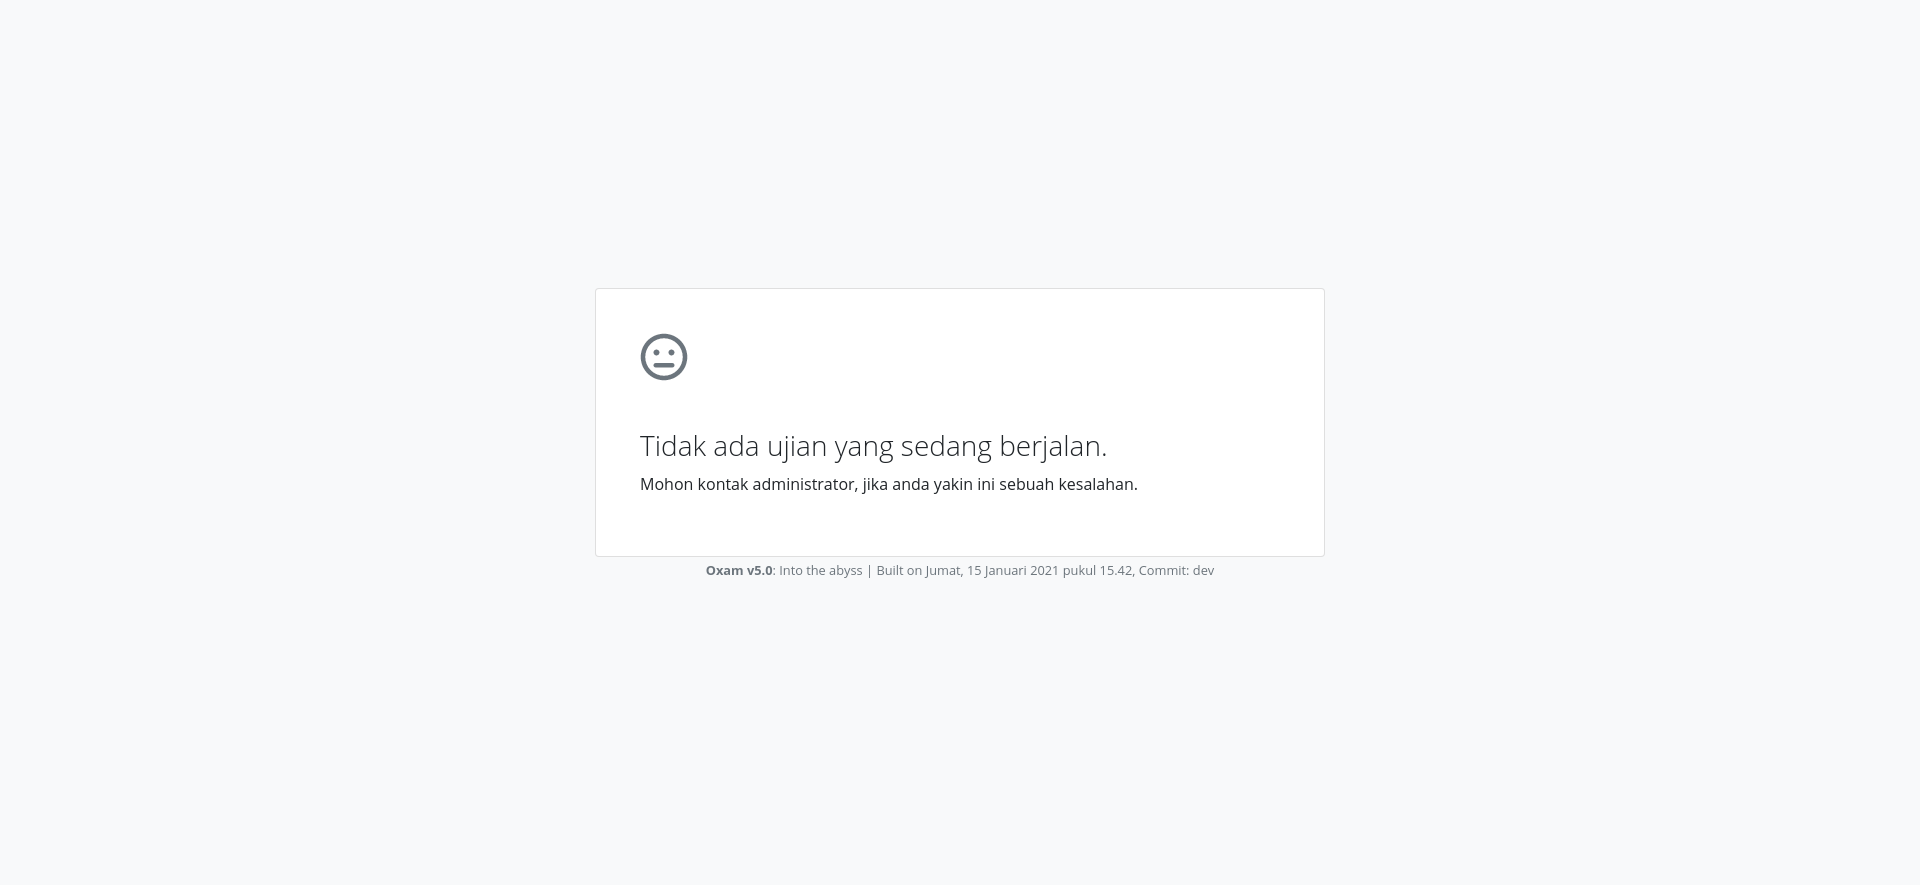
\includegraphics[width=0.7\paperwidth]{Gambar/implemented-interface/peserta/exam-empty.png}
            \caption{Tangkapan layar dari halaman ujian, dengan ujian yang tidak aktif.}
            \label{fig:screenshot-peserta-blankstate}
        \end{figure}
        
        \begin{figure}
            \centering
            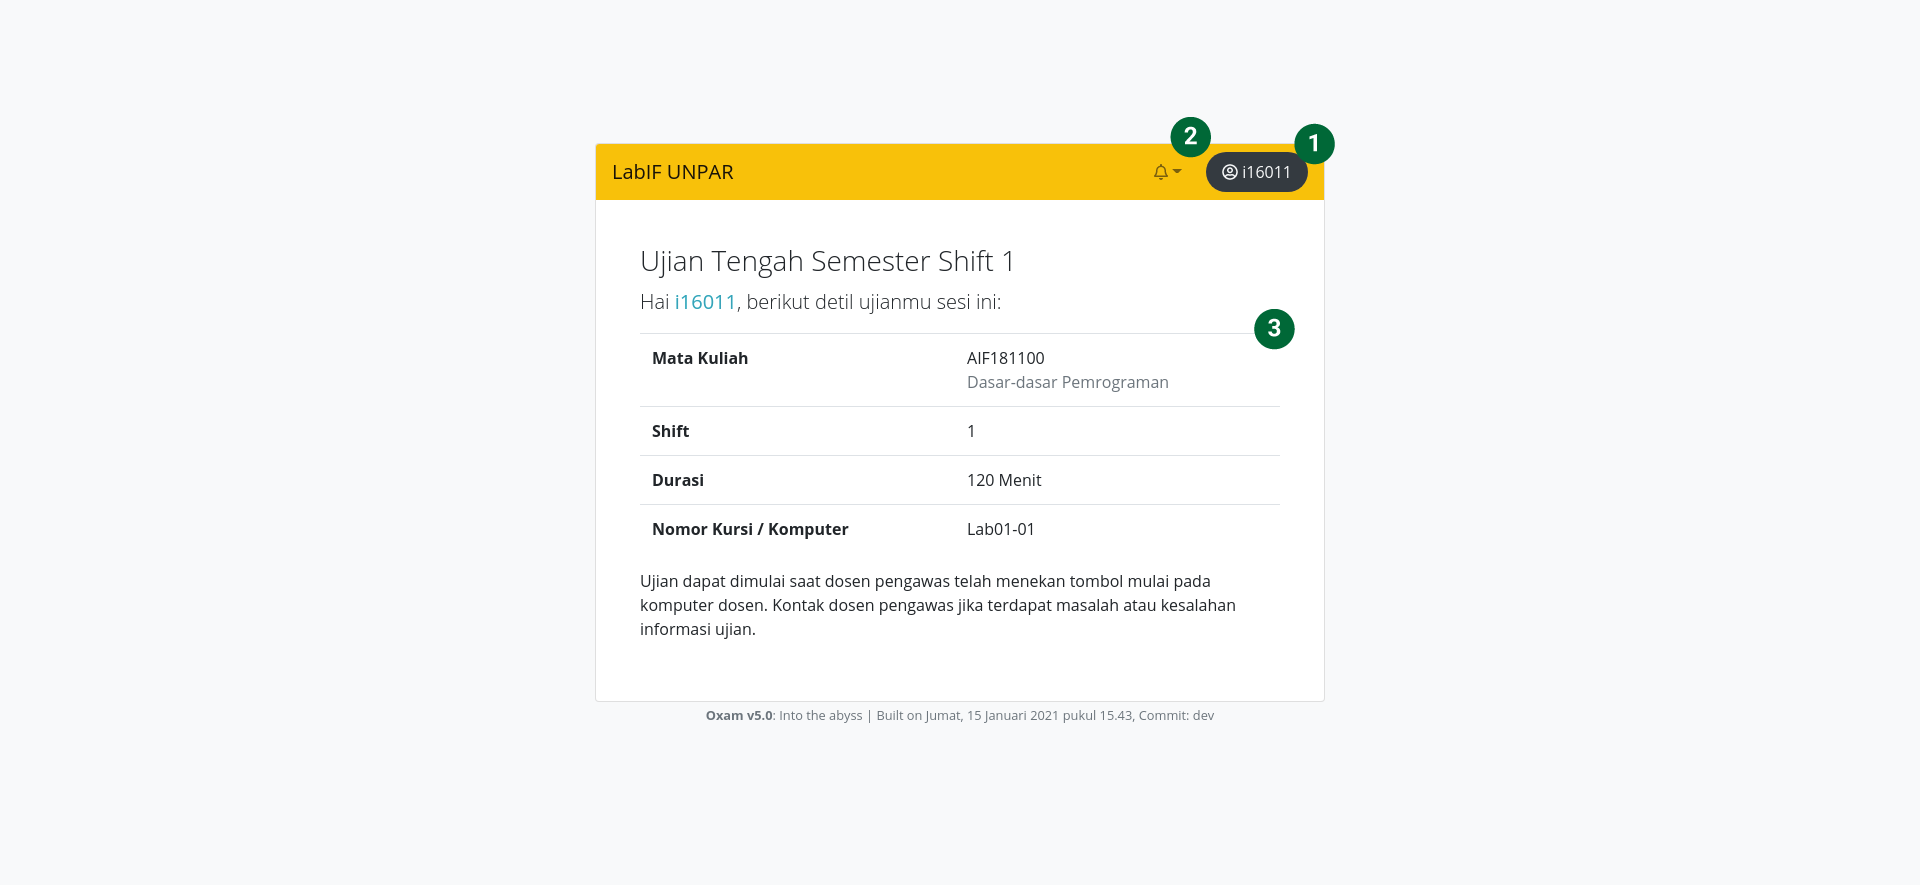
\includegraphics[width=0.7\paperwidth]{Gambar/implemented-interface/peserta/exam-standby.png}
            \caption{Tangkapan layar dari halaman ujian, dengan ujian yang akan aktif.}
            \label{fig:screenshot-peserta-standby}
        \end{figure}
        
        \begin{figure}
            \centering
            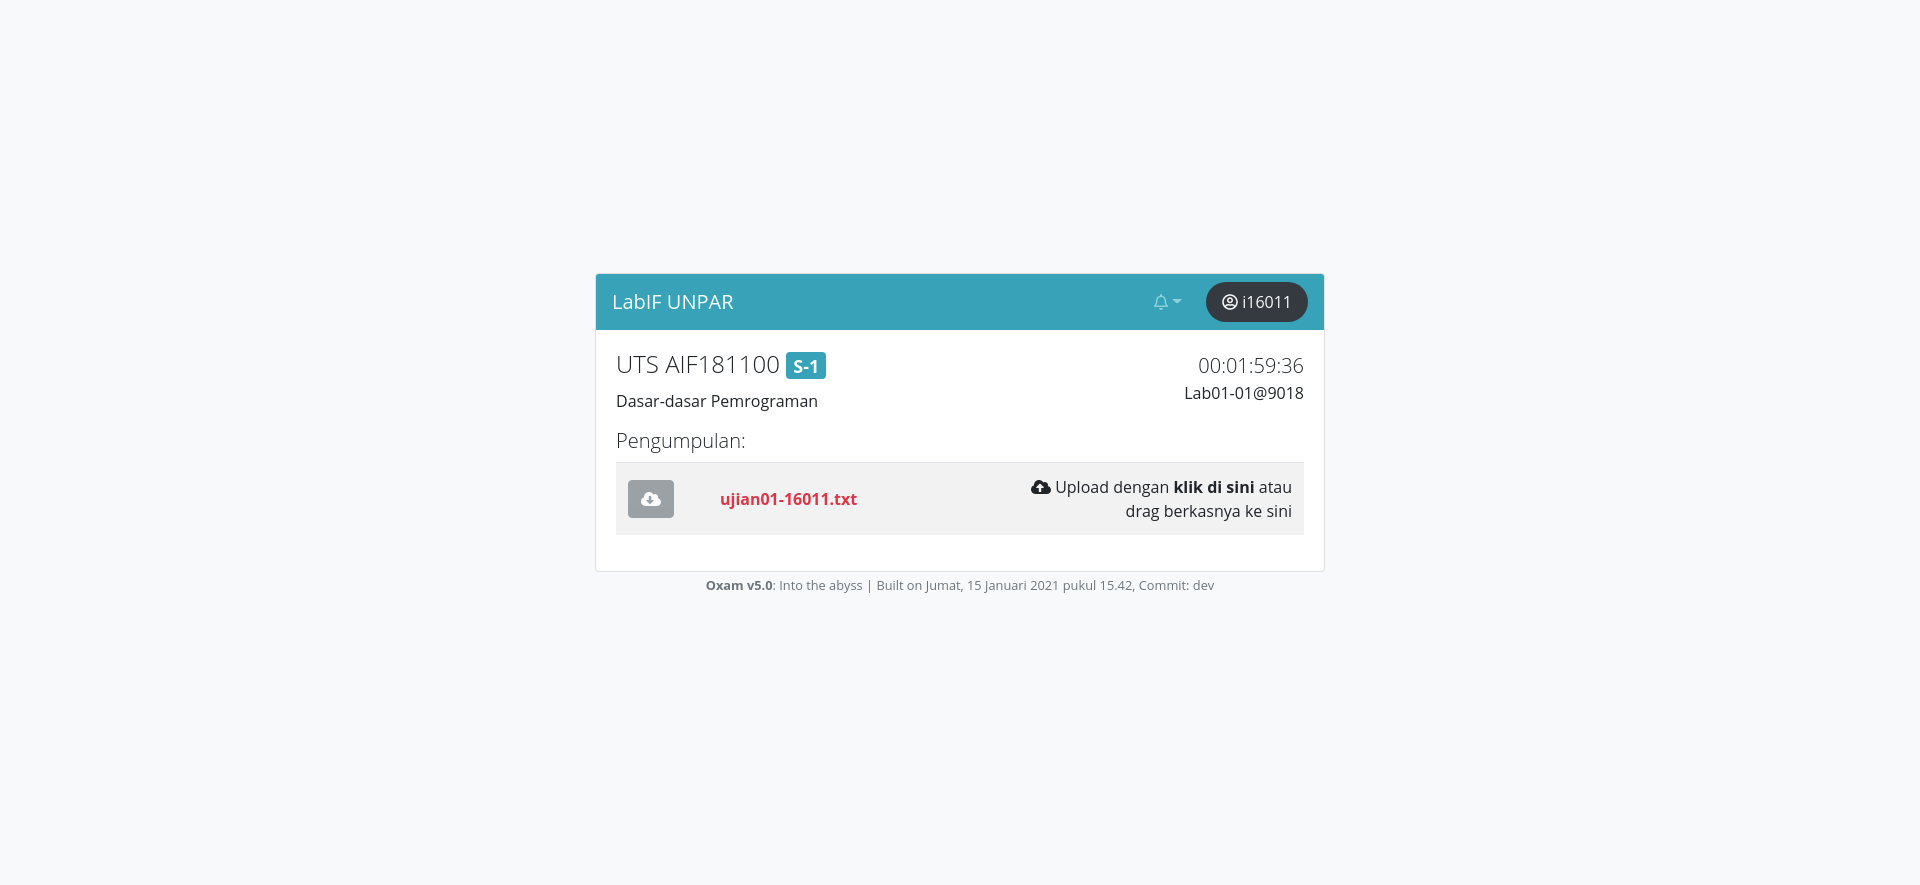
\includegraphics[width=0.7\paperwidth]{Gambar/implemented-interface/peserta/exam-open.png}
            \caption{Tangkapan layar dari halaman ujian, dengan ujian yang sedang aktif.}
            \label{fig:screenshot-peserta-open}
        \end{figure}
        
        \begin{figure}
            \centering
            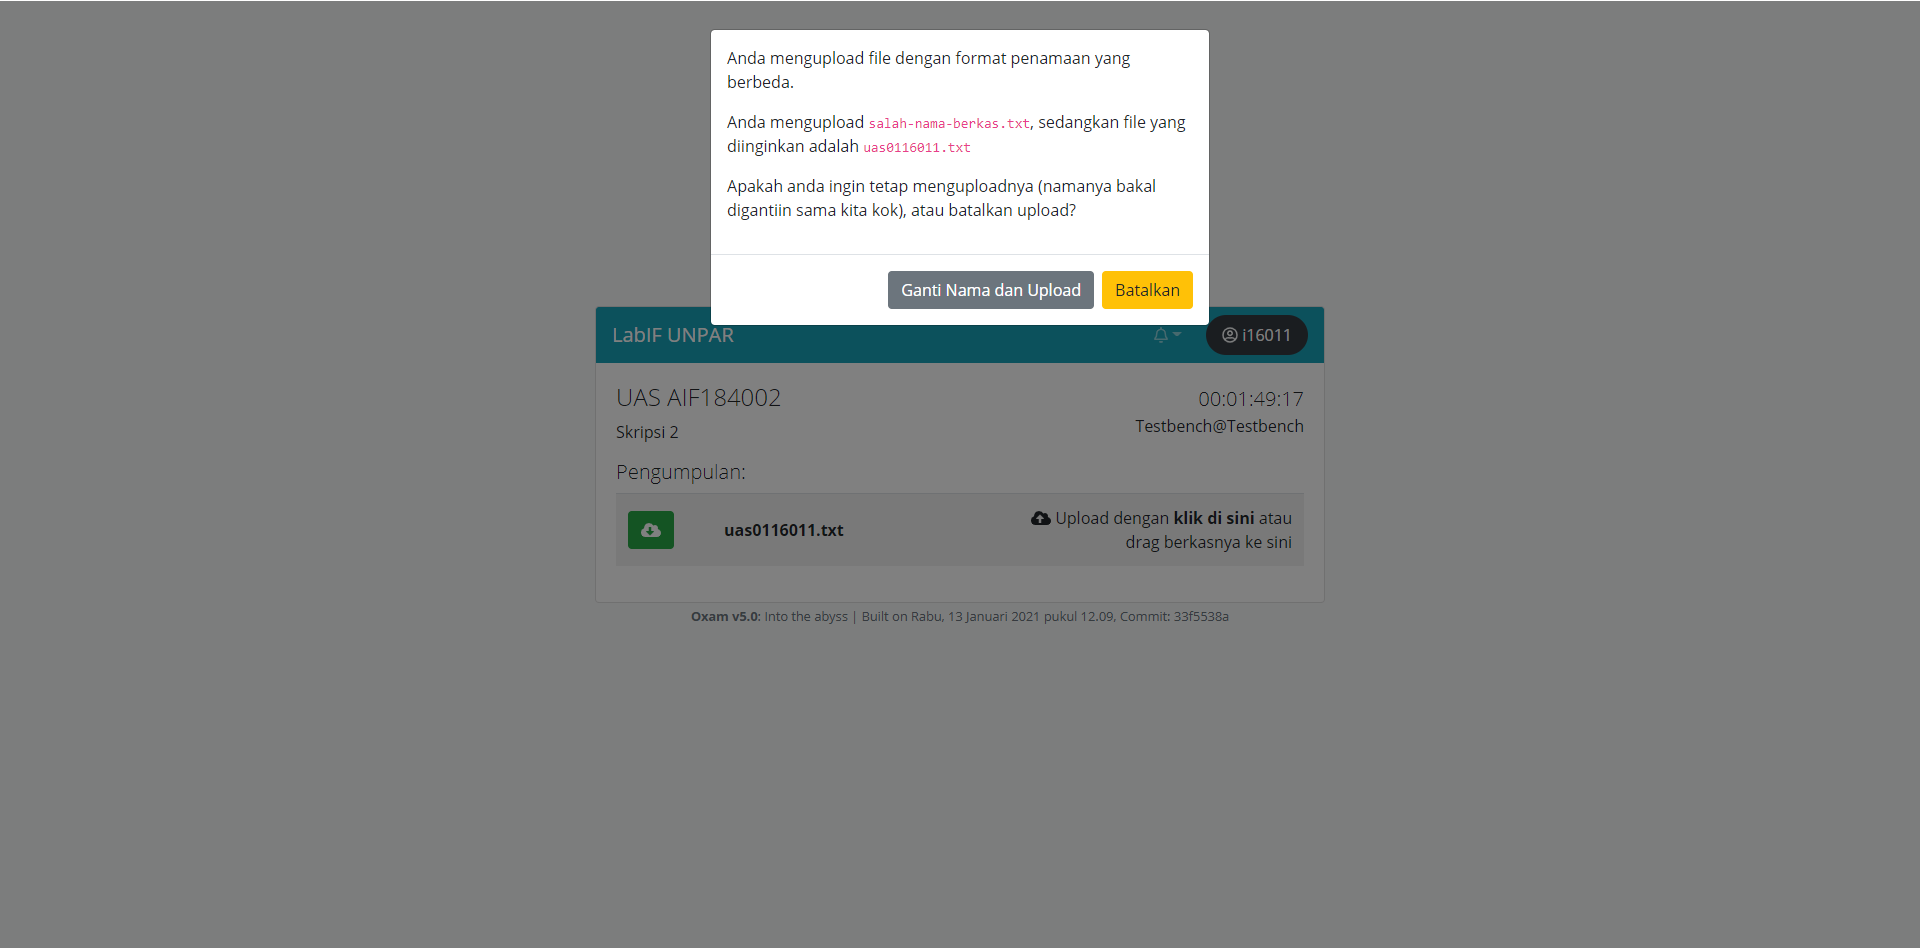
\includegraphics[width=0.7\paperwidth]{Gambar/implemented-interface/peserta/exam-wrong-filename.png}
            \caption{Tangkapan layar dari halaman ujian untuk peringatan nama berkas yang tidak sesuai.}
            \label{fig:screenshot-peserta-wrong-filename}
        \end{figure}
        
        \begin{figure}
            \centering
            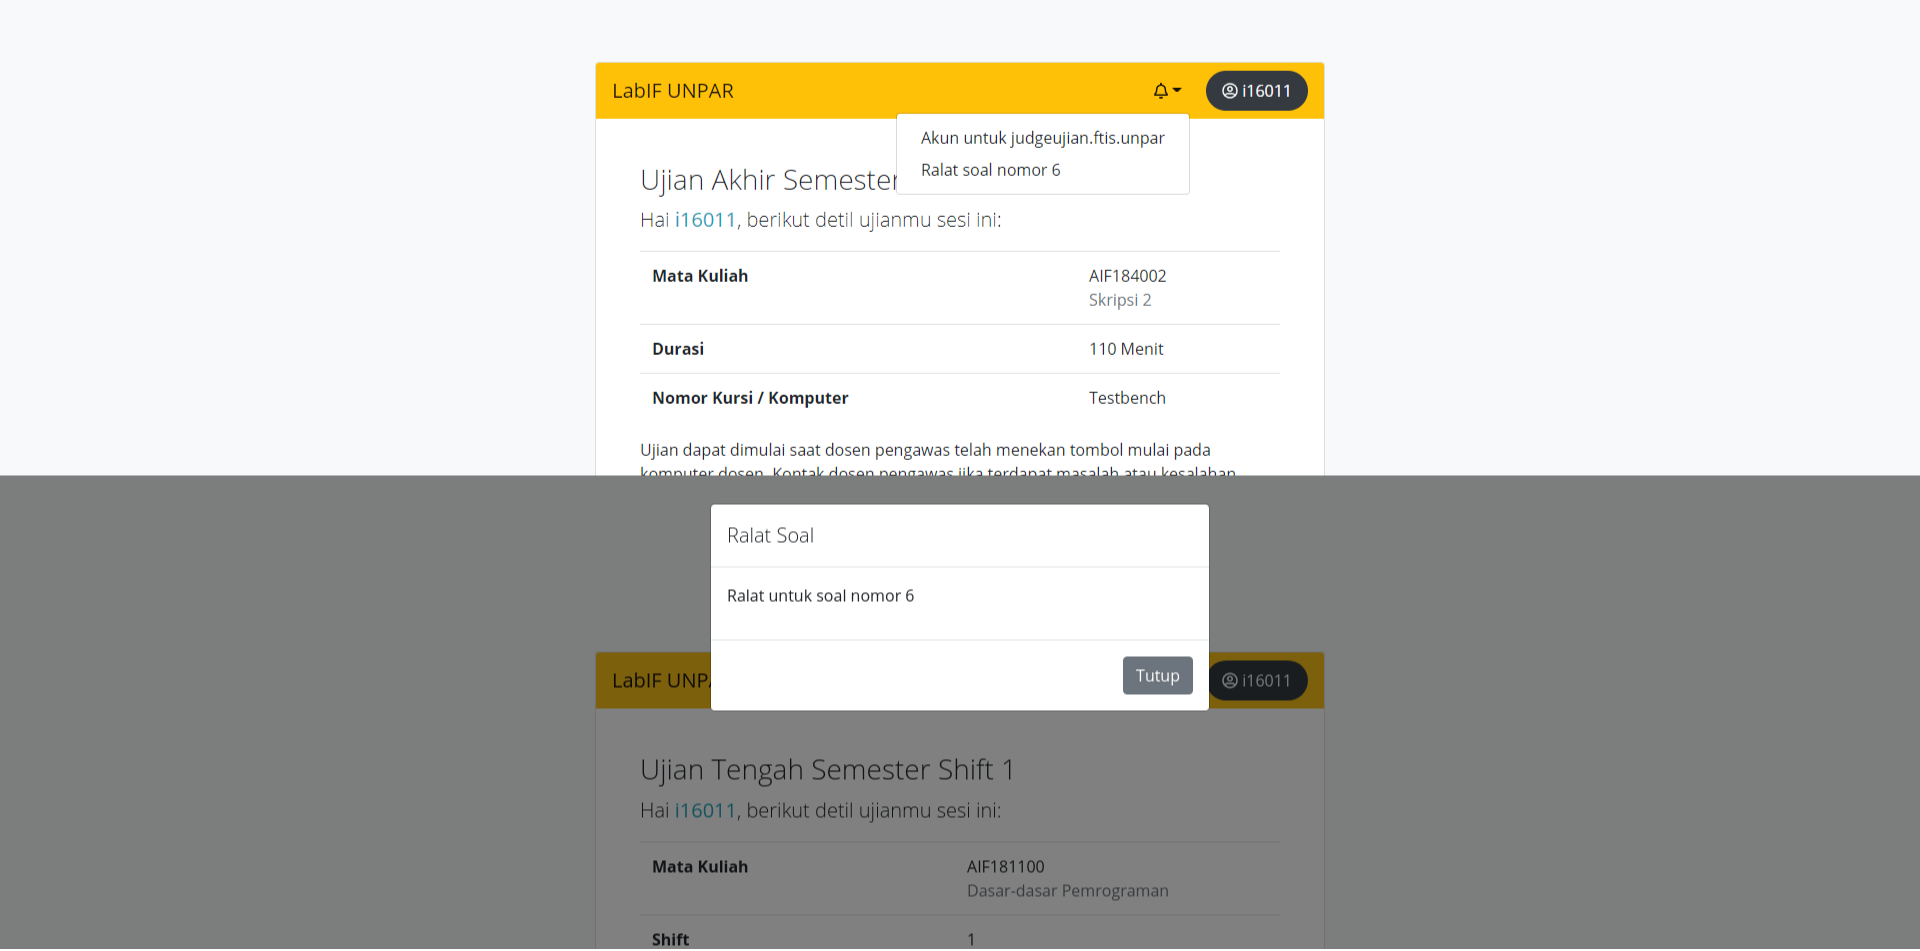
\includegraphics[width=0.7\paperwidth]{Gambar/implemented-interface/peserta/exam-notif.png}
            \caption{Tangkapan layar dari halaman ujian, bagian notifikasi.}
            \label{fig:screenshot-peserta-notification}
        \end{figure}
        
        Pada tangkapan layar halaman ujian yang tidak aktif (Gambar \ref{fig:screenshot-peserta-blankstate}), 
        peserta akan diberikan sebuah pesan
        yang memberitahukan bahwa tidak ada ujian yang aktif pada komputer tersebut. Selain itu, terdapat
        sebuah pesan status penting yang menandakan versi Oxam yang sedang aktif, dan jam terakhir
        \textit{build} pada subsistem frontend dibuat.
        
        Tangkapan layar halaman ujian yang akan aktif pada Gambar \ref{fig:screenshot-peserta-standby} menampilkan
        informasi penting tentang ujian yang akan aktif. Pada gambar tersebut, terdapat beberapa bagian yang ditunjuk
        oleh poin. Poin-poin tersebut terdiri dari
        \begin{itemize}
            \item Poin 1 menunjukkan informasi username peserta ujian.
            \item Poin 2 menunjukkan menu notifikasi.
            \item Poin 3 menunjukkan informasi ujian yang akan diadakan.
        \end{itemize}
        
        Tangakapan layar halaman ujian berikutnya adalah pada saat ujian sedang berjalan, dan lembar jawaban
        sedang dibuka. Tangkapan layar tersebut dapat dilihat pada Gambar \ref{fig:screenshot-peserta-open}.
        Bagian pada tangkapan layar tersebut terdiri dari:
        \begin{itemize}
            \item Poin 1 berisi informasi singkat tentang ujian yang aktif.
            \item Poin 2 adalah menu notifikasi dan informasi username peserta.
            \item Poin 3 menunjukkan waktu dan lokasi tempat duduk peserta.
            \item Poin 4 menunjukkan slot jawaban, tempat untuk mengunggah dan mengunduh berkas jawaban ujian
                yang ada pada ujian ini.
        \end{itemize}
        
        Jika peserta mengunggah berkas jawaban dengan nama berkas yang salah, peserta akan diberikan pesan peringatan untuk
        mengkonfirmasi perubahan nama berkas secara otomatis oleh sistem, tampilan tersebut dapat dilihat pada
        Gambar \ref{fig:screenshot-peserta-wrong-filename}.
        
        Tangkapan berikutnya adalah bagian bagian notifikasi. Tampilan tersebut dapat dilihat pada Gambar
        \ref{fig:screenshot-peserta-notification}. Bagian-bagian yang terdapat pada tangkapan layar tersebut
        terdiri dari:
        \begin{itemize}
            \item Poin 1 menunjukkan menu notifikasi yang tersedia.
            \item Poin 2 menunjukkan notifikasi yang sedang dibuka.
        \end{itemize}
        
    \subsection{Halaman untuk Tim Admin}
    Halaman untuk Tim Admin memiliki beberapa bagian besar yang akan dipisah berdasarkan fungsi utamanya.
    Kelompok pertama yang akan dibahas adalah bagian otentikasi. Kemudian pembahasan akan maju ke bagian
    ujian, lalu yang terakhir editor entitas.
    
    \subsubsection{Halaman Otentikasi}
    \begin{figure}
        \centering
        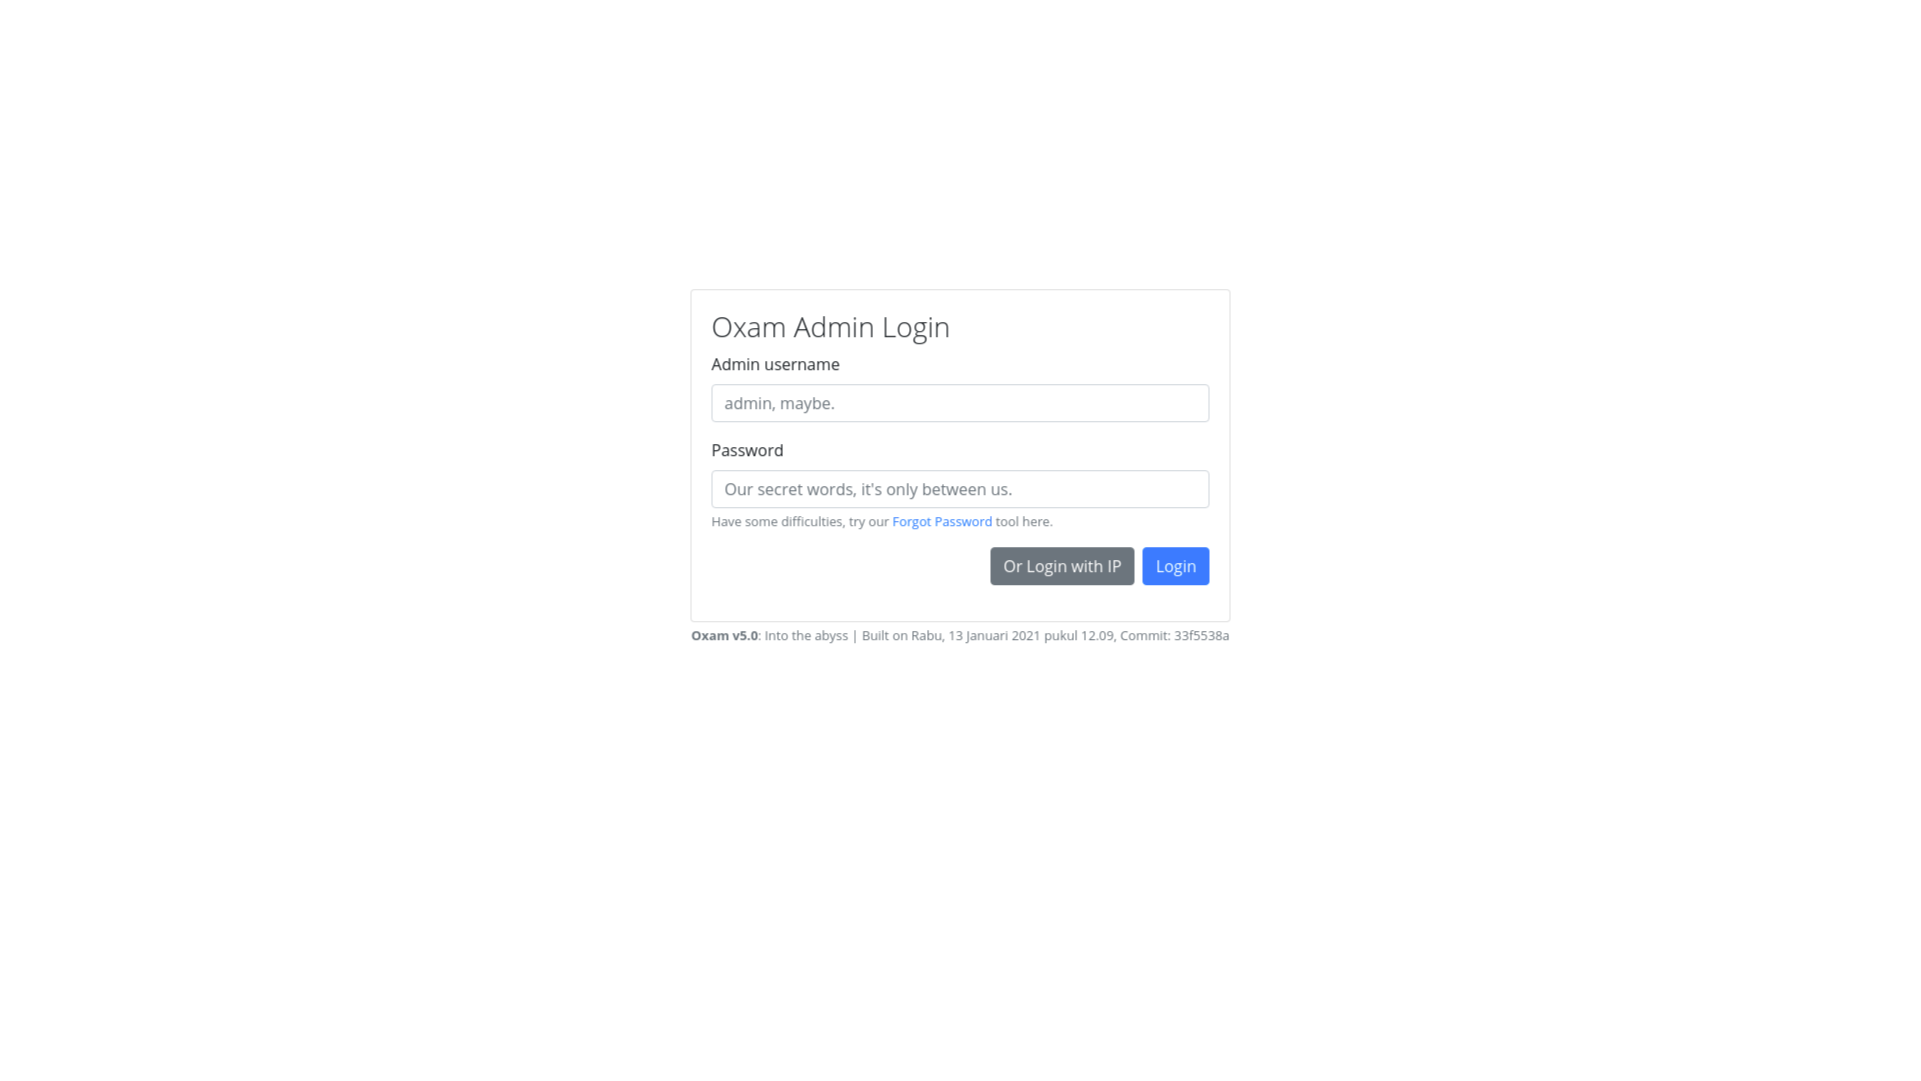
\includegraphics[width=0.7\paperwidth]{Gambar/implemented-interface/admin/login.png}
        \caption{Tangkapan layar halaman otentikasi}
        \label{fig:screenshot-admin-authentication}
    \end{figure}
    Implementasi halaman otentikasi dapat dilihat pada Gambar \ref{fig:screenshot-admin-authentication}. Pada
    gambar tersebut terdapat bagian-bagian yang terdiri dari
    \begin{itemize}
        \item Poin 1 bidang username.
        \item Poin 2 bidang kata sandi.
        \item Poin 3 tombol untuk login dengan IPLogin.
        \item Poin 4 tombol untuk login dengan kredensial biasa.
    \end{itemize}
    
    \subsubsection{Halaman untuk Ujian}
    \begin{figure}
        \centering
        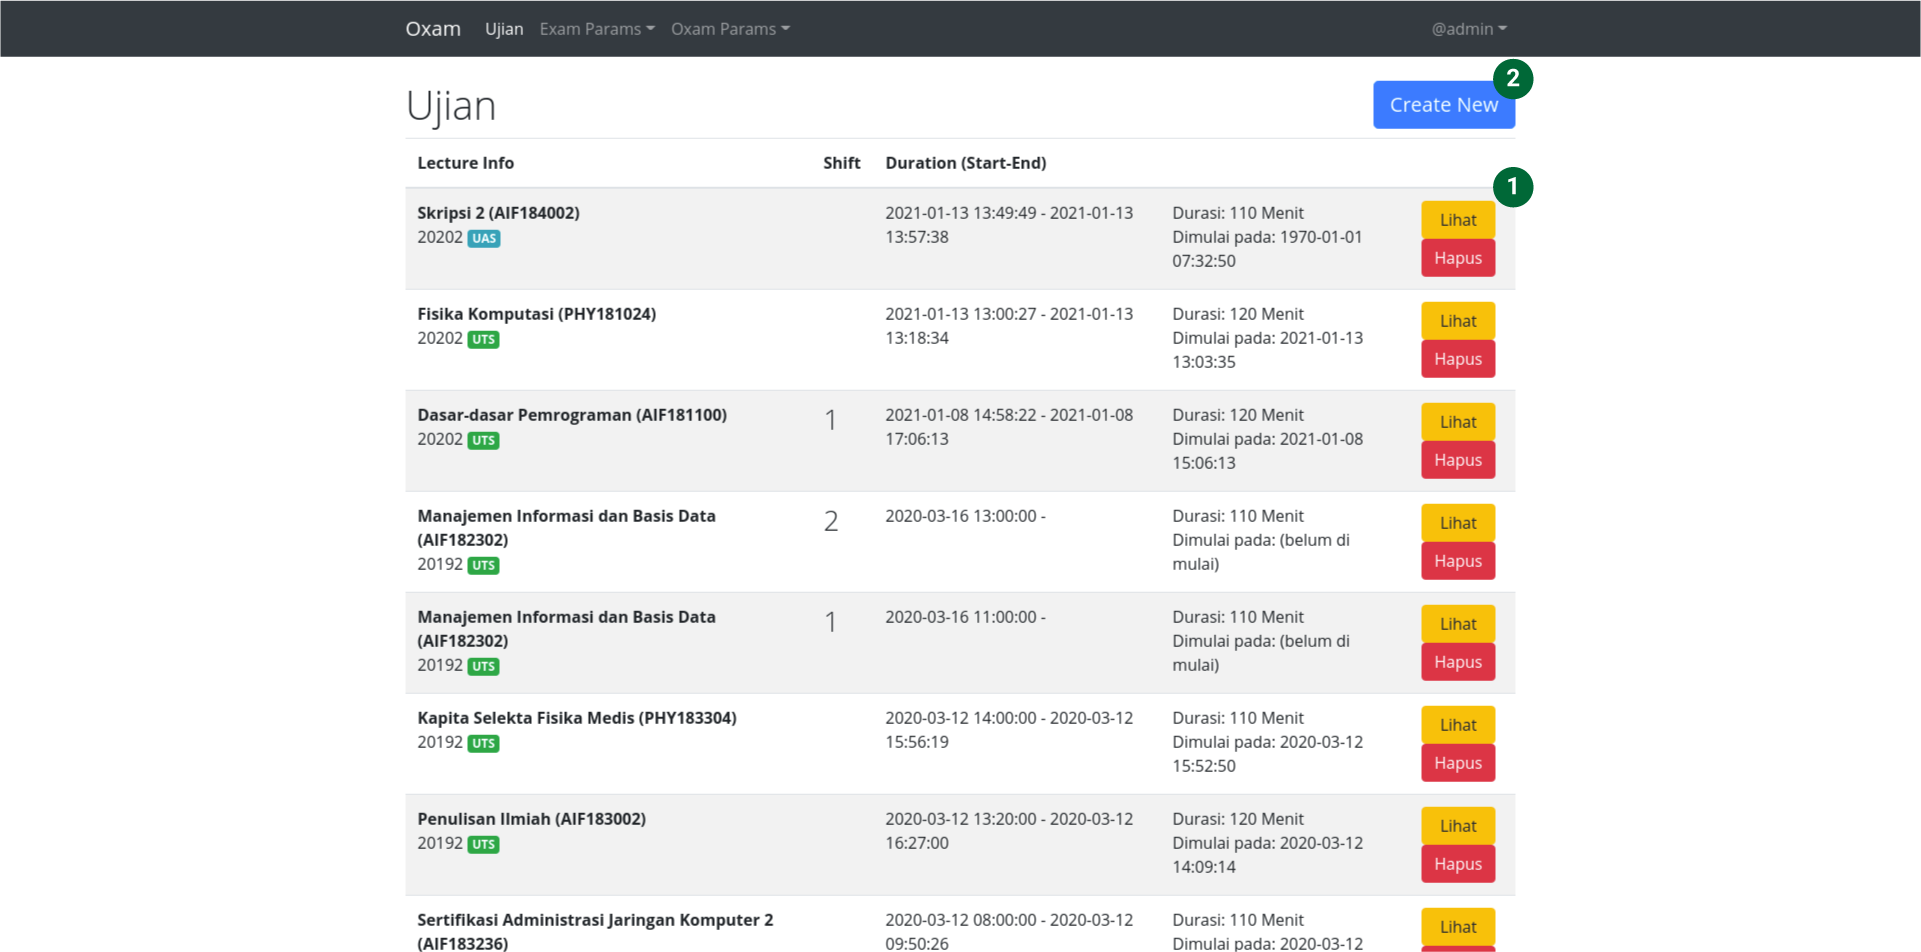
\includegraphics[width=0.7\paperwidth]{Gambar/implemented-interface/admin/ujian-list.png}
        \caption{Tangkapan layar daftar ujian untuk admin.}
        \label{fig:screenshot-admin-exam-list}
    \end{figure}
    Tangkapan layar untuk ujian pertama adalah halaman daftar ujian, dapat dilihat pada gambar
    \ref{fig:screenshot-admin-exam-list}. Bagian yang ditujukkan pada gambar tersebut teridiri dari
    \begin{itemize}
        \item Poin 1 menunjukkan informasi ujian pada entri, tombol untuk melihat ujian tersebut, serta
            tombol untuk menghapus ujian tersebut.
        \item Poin 2 menunjukkan tombol pembuatan ujian baru.
    \end{itemize}
    
    \begin{figure}
        \centering
        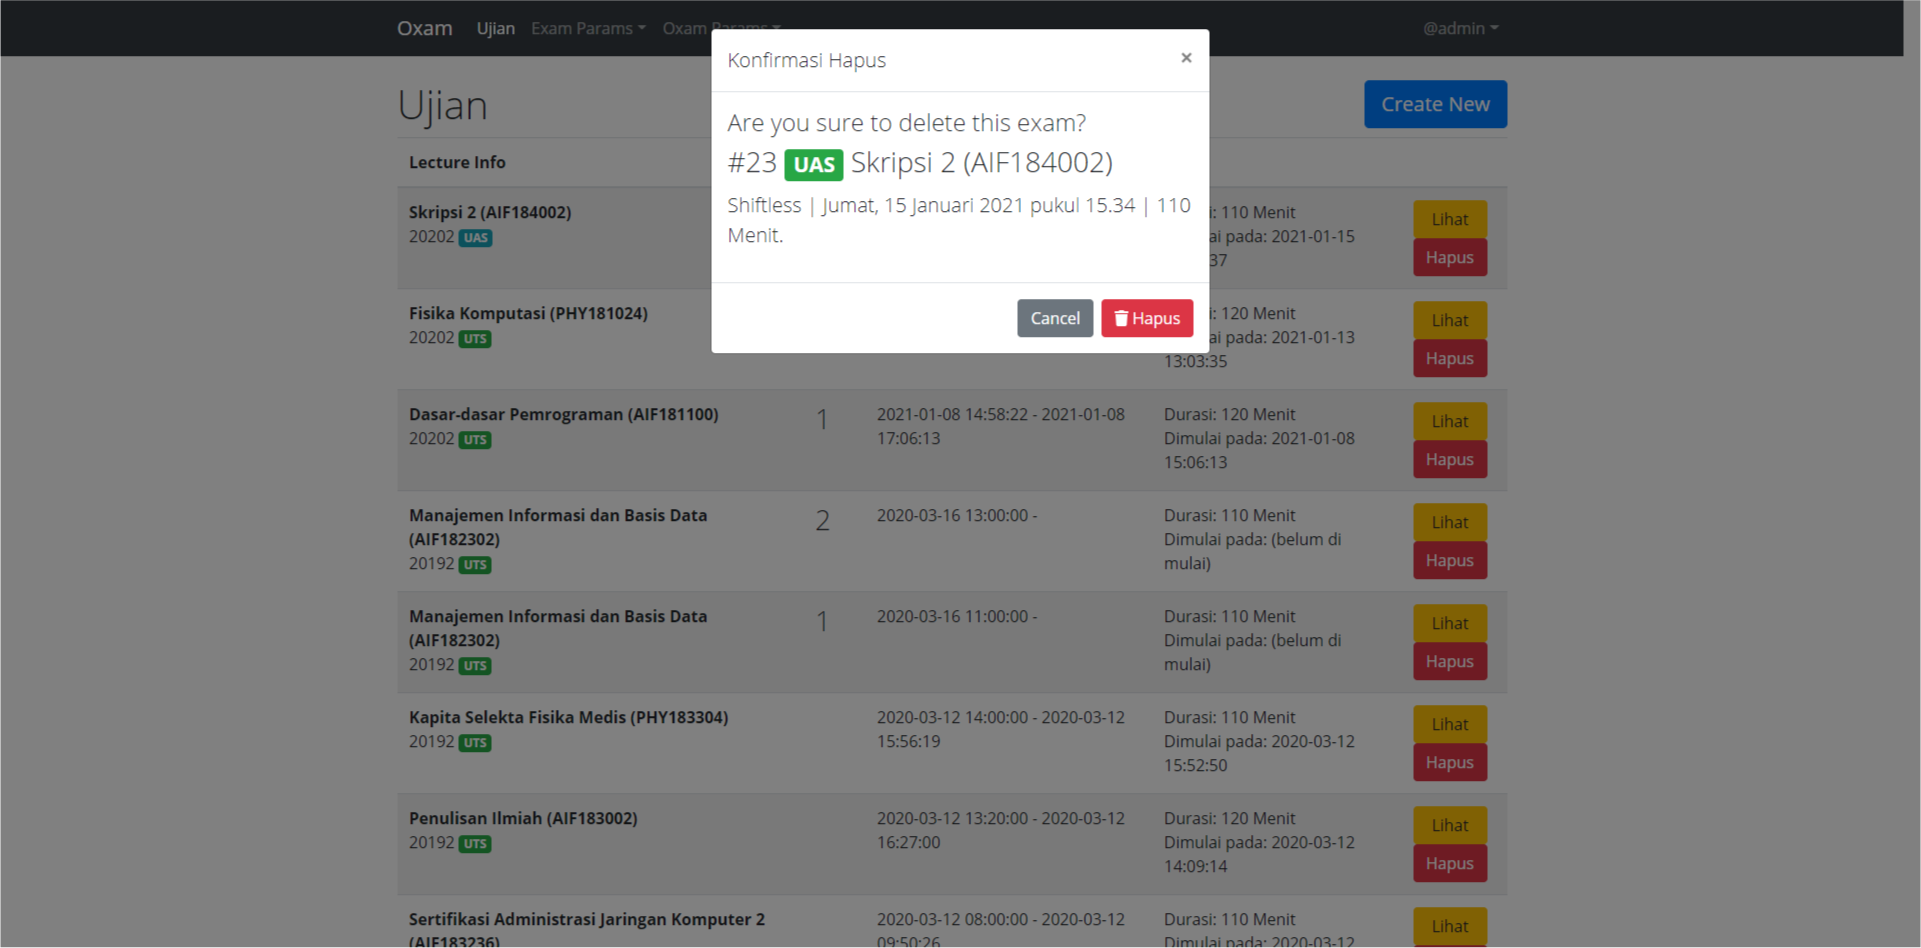
\includegraphics[width=0.7\paperwidth]{Gambar/implemented-interface/admin/ujian-delete.png}
        \caption{Tangkapan layar konfirmasi penghapusan ujian.}
        \label{fig:screenshot-admin-exam-delete}
    \end{figure}
    Tampilan konfirmasi penghapusan ujian dapat dilihat pada Gambar \ref{fig:screenshot-admin-exam-delete}.
    Tampilan tersebut terdiri dari informasi singkat tentang ujian dan tombol konfirmasi penghapusan
    dan pembatalan.
    
    \begin{figure}
        \centering
        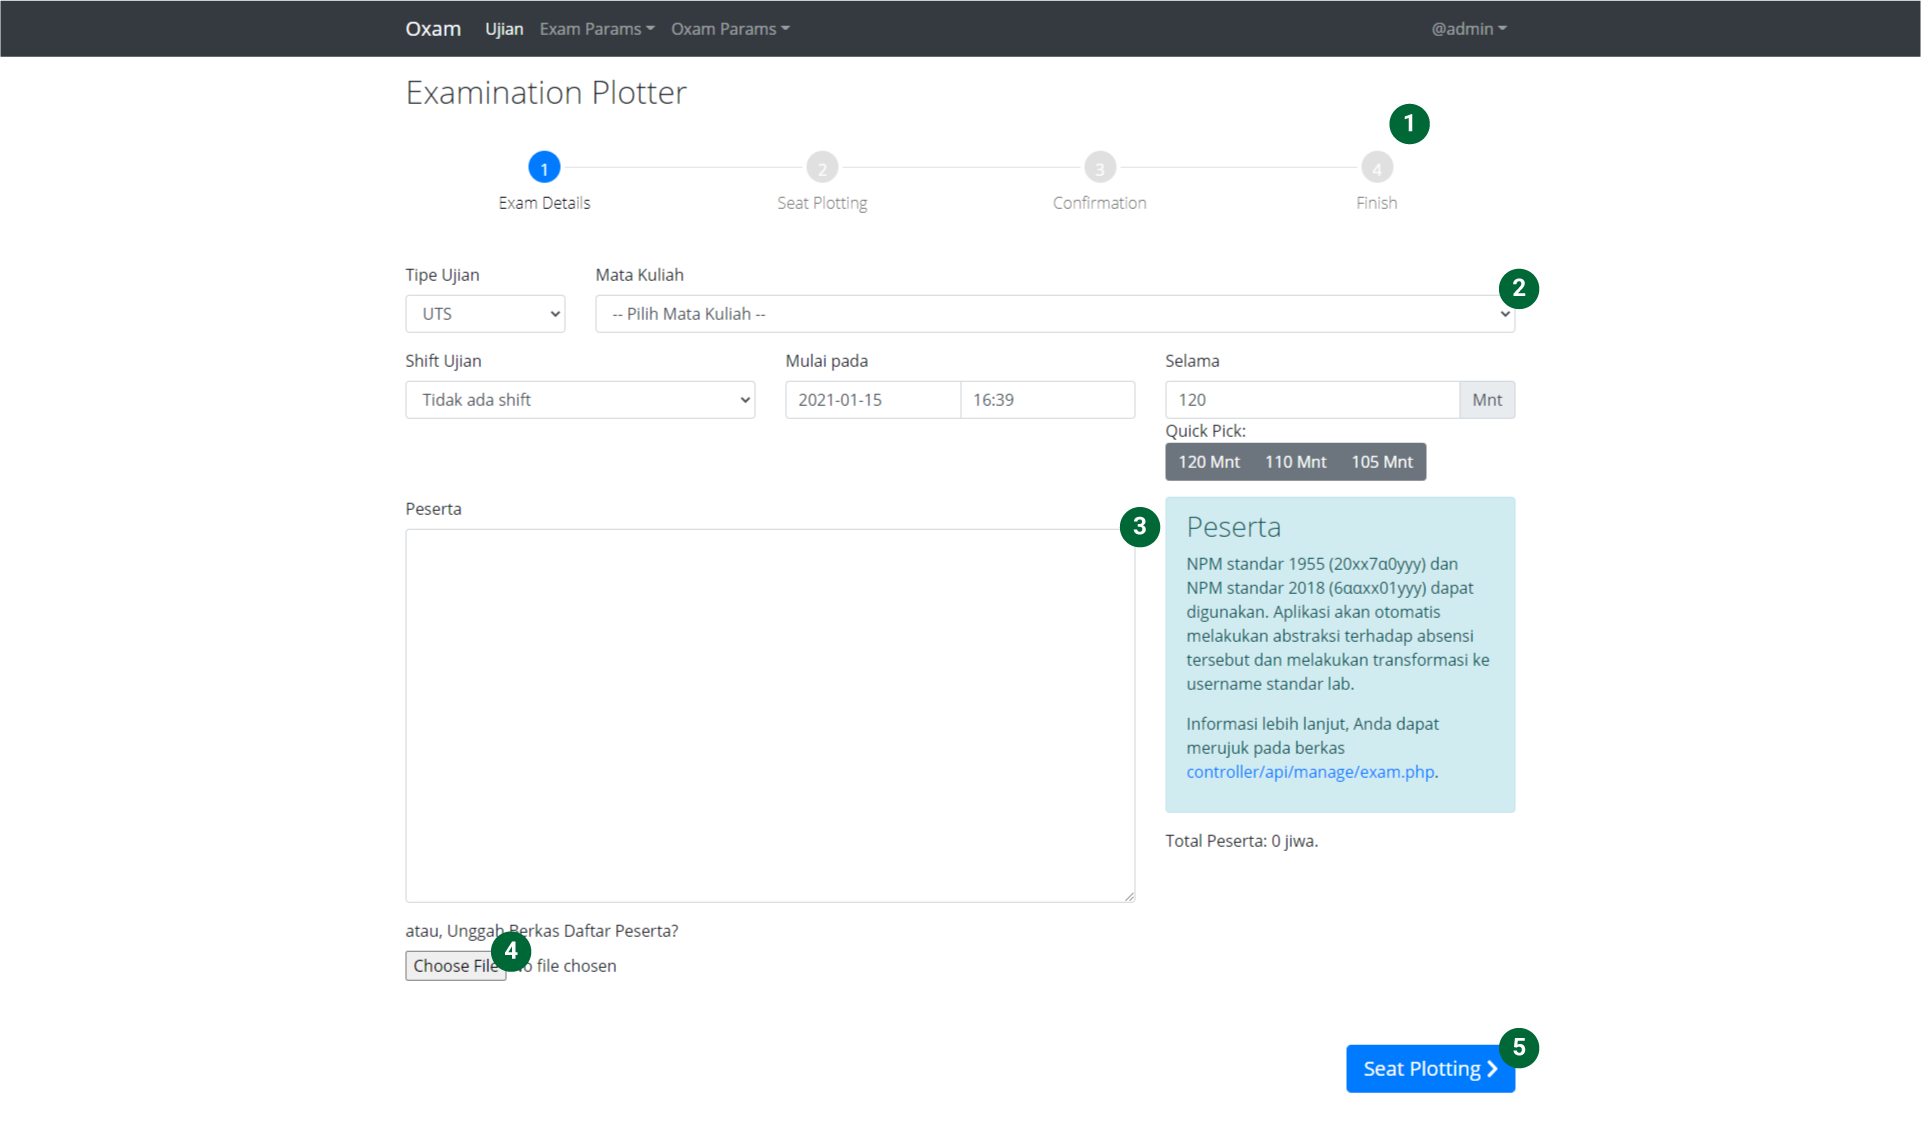
\includegraphics[width=0.7\paperwidth]{Gambar/implemented-interface/admin/ujian-make-1.png}
        \caption{Tangkapan layar untuk membuat ujian, langkah pertama.}
        \label{fig:screenshot-admin-exam-make-1}
    \end{figure}\begin{figure}
        \centering
        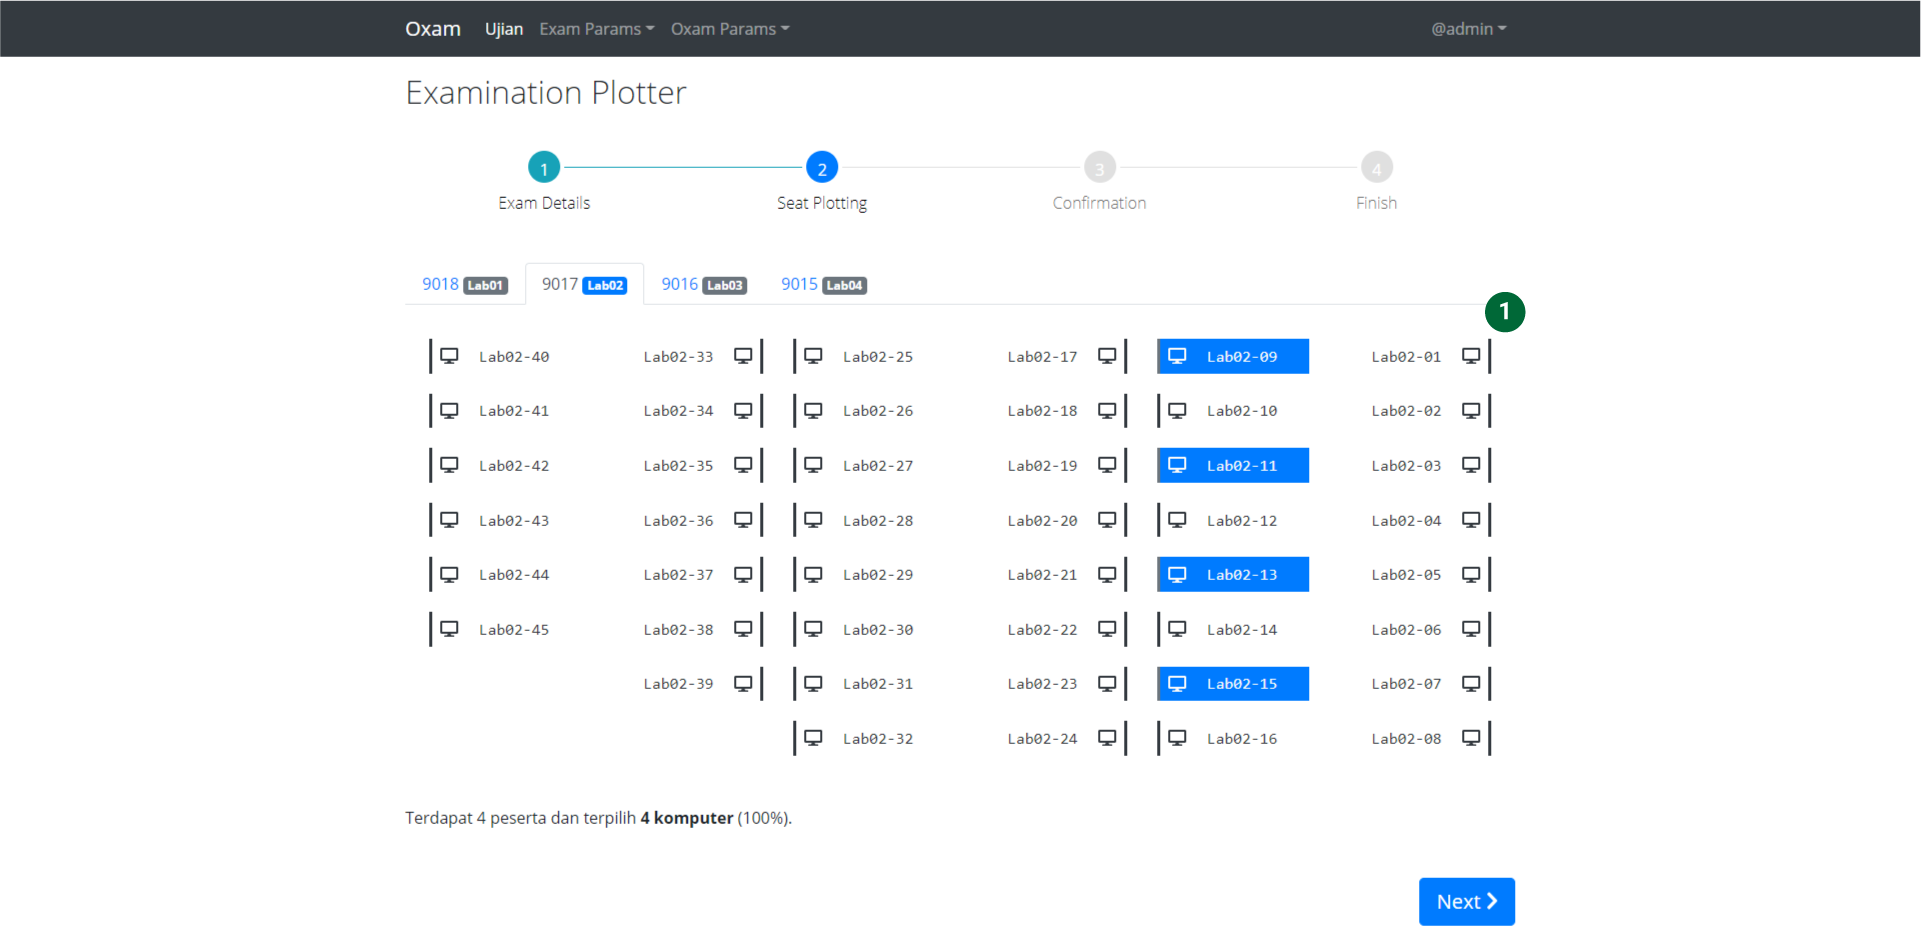
\includegraphics[width=0.7\paperwidth]{Gambar/implemented-interface/admin/ujian-make-2.png}
        \caption{Tangkapan layar untuk membuat ujian, langkah kedua.}
        \label{fig:screenshot-admin-exam-make-2}
    \end{figure}\begin{figure}
        \centering
        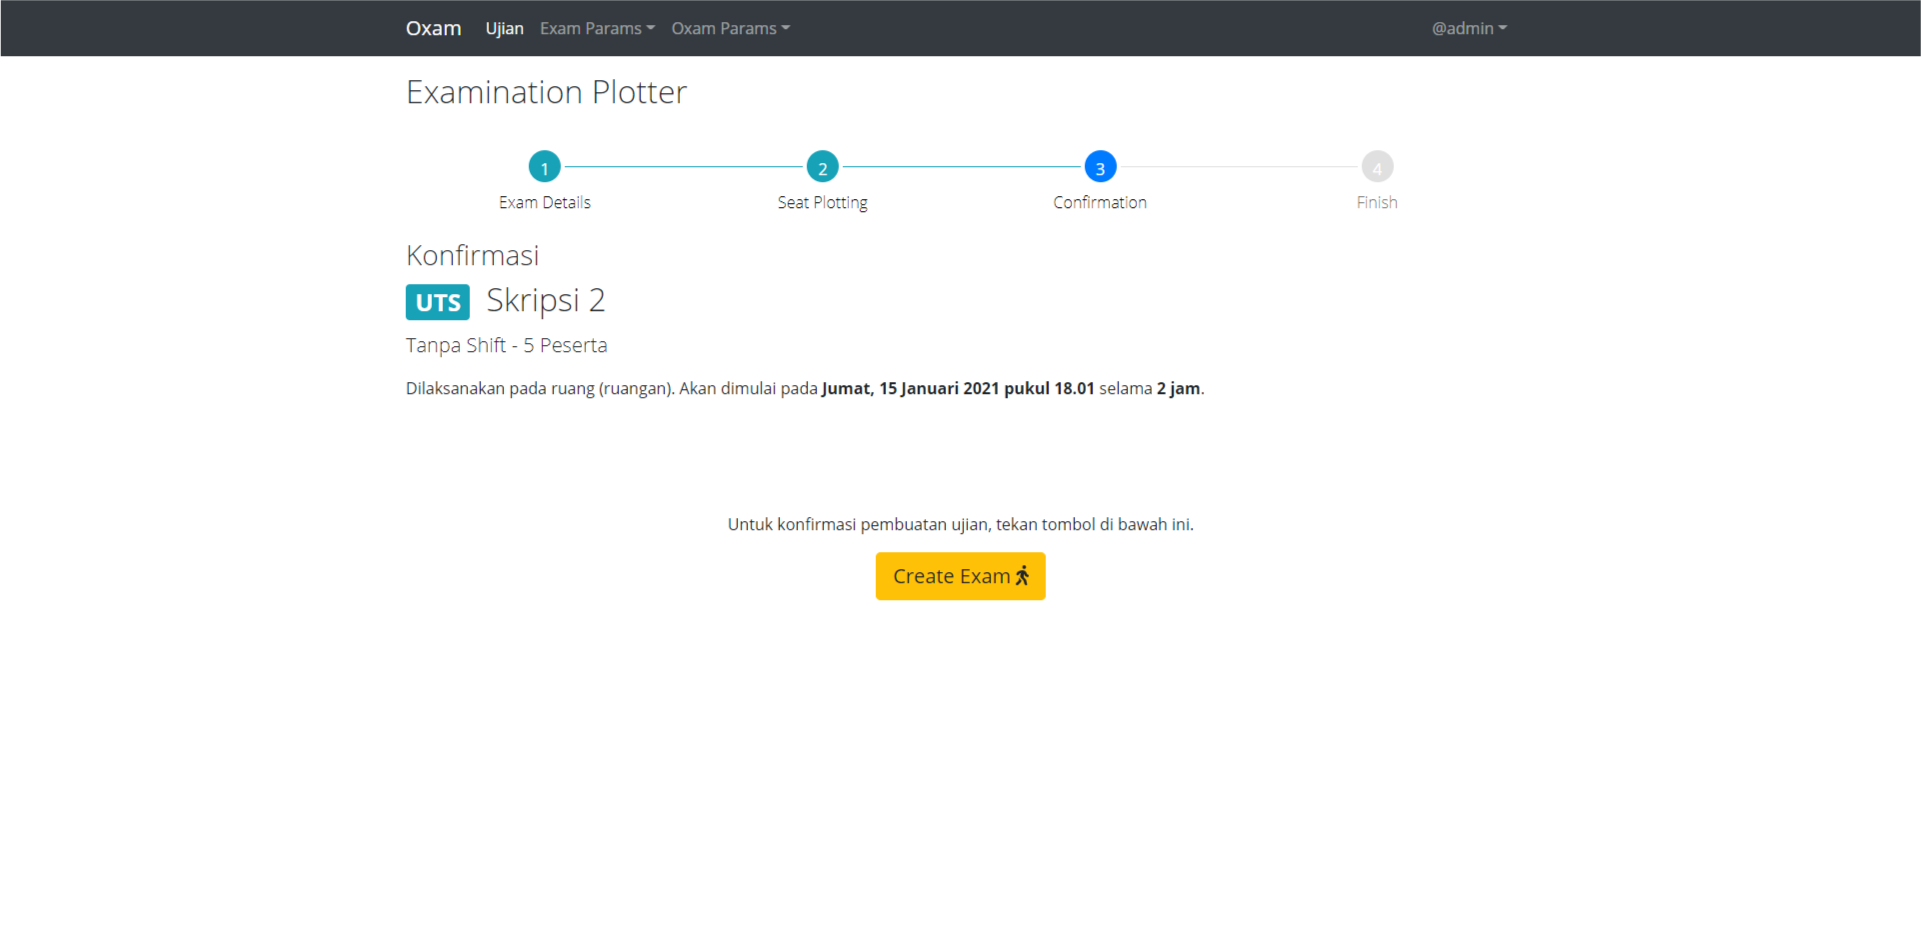
\includegraphics[width=0.7\paperwidth]{Gambar/implemented-interface/admin/ujian-make-3.png}
        \caption{Tangkapan layar untuk membuat ujian, langkah ketiga.}
        \label{fig:screenshot-admin-exam-make-3}
    \end{figure}\begin{figure}
        \centering
        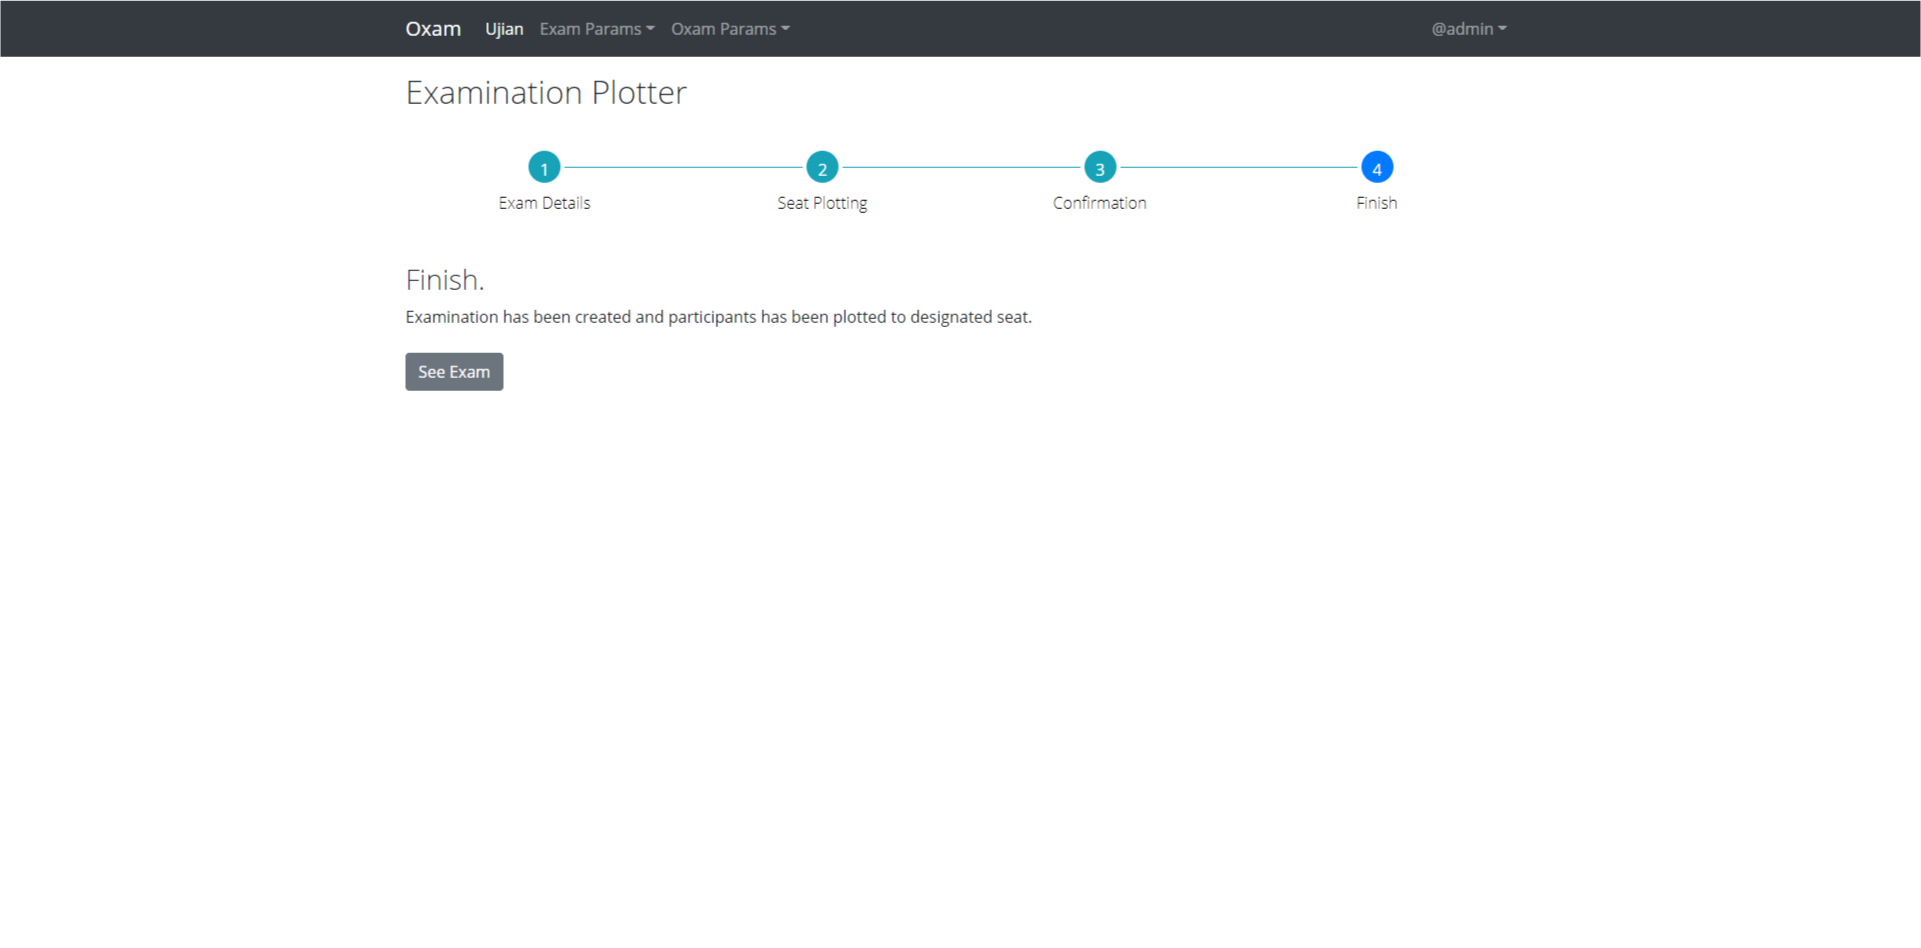
\includegraphics[width=0.7\paperwidth]{Gambar/implemented-interface/admin/ujian-make-4.png}
        \caption{Tangkapan layar untuk membuat ujian, langkah keempat.}
        \label{fig:screenshot-admin-exam-make-4}
    \end{figure}
    Tampilan berikutnya adalah tampilan untuk membuat ujian baru, tampilan tersebut dapat dilihat
    pada Gambar \ref{fig:screenshot-admin-exam-make-1}, \ref{fig:screenshot-admin-exam-make-2},
    \ref{fig:screenshot-admin-exam-make-3}, dan \ref{fig:screenshot-admin-exam-make-4}. Bagian
    yang ditunjukkan pada Gambar \ref{fig:screenshot-admin-exam-make-1} terdiri dari
    \begin{itemize}
        \item Poin 1 berisi informasi langkah yang saat ini sedang aktif.
        \item Poin 2 adalah formulir detil ujian.
        \item Poin 3 adalah daftar peserta, yang juga dapat diunggah dengan menggunakan file pada;
        \item Poin 4 menunjukkan bidang pengunggahan berkas daftar peserta.
    \end{itemize}
    Tangkapan layar langkah kedua pada Gambar \ref{fig:screenshot-admin-exam-make-2} terdiri dari
    \begin{itemize}
        \item Poin 1 berisi daftar peta tempat duduk peserta pada setiap ruangan.
    \end{itemize}
    Sedangkan pada langkah ketiga yang dapat dilihat pada Gambar \ref{fig:screenshot-admin-exam-make-3},
    terdiri dari
    \begin{itemize}
        \item Poin 1 berisi informasi singkat tentang ujian yang akan dibuat.
        \item Poin 2 tombol konfirmasi pembuatan ujian.
    \end{itemize}
    Lalu, pada langkah terakhir yang dapat dilihat pada Gambar \ref{fig:screenshot-admin-exam-make-4},
    tangkapan layar hanya akan menunjukkan konfirmasi ujian telah berhasil dibuat dan pengguna
    diberikan sebuah tombol navigasi untuk melihat ujian.
    
    \begin{figure}
        \centering
        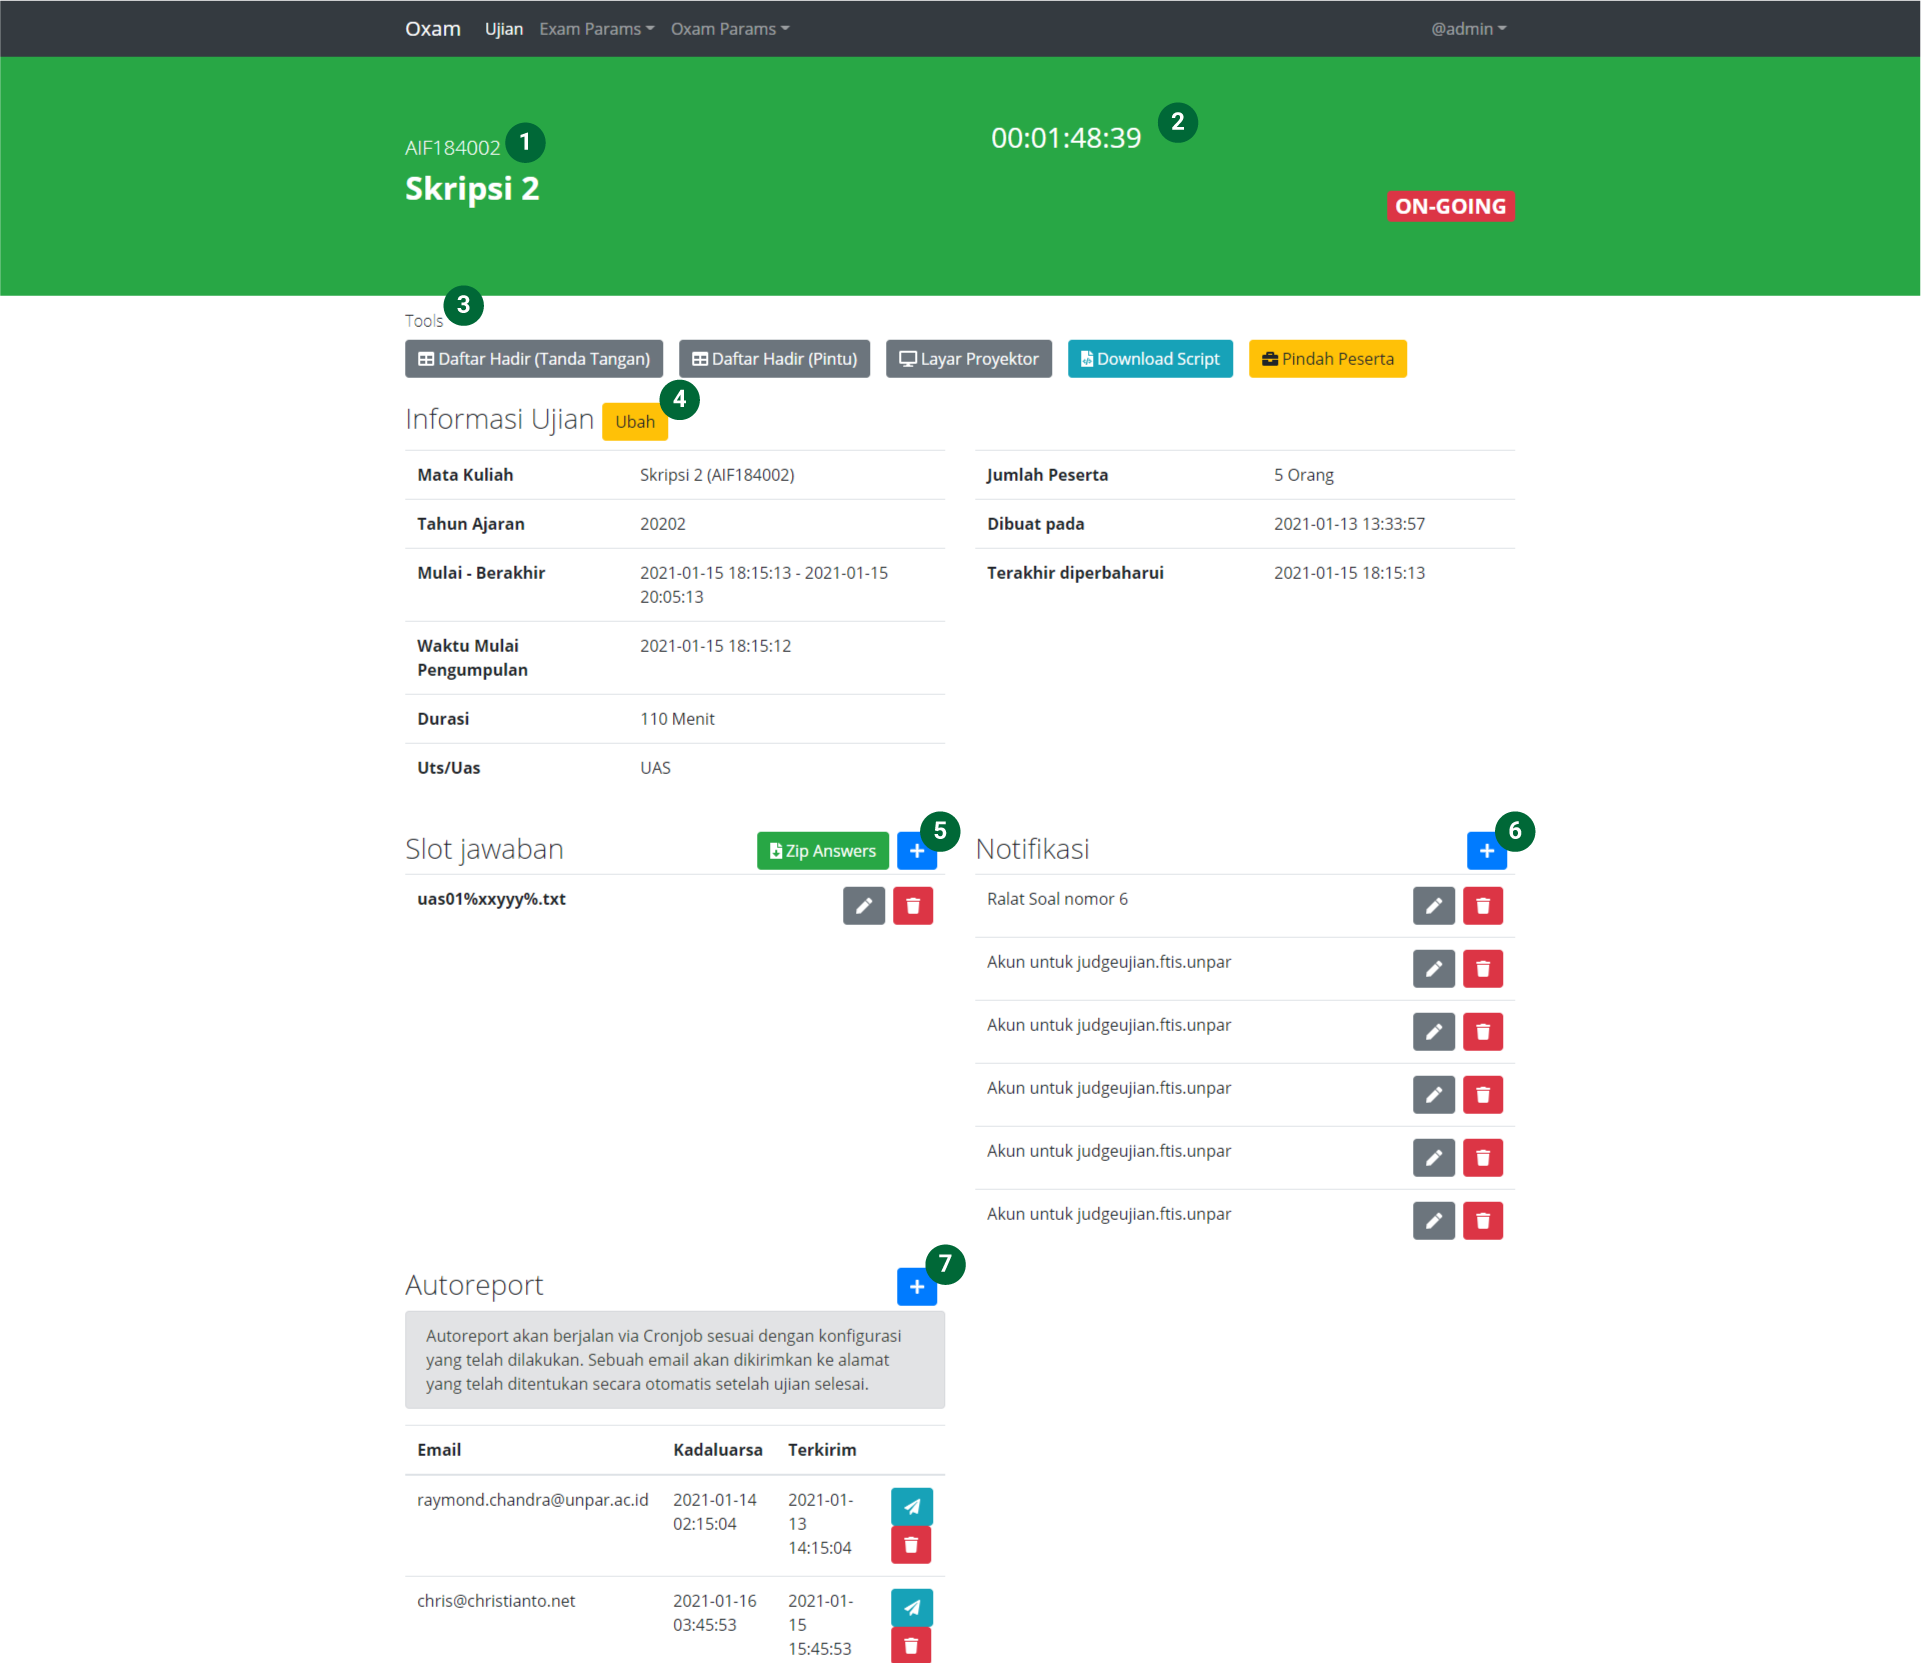
\includegraphics[width=0.7\paperwidth]{Gambar/implemented-interface/admin/ujian-detail.png}
        \caption{Tangkapan layar untuk detil ujian}
        \label{fig:screenshot-admin-exam-detail}
    \end{figure}
    Halaman detil ujian akan memiliki beberapa tombol peralatan yang dapat dilihat pada Gambar
    \ref{fig:screenshot-admin-exam-detail}. Poin yang terlihat pada gambar tersebut terdiri dari
    \begin{itemize}
        \item Poin 1 menunjukkan informasi singkat tentang ujian.
        \item Poin 2 status singkat tentang ujian, sedang dimulai dan waktu yang tersisa.
        \item Poin 3 menunjukkan tombol-tombol peralatan yang dapat digunakan oleh Tim Admin, yang
            teridiri dari
            \begin{itemize}
                \item Daftar Hadir untuk tanda tangan.
                \item Daftar Hadir untuk ditempelkan pada pintu.
                \item Layar Proyektor.
                \item Unduh \textit{script}.
                \item Pindah Peserta.
            \end{itemize}
        \item Poin 4 informasi singkat ujian dengan tombol pengubahnya.
        \item Poin 5 menunjukkan fitur slot jawaban.
        \item Poin 6 menunjukkan fitur notifikasi
        \item Poin 7 menunjukkan fitur pelaporan otomatis.
    \end{itemize}
    
    
    \begin{figure}
        \centering
        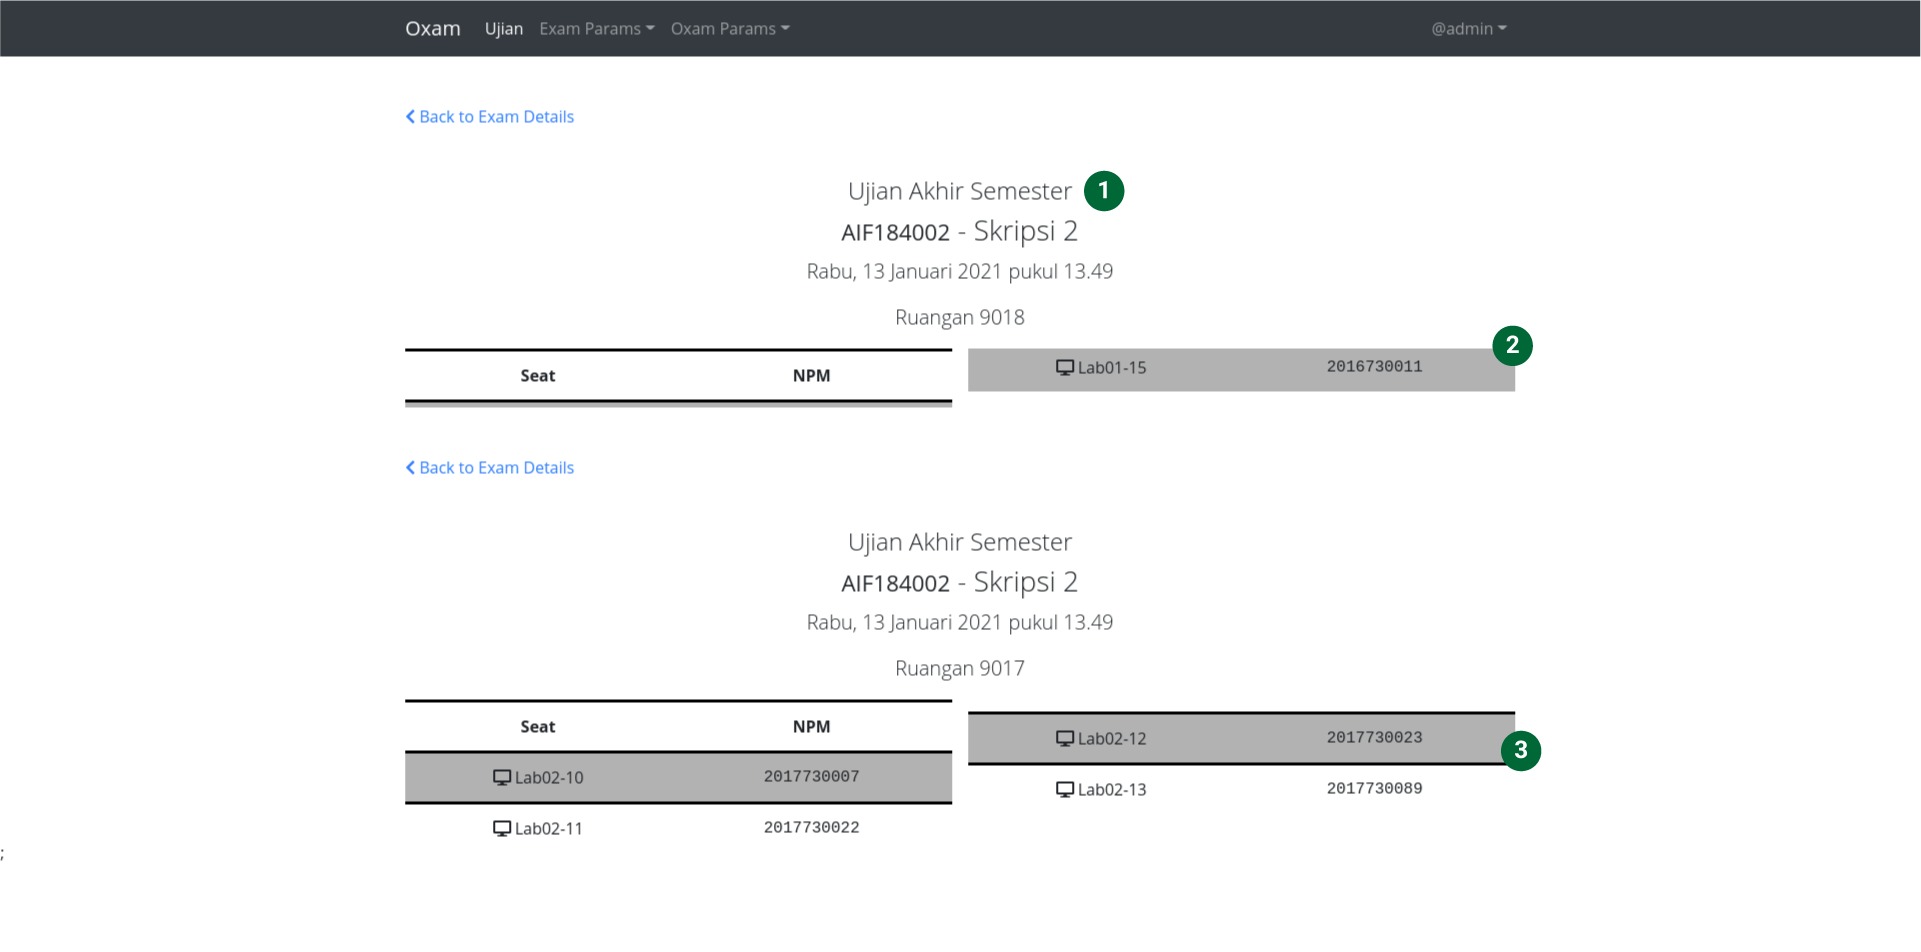
\includegraphics[width=0.7\paperwidth]{Gambar/implemented-interface/admin/absen-pintu.png}
        \caption{Tangkapan layar absensi untuk ditempel pada pintu.}
        \label{fig:screenshot-admin-absen-pintu}
    \end{figure}
    \begin{figure}
        \centering
        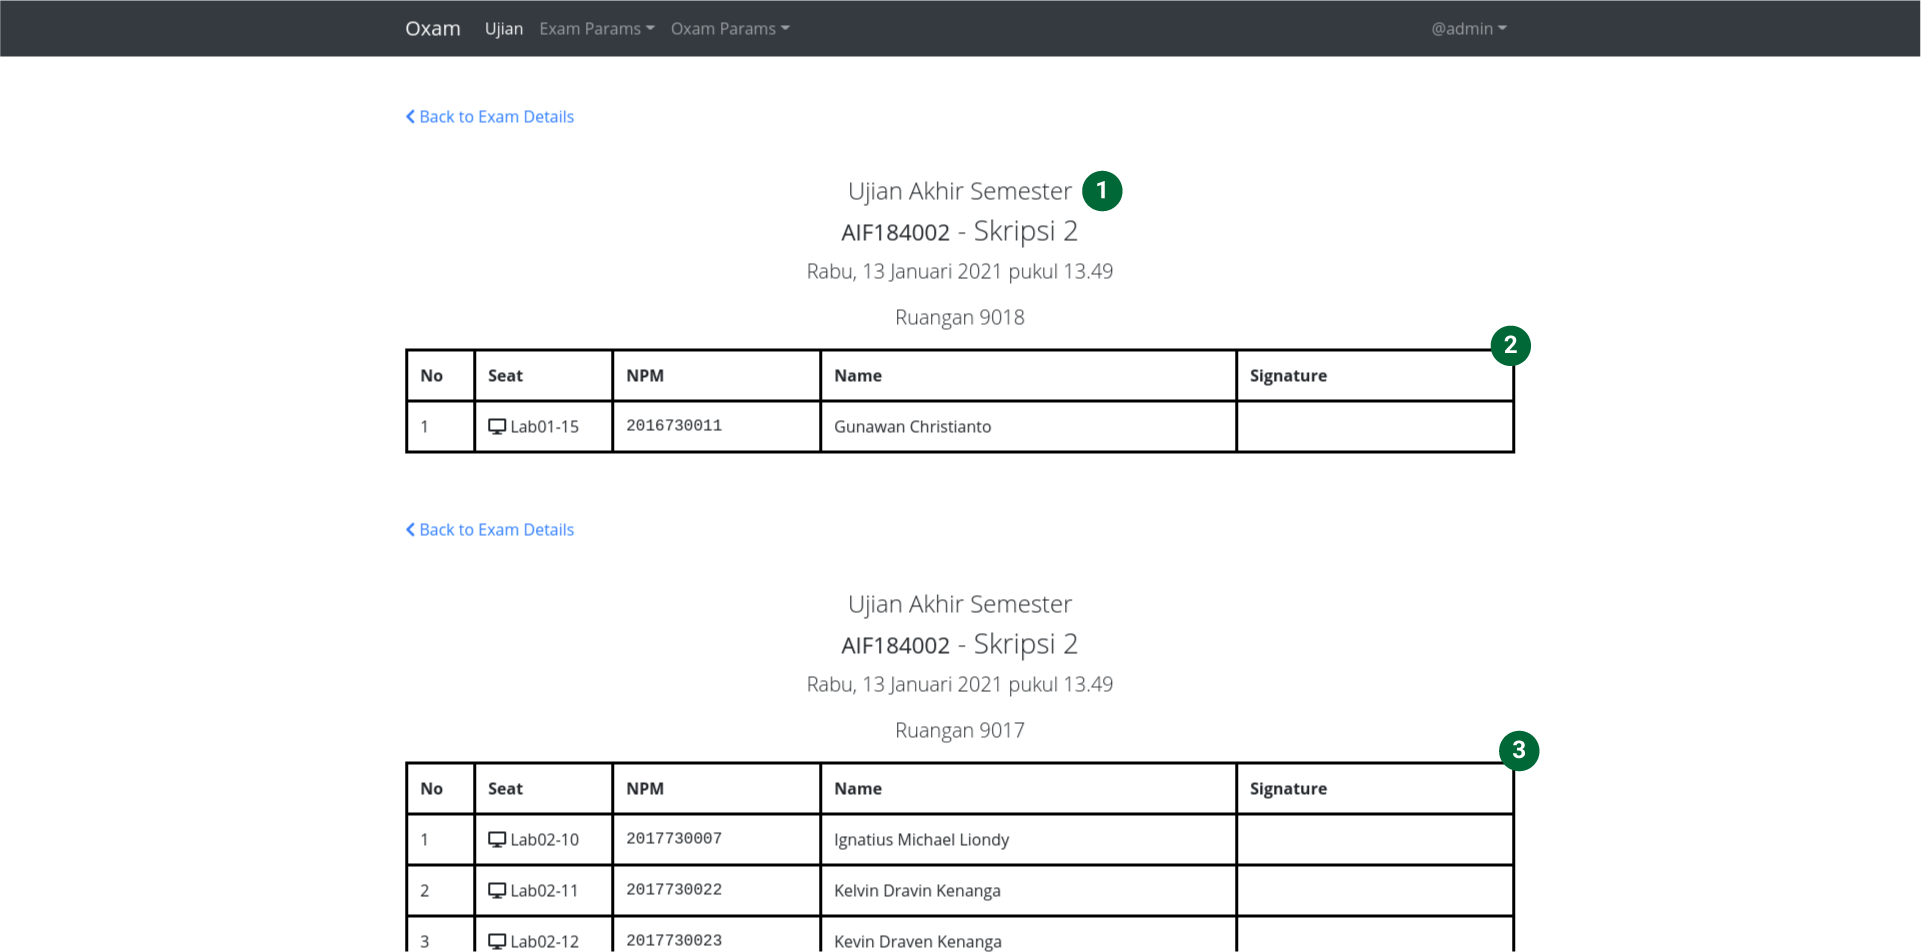
\includegraphics[width=0.7\paperwidth]{Gambar/implemented-interface/admin/absen-ttd.png}
        \caption{Tangkapan layar absensi untuk tanda tangan peserta.}
        \label{fig:screenshot-admin-absen-ttd}
    \end{figure}
    Tampilan absensi untuk peserta dapat dilihat pada Gambar \ref{fig:screenshot-admin-absen-pintu} dan
    \ref{fig:screenshot-admin-absen-ttd}. Pada tangkapan layar untuk absensi yang ditempel ke pintu,
    dapat dilihat pada Gambar \ref{fig:screenshot-admin-absen-pintu}, terdiri dari
    \begin{itemize}
        \item Poin 1: Informasi singkat tentang ujian.
        \item Poin 2: Daftar peserta dengan baris yang dibuat terarsir. 
        \item Poin 3: Daftar peserta untuk ruangan lain.
    \end{itemize}
    Sedangkan pada absen untuk tanda tangan yang dapat dilihat pada Gambar \ref{fig:screenshot-admin-absen-ttd},
    terdiri dari
    \begin{itemize}
        \item Poin 1: Informasi singkat tentang ujian.
        \item Poin 2: Daftar peserta dengan baris yang dibuat terbingkai dan diurutkan berdasarkan nomor komputer. 
        \item Poin 3: Daftar peserta untuk ruangan lain.
    \end{itemize}
    
    \begin{figure}
        \centering
        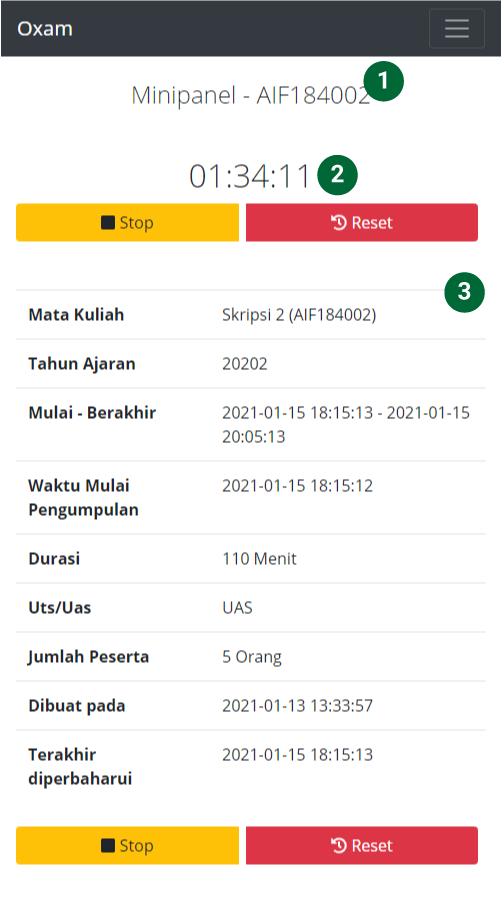
\includegraphics[width=0.3\paperwidth]{Gambar/implemented-interface/admin/ujian-minipanel.png}
        \caption{Tangkapan layar panel perangkat bergerak.}
        \label{fig:screenshot-admin-exam-minipanel}
    \end{figure}
    Tampilan berikutnya adalah tampilan panel admin mini, dapat dilihat pada Gambar
    \ref{fig:screenshot-admin-exam-minipanel}. Tampilan tersebut memiliki poin yang menunjukkan
    \begin{itemize}
        \item Poin 1: Informasi singkat tentang ujian.
        \item Poin 2: Timer ujian
        \item Poin 3: Tombol kontrol timer ujian
    \end{itemize}
    
    \begin{figure}
        \centering
        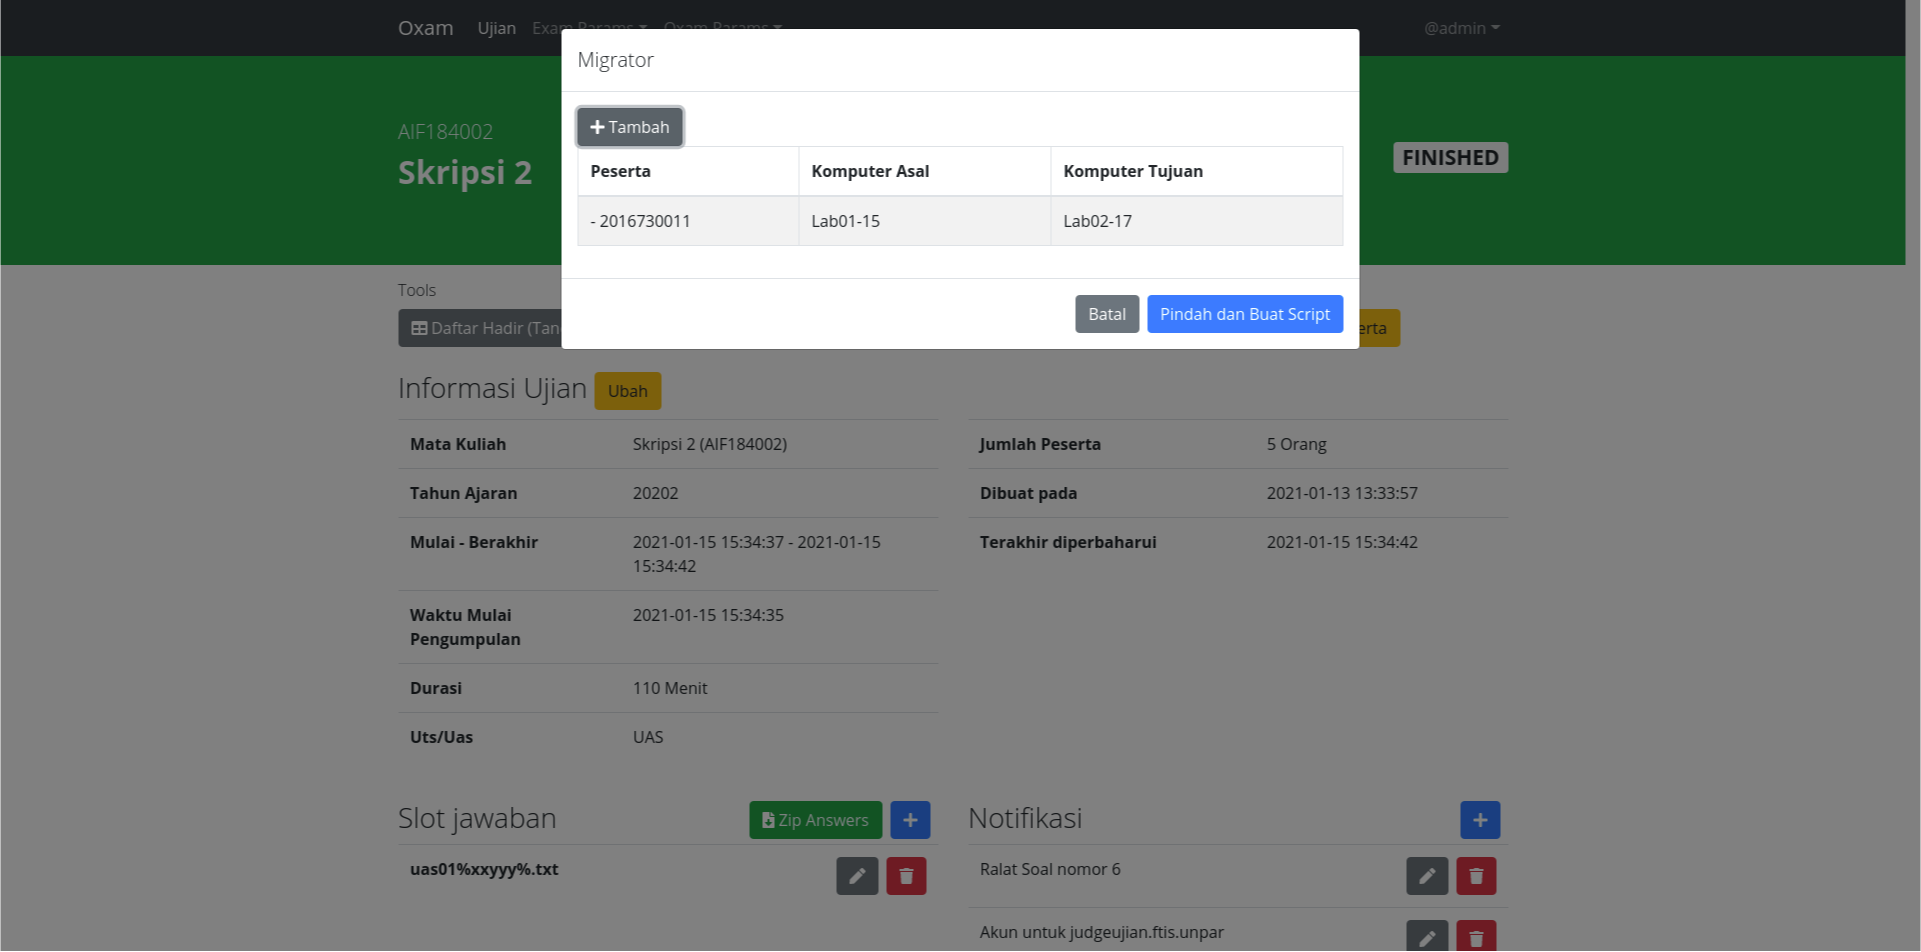
\includegraphics[width=0.7\paperwidth]{Gambar/implemented-interface/admin/migrator-home.png}
        \caption{Tangkapan layar untuk pemindah peserta.}
        \label{fig:screenshot-admin-migrator-home}
    \end{figure}
    \begin{figure}
        \centering
        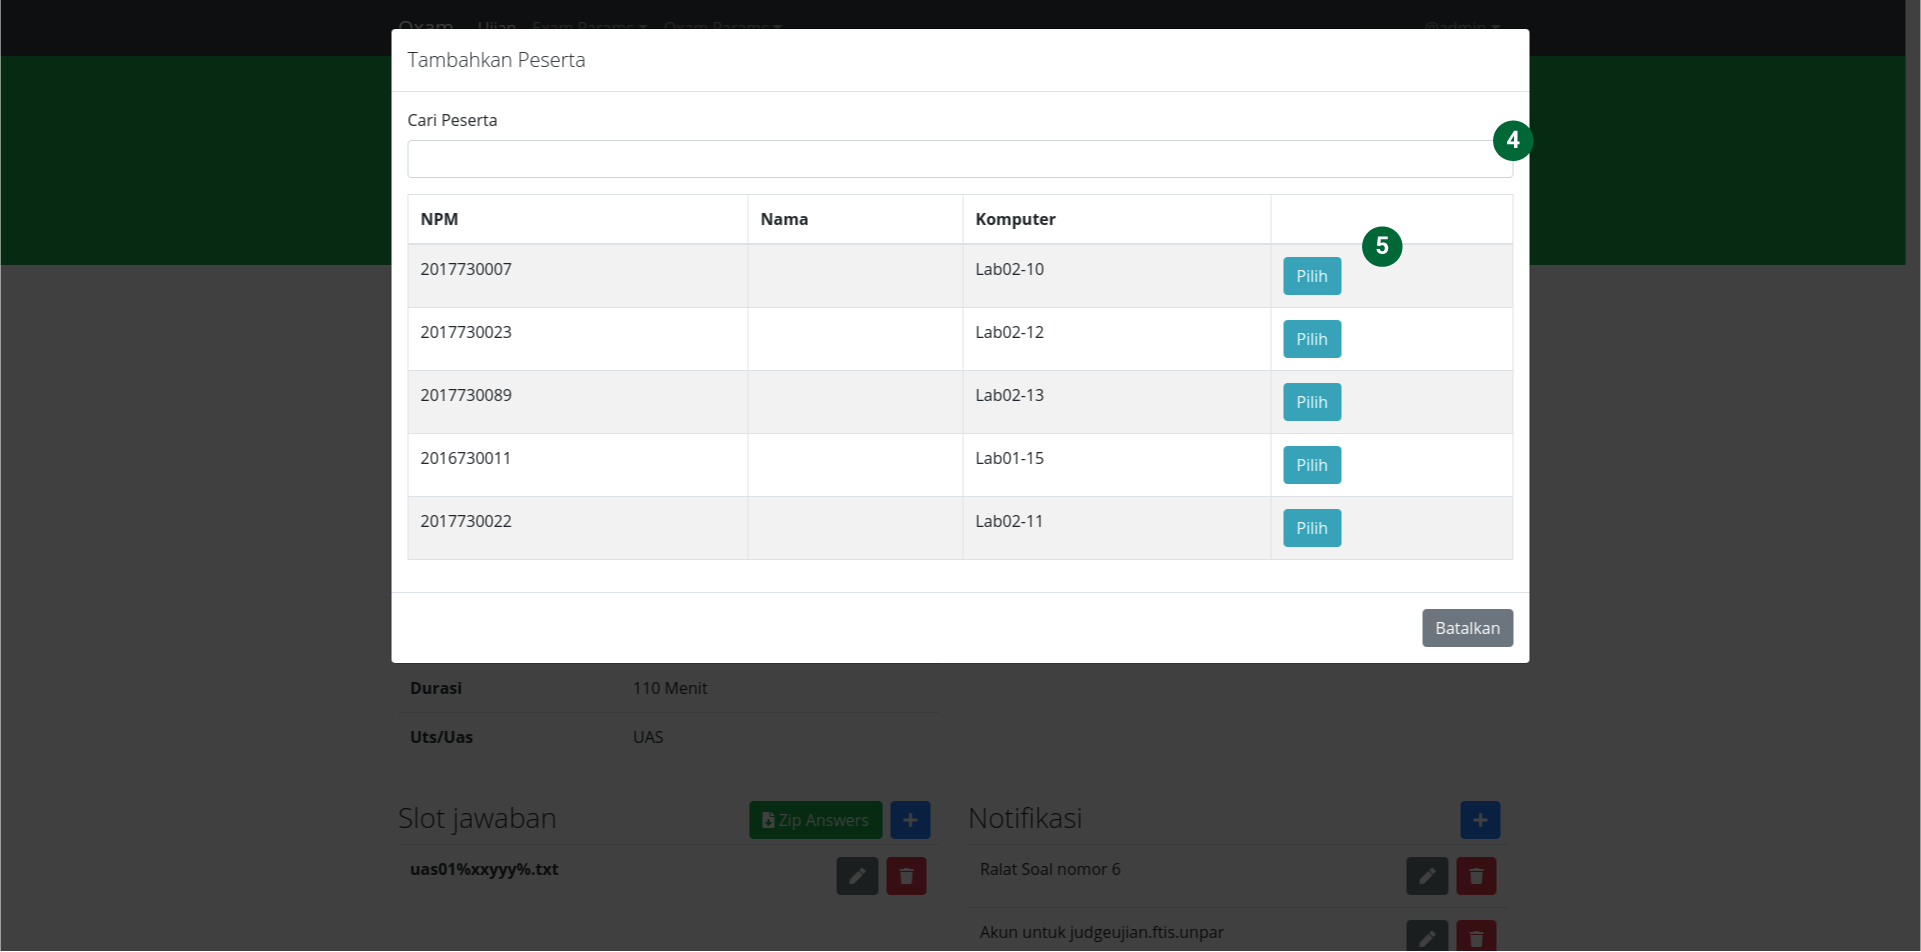
\includegraphics[width=0.7\paperwidth]{Gambar/implemented-interface/admin/migrator-picker-peserta.png}
        \caption{Tangkapan layar untuk pemindah peserta, langkah memilih peserta.}
        \label{fig:screenshot-admin-migrator-picker-peserta}
    \end{figure}
    \begin{figure}
        \centering
        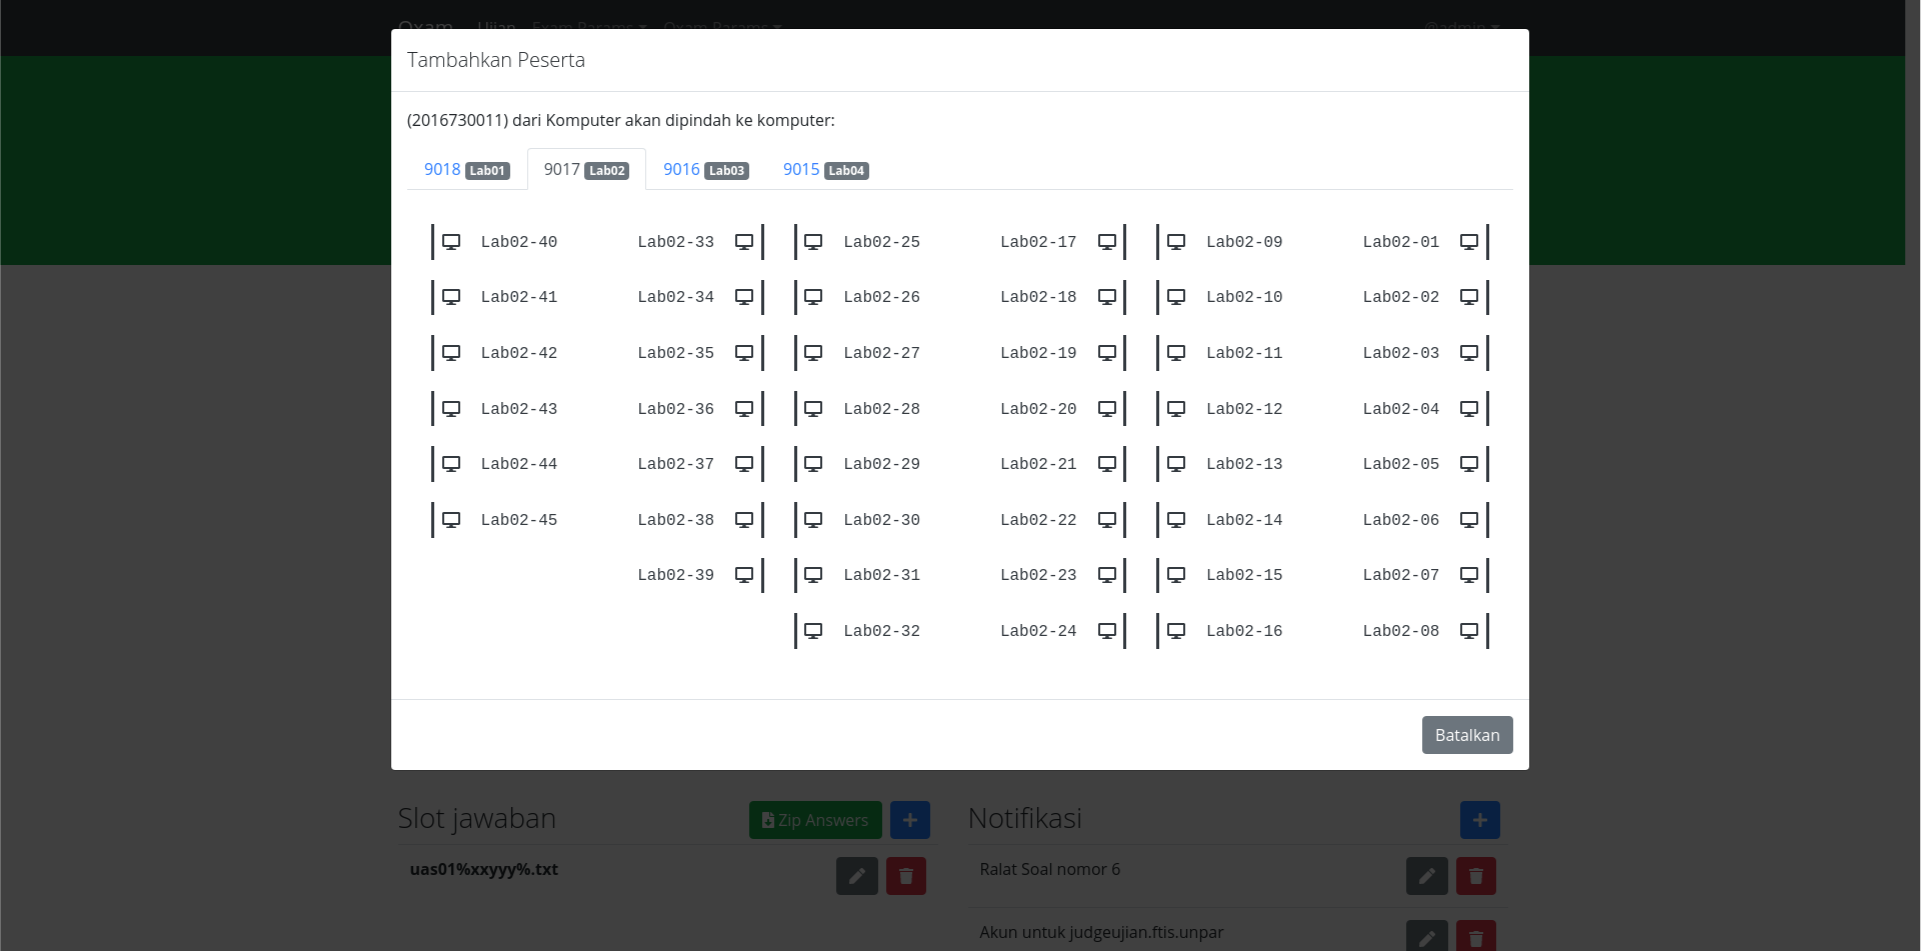
\includegraphics[width=0.7\paperwidth]{Gambar/implemented-interface/admin/migrator-picker-komputer.png}
        \caption{Tangkapan layar untuk pemindah peserta, langkah memilih komputer.}
        \label{fig:screenshot-admin-picker-komputer}
    \end{figure}
    \begin{figure}
        \centering
        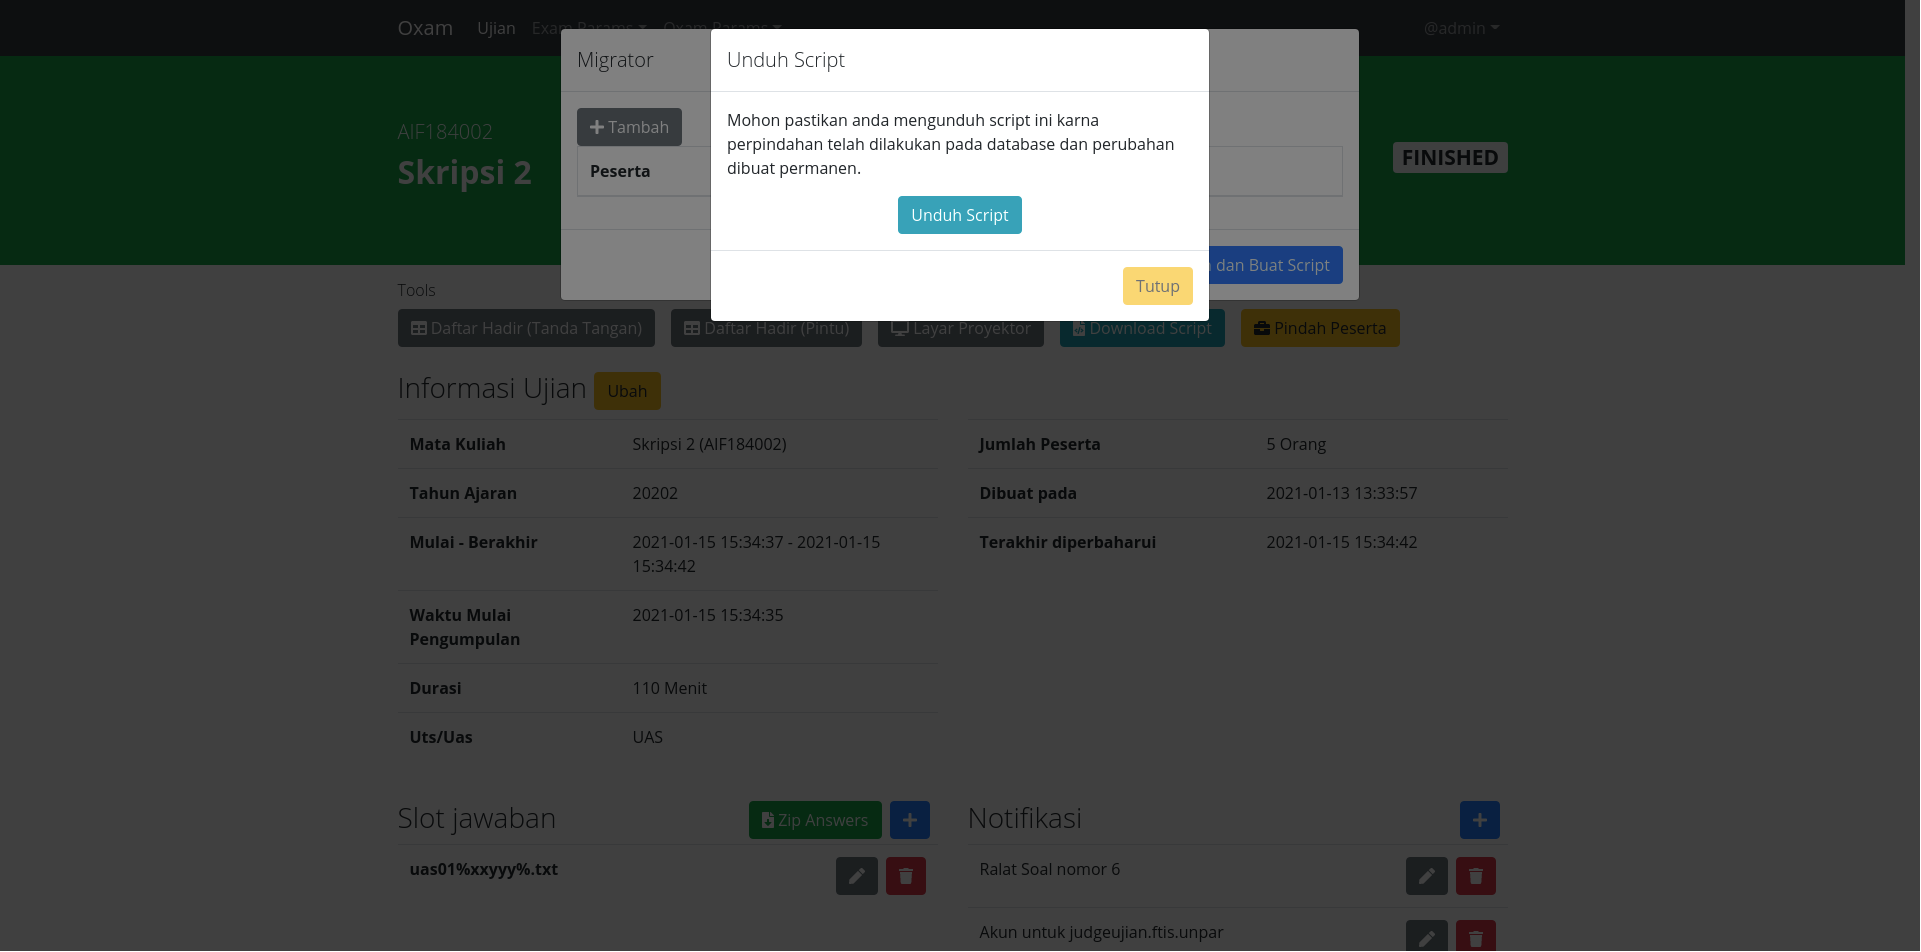
\includegraphics[width=0.7\paperwidth]{Gambar/implemented-interface/admin/migrator-download.png}
        \caption{Tangkapan layar untuk pemindah peserta, langkah mengunduh \textit{script}.}
        \label{fig:screenshot-admin-picker-download}
    \end{figure}
    Fitur untuk memindahkan tempat duduk peserta dapat dilihat pada gambar \ref{fig:screenshot-admin-migrator-home},
    \ref{fig:screenshot-admin-migrator-picker-peserta}, \ref{fig:screenshot-admin-picker-komputer}, dan 
    \ref{fig:screenshot-admin-picker-download}.
    Pada gambar-gambar tersebut terdapat poin-poin yang menunjukkan beberapa bagian tertentu pada tangkapan layar tersebut.
    Poin-poin tersebut terdiri dari
    \begin{itemize}
        \item Poin 1: Tombol tambah untuk mencari peserta yang akan dipindahkan.
        \item Poin 2: Daftar peserta yang akan dipindahkan, dan lokasi baru yang akan peserta dapatkan.
        \item Poin 3: Tombol aksi untuk melakukan pemindahan dan buat sript, serta tombol batal.
        \item Poin 4: Berisi bidang pencarian peserta cepat.
        \item Poin 5: Daftar peserta yang ada pada ujian ini.
        \item Poin 6: NPM peserta yang akan dipindah.
        \item Poin 7: Peta tempat duduk ruangan untuk memilih komputer baru.
        \item Poin 8: Pengunduhan \textit{script}.
    \end{itemize}
    
    \begin{figure}
        \centering
        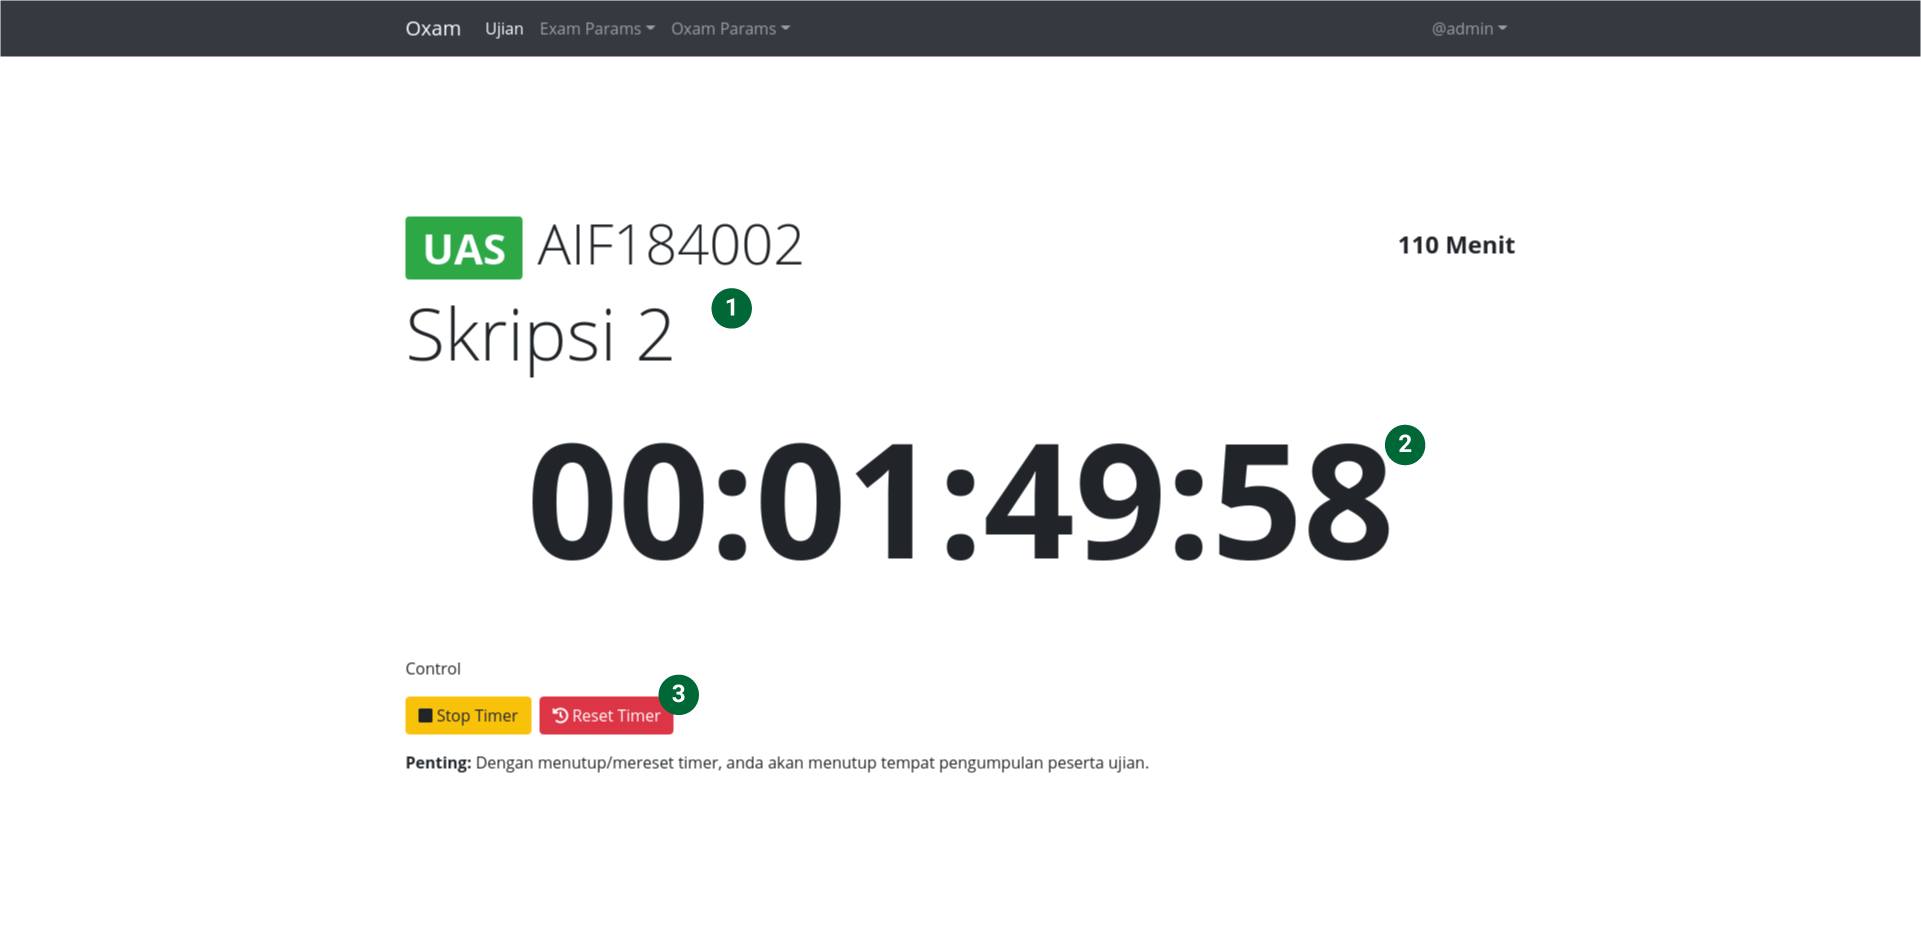
\includegraphics[width=0.7\paperwidth]{Gambar/implemented-interface/admin/timer-admin.png}
        \caption{Tangkapan layar untuk layar proyektor Admin.}
        \label{fig:screenshot-admin-exam-projector}
    \end{figure}
    Tampilan layar proyektor untuk peran admin dapat dilihat pada Gambar \ref{fig:screenshot-admin-exam-projector}.
    Pada bagian tersebut terlihat beberapa poin yang terdiri dari
    \begin{itemize}
        \item Poin 1: Informasi singkat ujian dan total durasi.
        \item Poin 2: Timer sisa waktu ujian.
        \item Poin 3: Tombol kontrol timer.
    \end{itemize}
    
    \begin{figure}
        \centering
        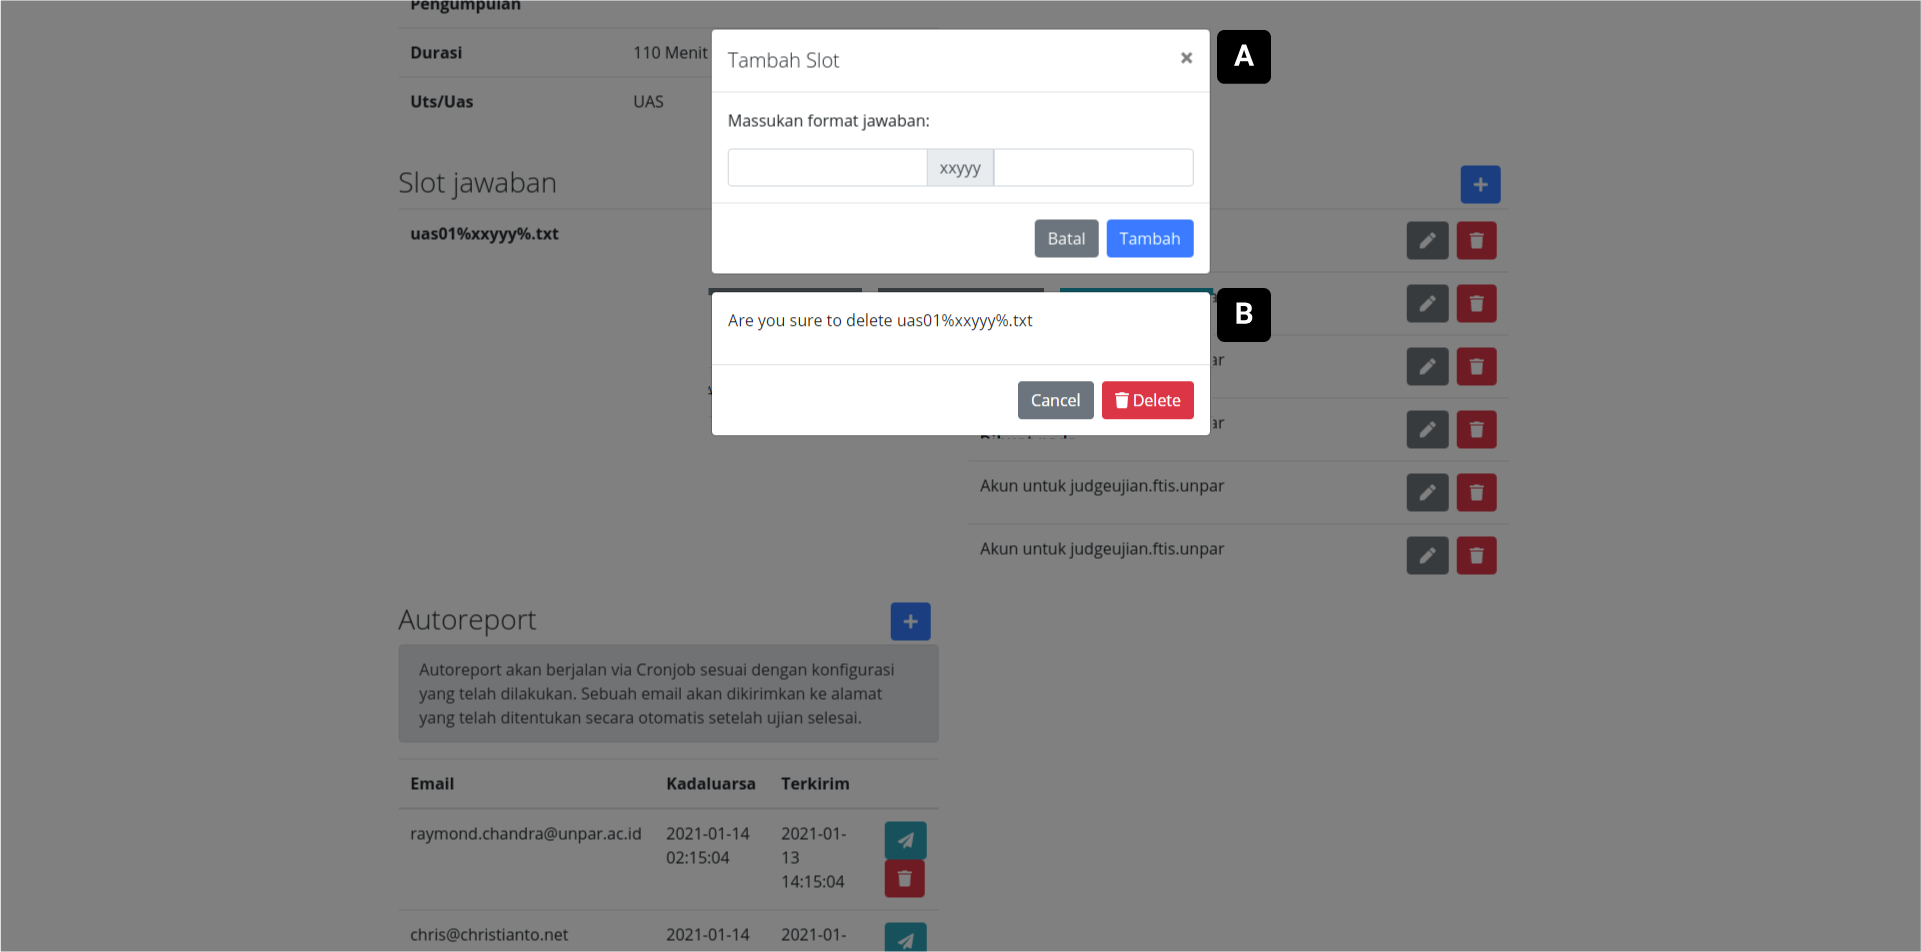
\includegraphics[width=0.7\paperwidth]{Gambar/implemented-interface/admin/ujian-slot-tambah.png}
        \caption{Tangkapan layar untuk slot jawaban. \\ (A) untuk menambahkan slot jawaban, (B) untuk menghapus slot jawaban.}
        \label{fig:screenshot-admin-slot-jawab}
    \end{figure}
    Tangkapan layar berikutnya adalah fitur untuk slot jawaban. Pada Gambar \ref{fig:screenshot-admin-slot-jawab}
    bagian A, modal akan menanyakan format jawaban yang ingin ditambahkan dan tombol aksinya. Sedangkan bagian
    B menunjukkan modal konfirmasi penghapusan slot jawaban tersebut serta tombol aksinya.
    
    \begin{figure}
        \centering
        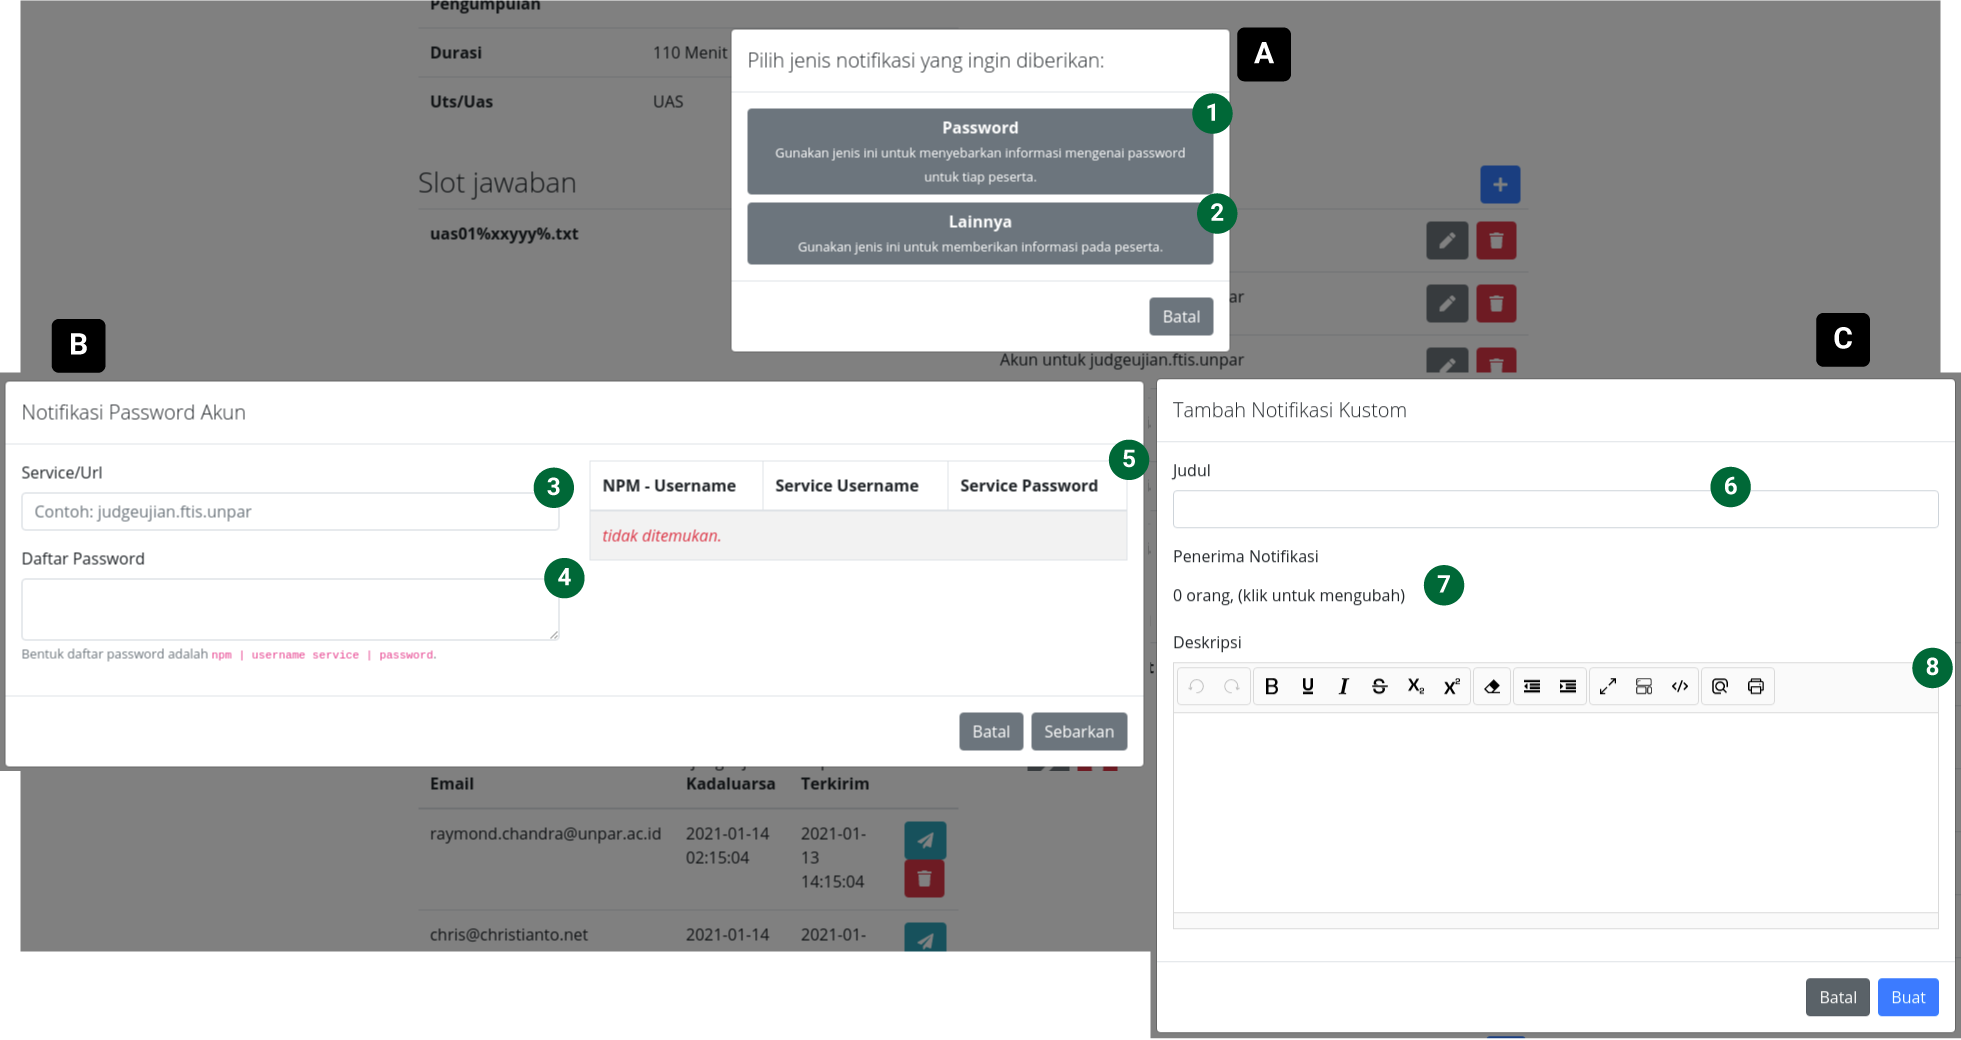
\includegraphics[width=0.7\paperwidth]{Gambar/implemented-interface/admin/ujian-notifikasi.png}
        \caption{Tangkapan layar untuk fitur notifikasi. \\ (A) modal pemilihan jenis. (B) modal notifikasi kata sandi. (C) modal untuk notifikasi lainnya.}
        \label{fig:screenshot-admin-notif}
    \end{figure}
    \begin{figure}
        \centering
        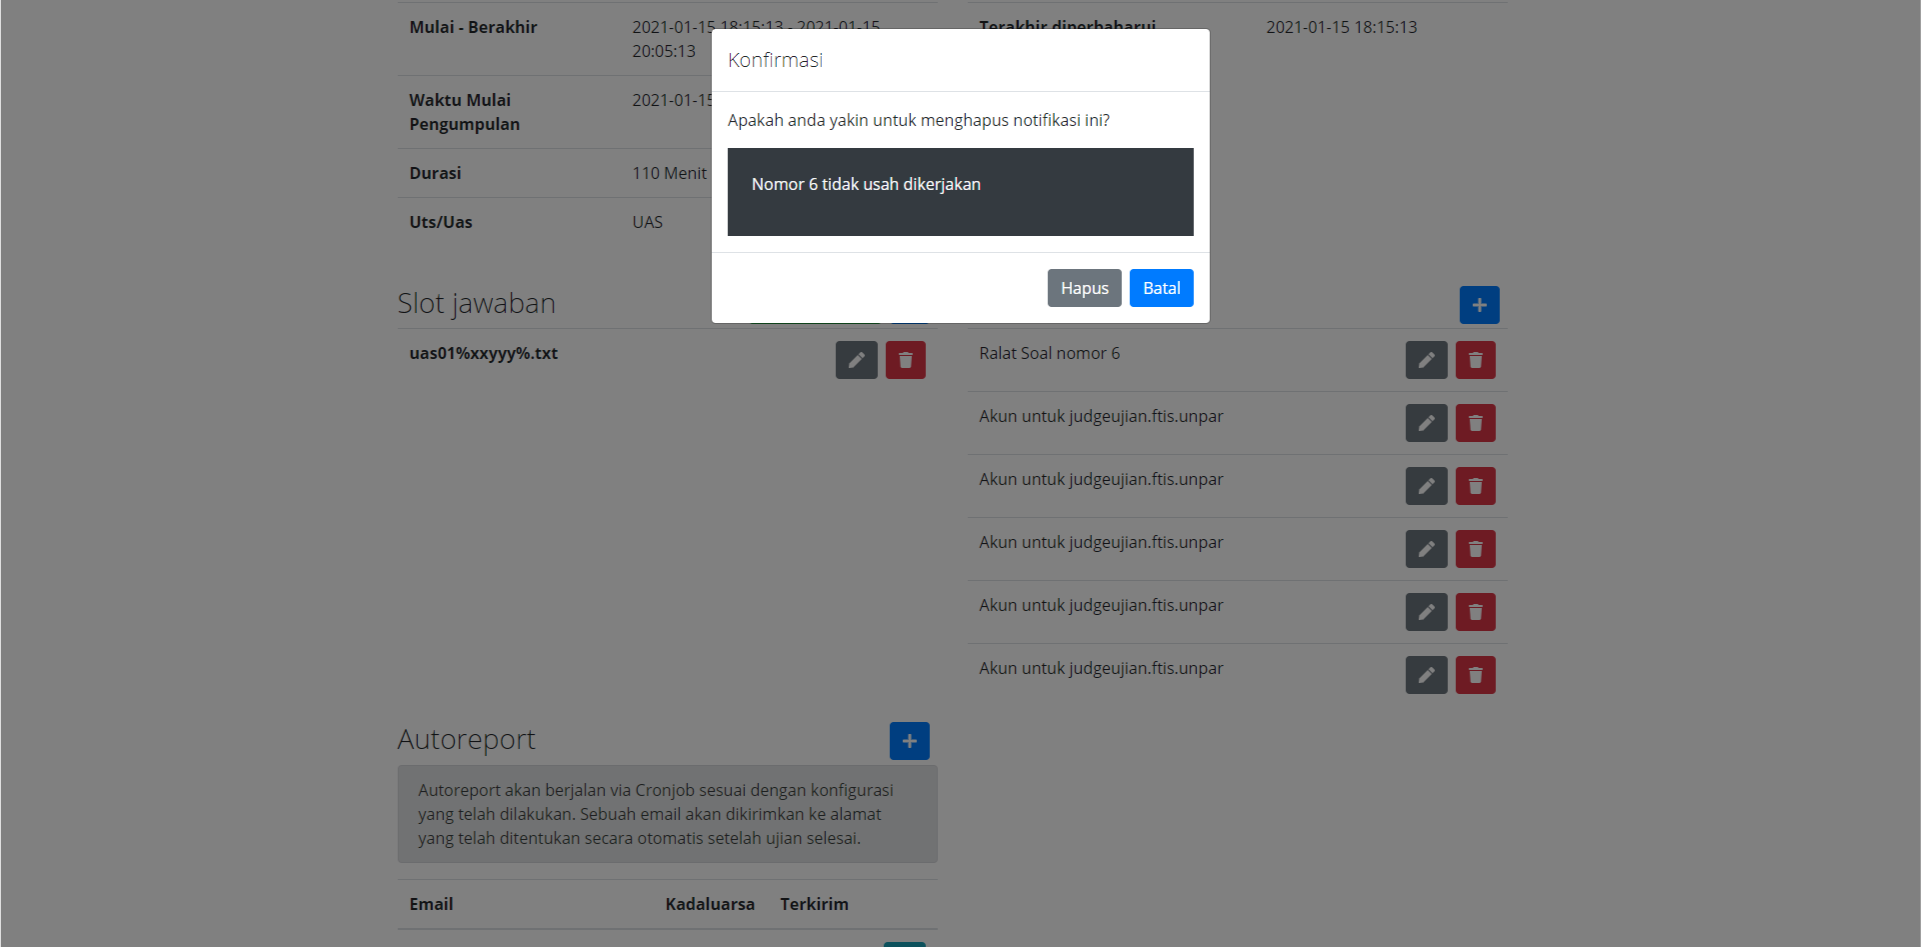
\includegraphics[width=0.7\paperwidth]{Gambar/implemented-interface/admin/ujian-notifikasi-delete.png}
        \caption{Tangkapan layar untuk konfirmasi penghapusan notifikasi.}
        \label{fig:screenshot-admin-notif-delete}
    \end{figure}
    Hasil implementasi untuk fitur notifikasi dapat dilihat pada Gambar \ref{fig:screenshot-admin-notif} dan
    \ref{fig:screenshot-admin-notif-delete}. Tangkapan layar dengan bagian A, B dan C pada Gambar 
    \ref{fig:screenshot-admin-notif} memiliki poin-poin yang terdiri dari
    \begin{itemize}
        \item Poin 1: Tombol jenis notifikasi kata sandi.
        \item Poin 2: Tombol jenis notifikasi lainnya.
        \item Poin 3: Bidang nama layanan untuk kredensial yang akan dibagikan.
        \item Poin 4: Bidang daftar kredensial tersebut.
        \item Poin 5: Pratinjau dari daftar kredensial yang akan dibagian.
        \item Poin 6: Bidang judul notifikasi jenis lainnya.
        \item Poin 7: Daftar penerima notifikasi.
        \item Poin 8: Badan notifikasi untuk jenis lainnya.
    \end{itemize}
    Sedangkan pada Gambar \ref{fig:screenshot-admin-notif-delete}, modal konfirmasi penghapusan akan menampilkan
    informasi badan notifikasi dan tombol aksi penghapusan atau pembatalan.
    
    \subsubsection{Pengelolaan Entitas}
    \begin{figure}
        \centering
        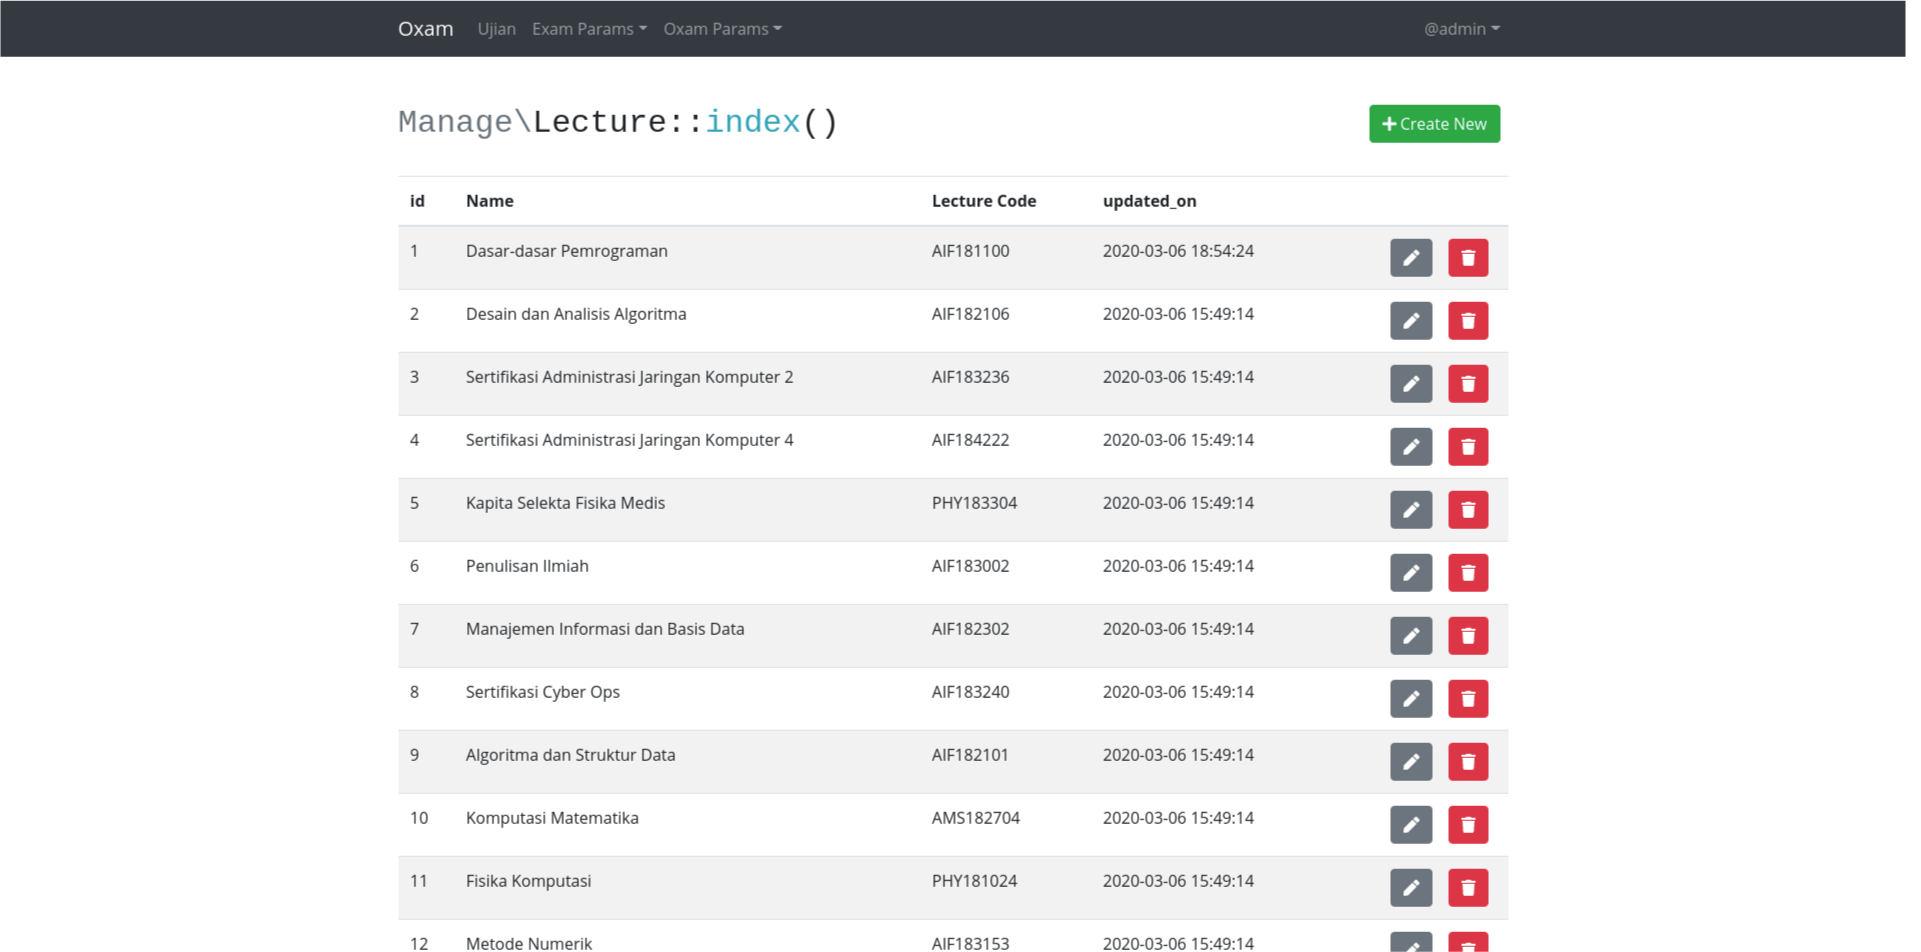
\includegraphics[width=0.7\paperwidth]{Gambar/implemented-interface/admin/entity-lister.png}
        \caption{Tangkapan layar untuk daftar entri pada entitas.}
        \label{fig:screenshot-admin-entity-list}
    \end{figure}
    \begin{figure}
        \centering
        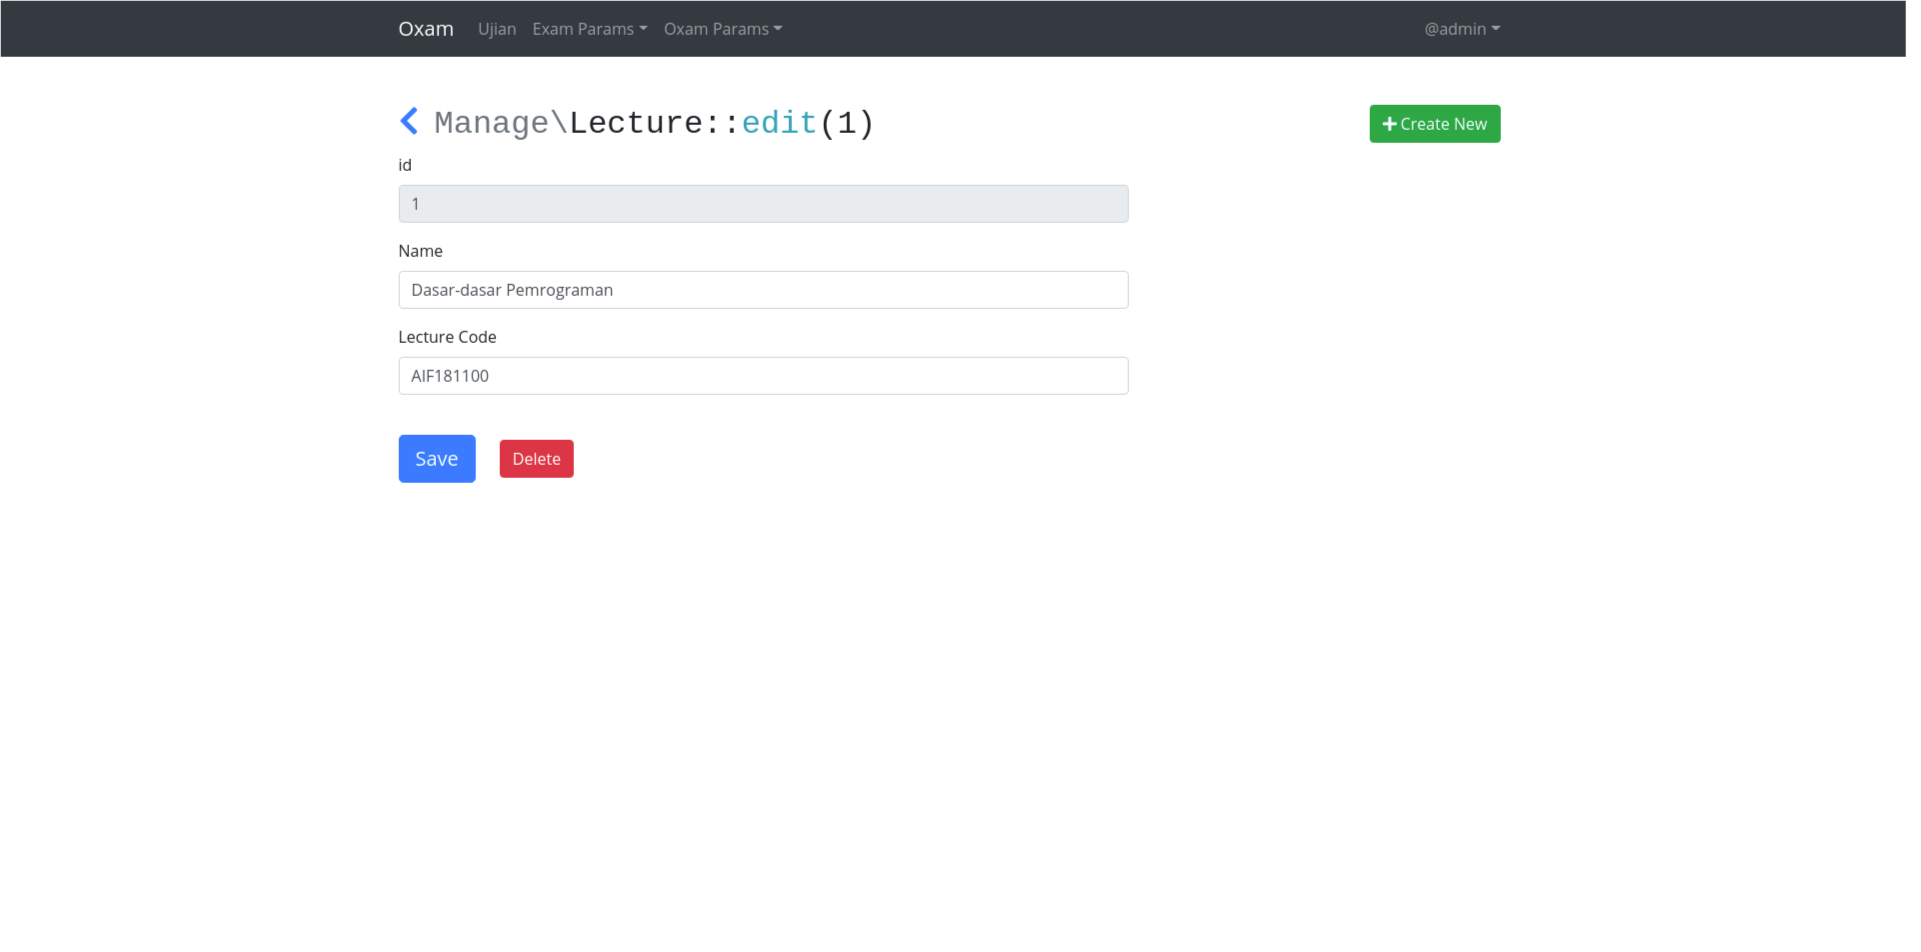
\includegraphics[width=0.7\paperwidth]{Gambar/implemented-interface/admin/entity-editor.png}
        \caption{Tangkapan layar untuk \textit{editor} entri}
        \label{fig:screenshot-admin-entity-edit}
    \end{figure}
    \begin{figure}
        \centering
        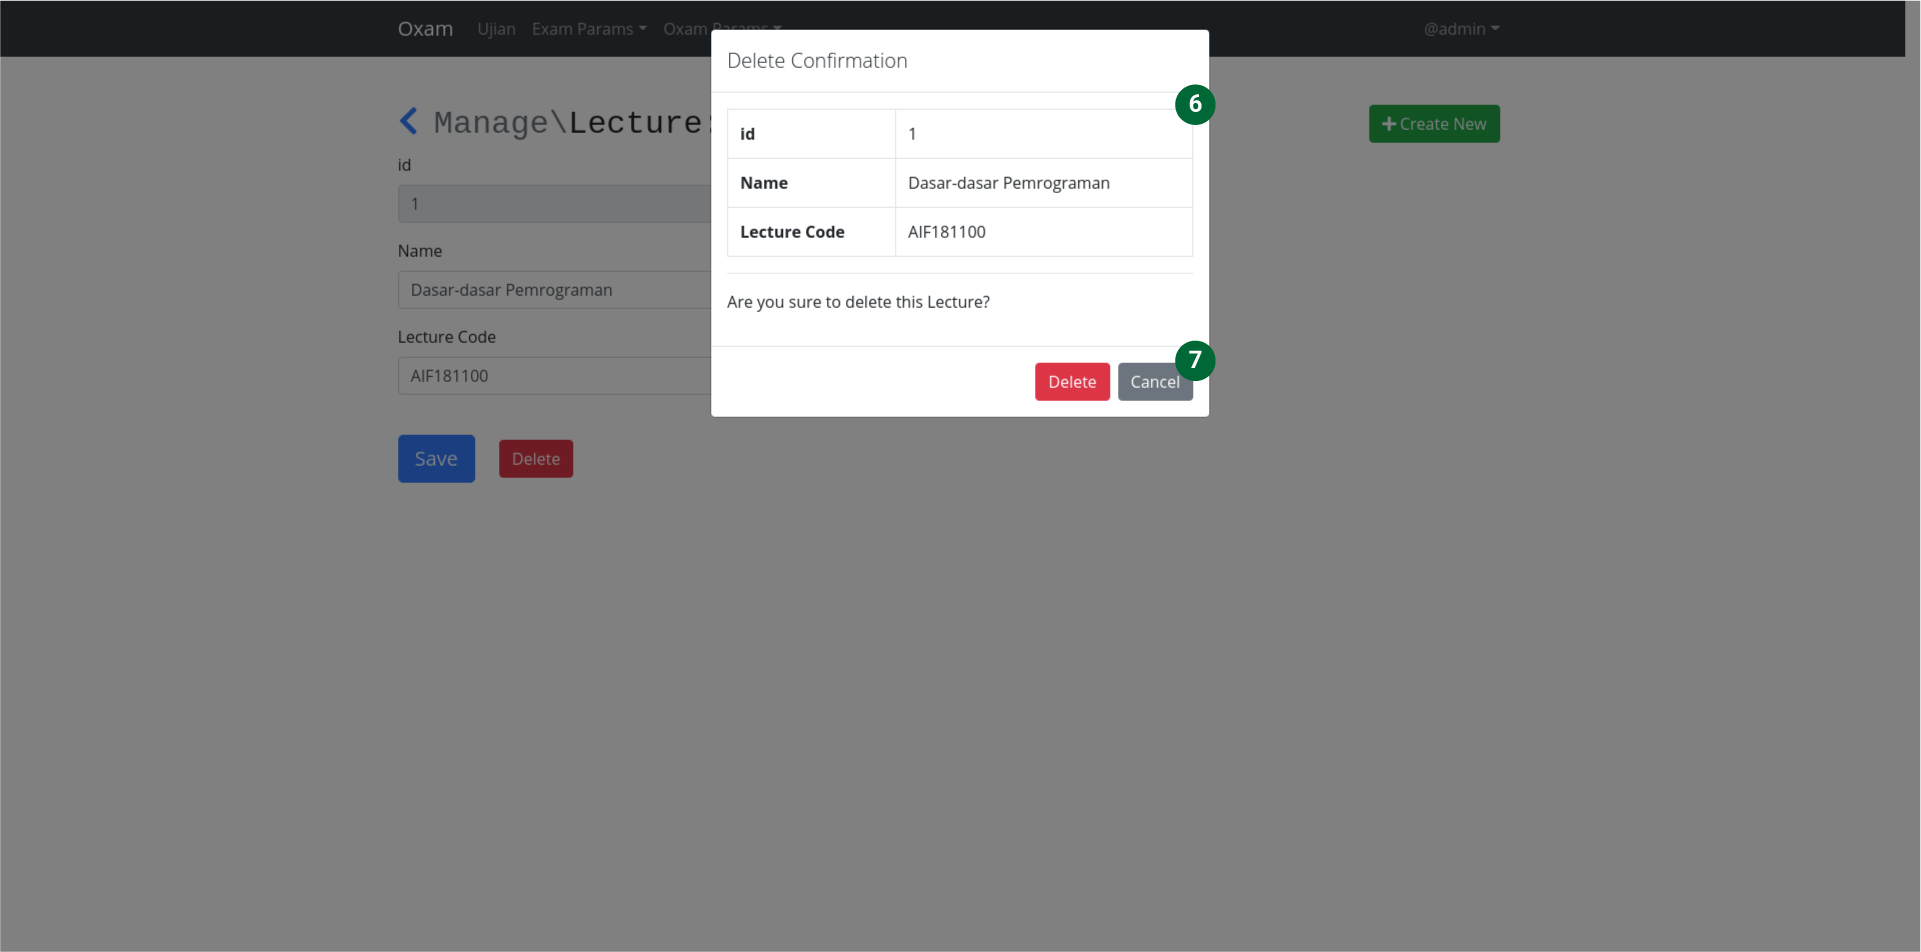
\includegraphics[width=0.7\paperwidth]{Gambar/implemented-interface/admin/entity-delete.png}
        \caption{Tangkapan layar untuk konfirmasi penghapusan entri.}
        \label{fig:screenshot-admin-entity-delete}
    \end{figure}
    Hasil implementasi untuk fitur pengelolaan entitas dapat dilihat pada Gambar \ref{fig:screenshot-admin-entity-list},
    \ref{fig:screenshot-admin-entity-edit}, dan \ref{fig:screenshot-admin-entity-delete}.
    Pada gambar-gambar tersebut terdapat beberapa poin yang terdiri dari
    \begin{itemize}
        \item Poin 1: Tombol membuat entri baru
        \item Poin 2: Daftar entri yang terdapat pada entitas ini, dengan tombol ubah dan hapus.
        \item Poin 3: Informasi ID entri yang akan diubah.
        \item Poin 4: Formulir data yang terdapat pada entri.
        \item Poin 5: Tombol aksi simpan dan hapus.
        \item Poin 6: Tabel data yang terdapat pada entri.
        \item Poin 7: Tombol aksi untuk menghapus dan batalkan penghapusan.
    \end{itemize}
    
    
    \subsection{Halaman untuk Dosen Pengawas / Layar Proyektor}
    \begin{figure}
        \centering
        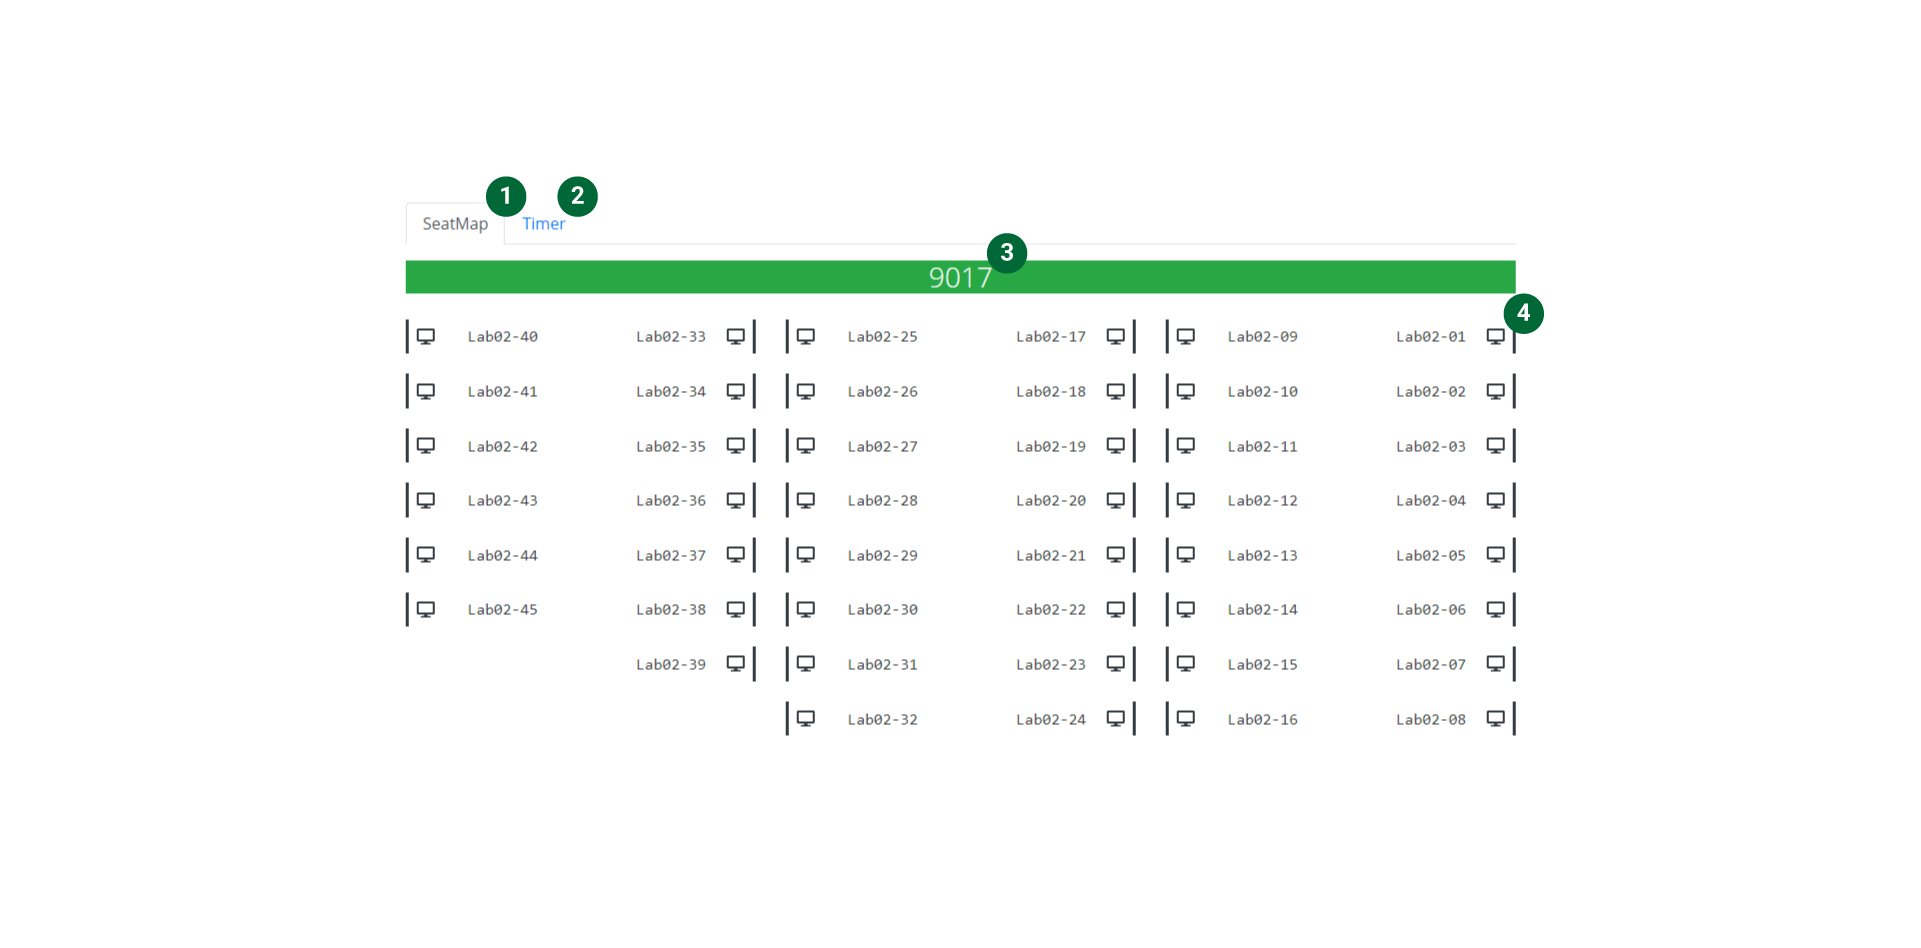
\includegraphics[width=0.7\paperwidth]{Gambar/implemented-interface/pengawas/seatmap.png}
        \caption{Tangkapan layar untuk tampilan denah tempat duduk ruangan ujian.}
        \label{fig:screenshot-pengawas-seatmap}
    \end{figure}
    \begin{figure}
        \centering
        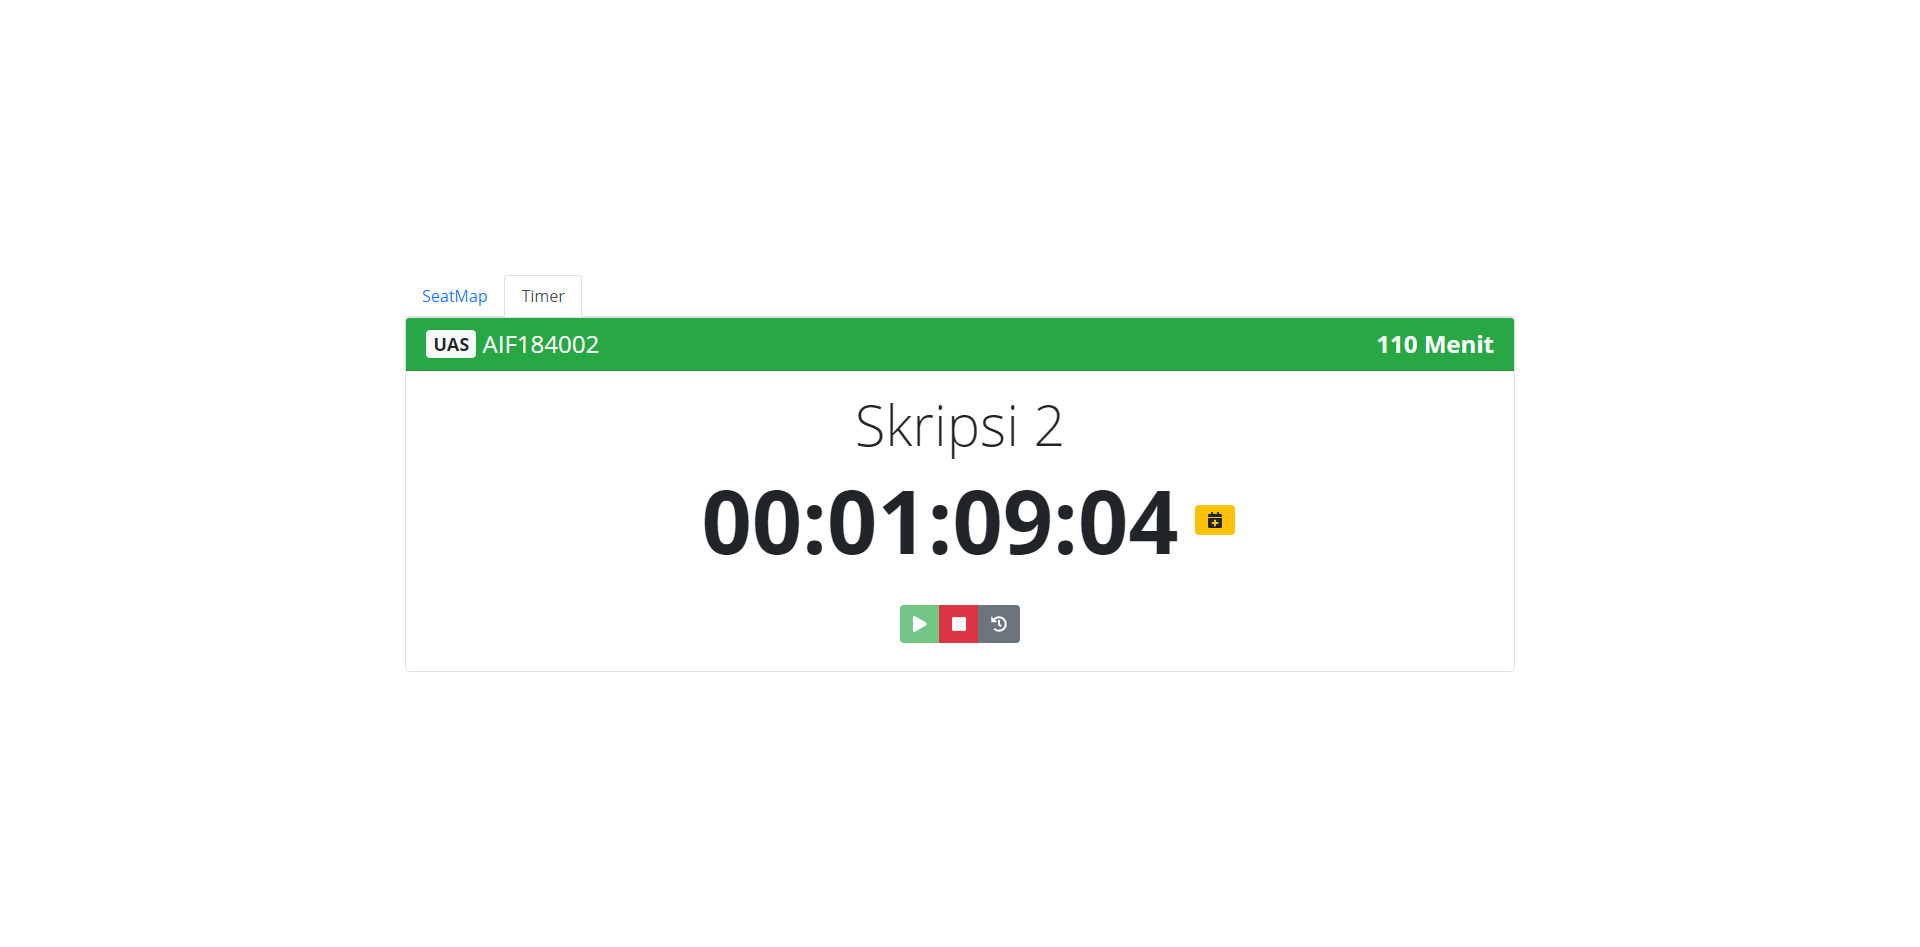
\includegraphics[width=0.7\paperwidth]{Gambar/implemented-interface/pengawas/timer.png}
        \caption{Tangkapan layar untuk tampilan timer untuk ditampilkan pada proyektor.}
        \label{fig:screenshot-pengawas-timer}
    \end{figure}
    \begin{figure}
        \centering
        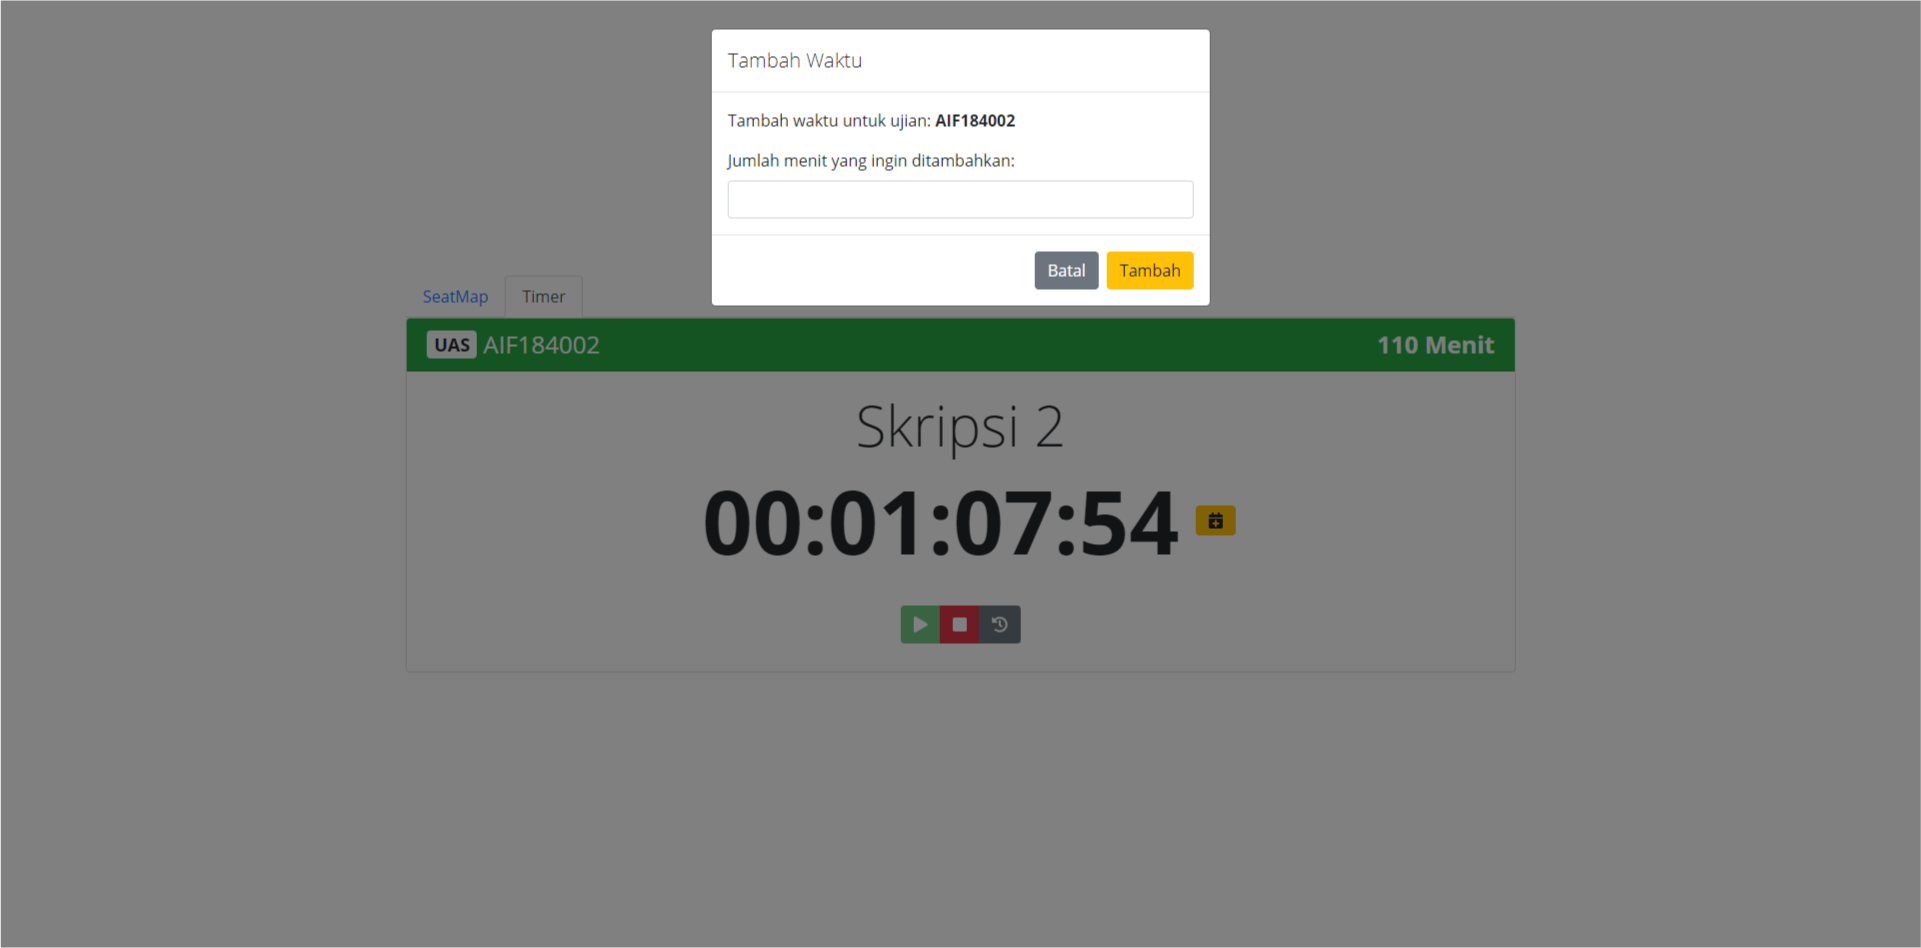
\includegraphics[width=0.7\paperwidth]{Gambar/implemented-interface/pengawas/overtime.png}
        \caption{Tangkapan layar untuk tampilan untuk modal penambahan waktu lebih.}
        \label{fig:screenshot-pengawas-overtime}
    \end{figure}
    Fitur yang digunakan untuk dosen pengawas dapat dilihat hasil implementasinya pada
    Gambar \ref{fig:screenshot-pengawas-seatmap}, \ref{fig:screenshot-pengawas-timer}, dan
    \ref{fig:screenshot-pengawas-overtime}. Gambar tersebut terdiri dari poin-poin sebagai berikut
    \begin{itemize}
        \item Poin 1: Tombol navigasi untuk peta tempat duduk.
        \item Poin 2: Tombol navigasi untuk timer ujian.
        \item Poin 3: Informasi singkat ujian.
        \item Poin 4: Informasi durasi ujian.
        \item Poin 5: Nama mata kuliah ujian
        \item Poin 6: Tombol kontrol timer.
        \item Poin 7: Tombol penambahan waktu lebih untuk ujian.
        \item Poin 8: Nama ruangan yang terbuhung dengan komputer ini.
        \item Poin 9: Denah tempat duduk ruangan.
        \item Poin 10: Informasi ujian singkat untuk konfirmasi.
        \item Poin 11: Bidang banyak menit yang diberikan.
        \item Poin 12: Tombol aksi tambah dan pembatalan.
    \end{itemize}
    
    
    \subsection{Halaman Tambahan untuk Dosen Koordinator}
    \begin{figure}
        \centering
        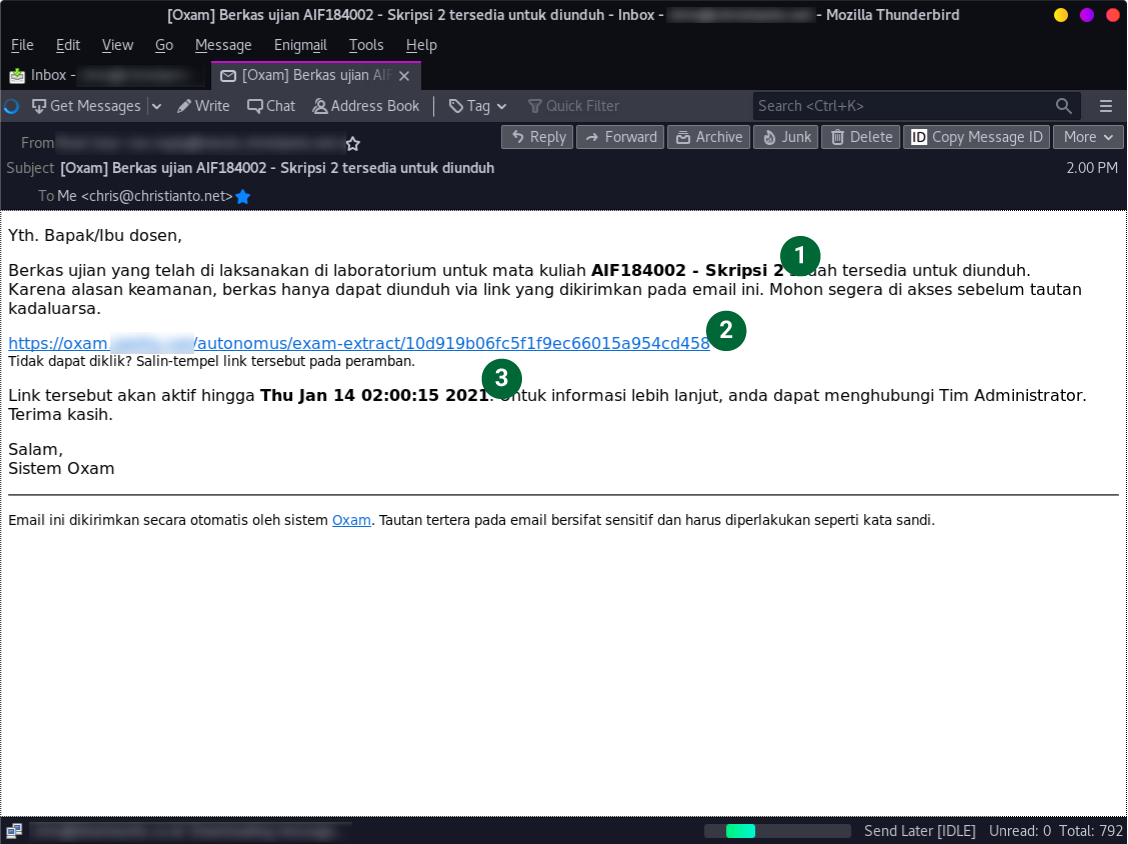
\includegraphics[width=0.7\paperwidth]{Gambar/implemented-interface/extra/extractor-email.png}
        \caption{Tangkapan layar untuk tampilan email yang akan diterima oleh dosen.}
        \label{fig:screenshot-extra-email}
    \end{figure}
    \begin{figure}
        \centering
        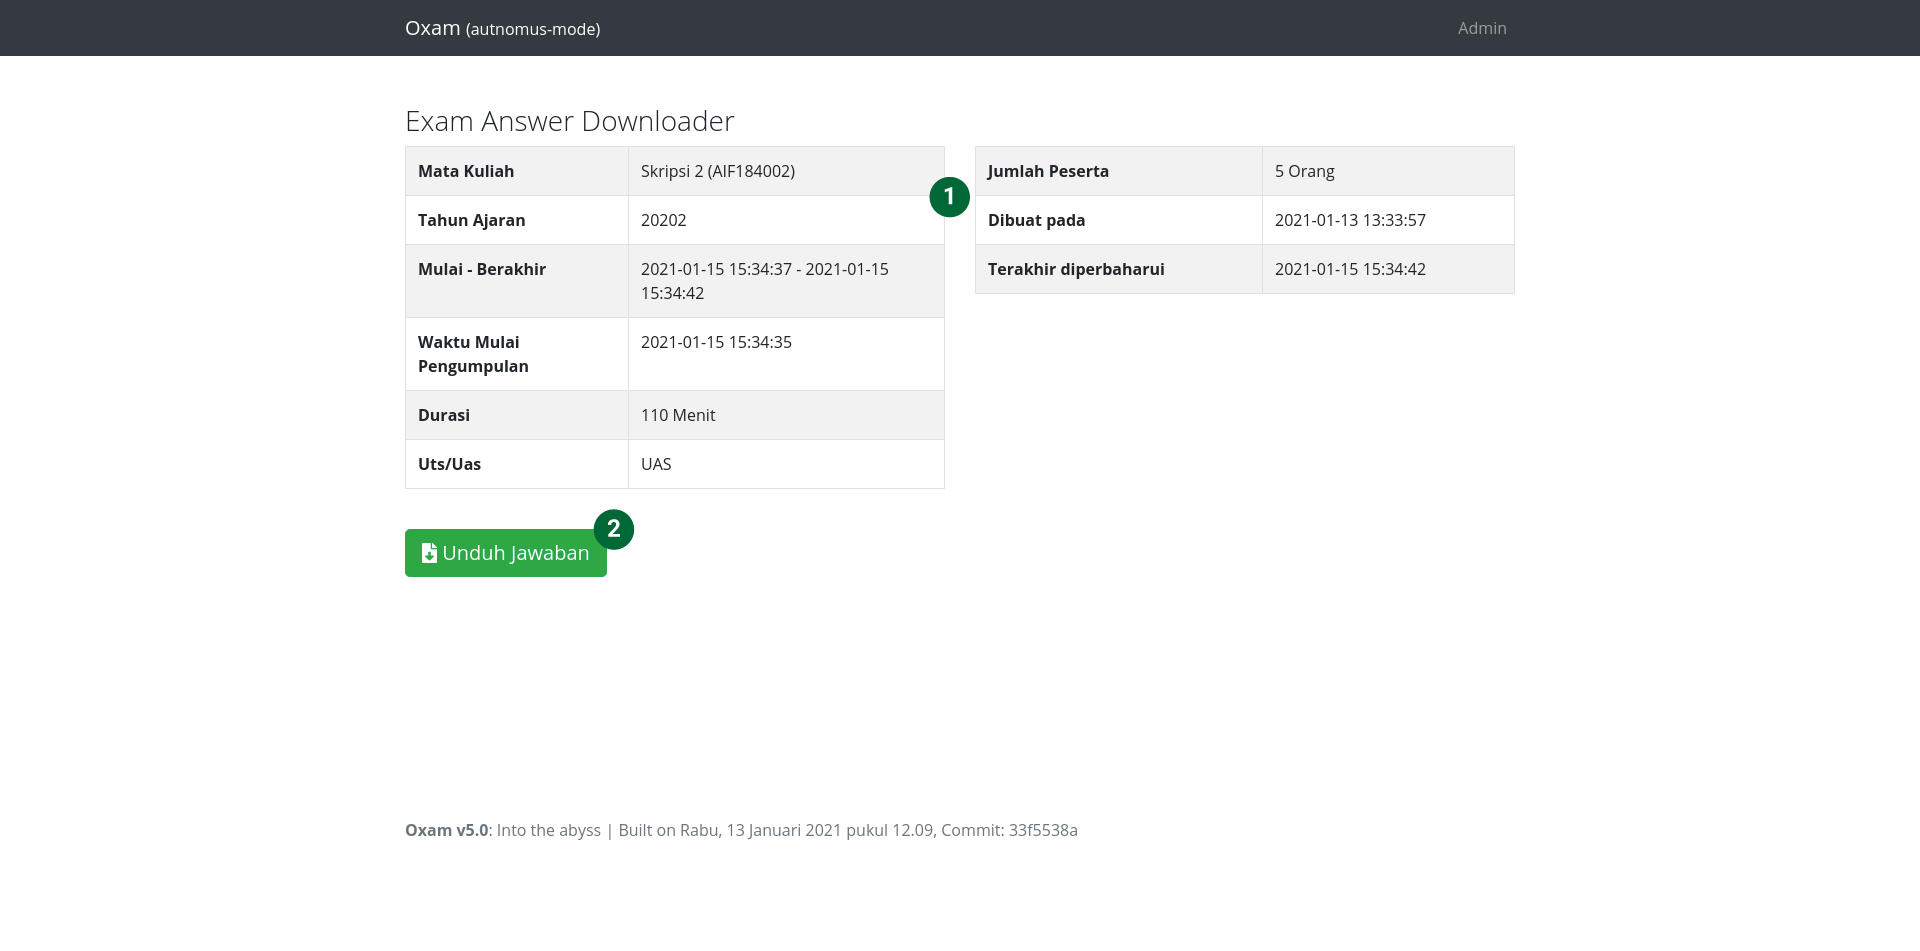
\includegraphics[width=0.7\paperwidth]{Gambar/implemented-interface/extra/extractor-page.png}
        \caption{Tangkapan layar untuk tampilan halaman pengunduhan}
        \label{fig:screenshot-extra-page}
    \end{figure}
    Fitur yang diimplementasi lainnya adalah fitur untuk dosen koordinator mengunduh jawaban peserta ujian.
    Tampilan tersebut dapat dilihat pada Gambar \ref{fig:screenshot-extra-email} dan 
    \ref{fig:screenshot-extra-page}. Pada gambar terdapat poin-poin yang terdiri dari
    \begin{itemize}
        \item Poin 1: Informasi mata kuliah yang diuji.
        \item Poin 2: Tautan untuk melakukan pengunduhan.
        \item Poin 3: Informasi tanggal kadaluarsa tautan tersebut.
        \item Poin 4: Informasi detil ujian.
        \item Poin 5: Tombol pengunduhan jawaban.
    \end{itemize}

% bentuk foldernya
    \subsection{Bentuk Struktur Direktori Penyimpanan Ujian}
    \begin{figure}[hb]
        \centering
        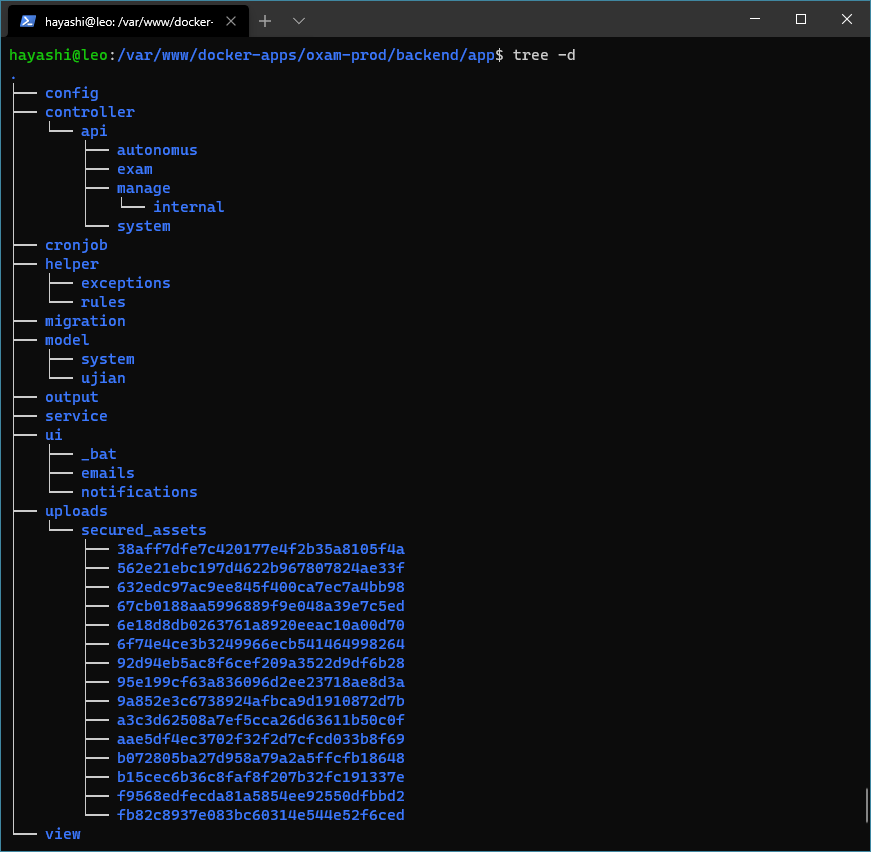
\includegraphics[width=0.6\paperwidth]{Gambar/Screenshot 2021-01-16 014010.png}
        \caption{Tampilan daftar direktori pada sistem backend aplikasi Oxam.}
        \label{fig:dirlisting}
    \end{figure}
    Implementasi untuk pengamanan berkas ujian dilakukan dengan mengacak nama \textit{folder}
    dari tempat penyimpanan ujian. Pada Gambar \ref{fig:dirlisting}, berkas jawaban ujian disimpan pada
    \textit{folder} \texttt{uploads/secured-assets} dengan nama folder yang diacak.


\section{Pengujian Experimental}
    Pengujian experimental dilakukan dengan mendemokan aplikasi pada tim Admin secara langsung. Pada pengujian
    tersebut, Tim Admin akan membuat sebuah mata kuliah dan ujian, lalu mencoba fitur-fitur yang tersedia
    pada sistem Oxam yang baru. Keberhasilan tersebut dilakukan dengan memberikan kuisioner yang kemudian
    Tim Admin isi.
    
    Kuisioner yang akan diberikan pada Tim admin terdiri dari pertanyaan-pertanyaan berikut:
    \begin{enumerate}
        \item Membuat dan mengelola data untuk ujian (mata kuliah, memasukkan peserta, dst) menjadi lebih mudah. \\
            Pertanyaan dibuat dalam bentuk skala 1-4, dengan 1 sangat tidak setuju dan 5 sangat setuju.
            Pertanyaan ditujukan untuk mengethaui apakah pengaturkan dan pengelolaan data untuk ujian dapat
            diatur dengan mudah.

        \item Mengambil dan mengirimkan jawaban menjadi lebih mudah. \\
            Pertanyaan dibuat dalam bentuk skala 1-4, dengan 1 sangat tidak setuju dan 5 sangat setuju.
            Pertanyaan ditujukan untuk mengetahui proses pengambilan dan pengiriman jawaban menjadi lebih
            baik.
        
        \item Membuat ujian menjadi lebih mudah. \\
            Pertanyaan dibuat dalam bentuk skala 1-4, dengan 1 sangat tidak setuju dan 5 sangat setuju.
            Pertanyaan ditujukan untuk mengetahui apakah pembuatan ujian menjadi lebih baik.
        
        \item Upload Jawaban untuk peserta lebih mudah. \\
            Pertanyaan dibuat dalam bentuk skala 1-4, dengan 1 sangat tidak setuju dan 5 sangat setuju.
            Pertanyaan ditujukan untuk mengetahui apakah formulir pengunggahan jawaban untuk peserta
            menjadi lebih baik.
            
        \item Informasi (\textit{password} dan ralat soal) untuk peserta menjadi lebih mudah. \\
            Pertanyaan dibuat dalam bentuk skala 1-4, dengan 1 sangat tidak setuju dan 5 sangat setuju.
            Pertanyaan ditujukan untuk mengetahui pengalaman penyebaran kredensial untuk layanan tertentu
            untuk peserta dan informasi lainnya menjadi lebih mudah atau tidak.
            
        \item Mengakses Admin panel lebih mudah. \\
            Pertanyaan dibuat dalam bentuk skala 1-4, dengan 1 sangat tidak setuju dan 5 sangat setuju.
            Pertanyaan ditujukan untuk mengetahui apakah penggunaan admin panel menjadi lebih mudah.
        
        \item Memindahkan peserta ke komputer lain menjadi lebih mudah. \\
            Pertanyaan dibuat dalam bentuk skala 1-4, dengan 1 sangat tidak setuju dan 5 sangat setuju.
            Pertanyaan ditujukan untuk mengetahui apakah aplikasi Oxam yang baru dapat memindahkan
            peserta ke komputer lain dengan lebih mudah.
        
        
        \item Aplikasi lebih \textit{buggy}. \\
            Pertanyaan dibuat dalam bentuk skala 1-4, dengan 1 sangat tidak setuju dan 5 sangat setuju.
            Pertanyaan ditujukan untuk mengetahui apakah aplikasi memiliki masalah \textit{bug}.
        
        
        \item Bagaimana pengalaman secara keseluruhan Anda dengan Oxam yang baru? \\
            Pertanyaan dibuat dalam bentuk skala 1-4, dengan 1 sangat tidak baik dan 5 sangat baik.
            Pertanyaan ditujukan untuk mengetahui kepuasan terhadap sistem Oxam yang baru.
        
        
        \item Apakah Anda memiliki kritik dan saran lainnya? Apa yang dapat aplikasi ini perbaiki di kemudian hari? \\
            Pertanyaan dibuat dalam bentuk paragraf panjang. Pertanyaan ini bertujuan untuk mengetahui
            kekurangan dan saran yagn dapat sistem ini perbaiki pada iterasi berikutnya.
    \end{enumerate}
    
    Kuisioner tersebut lalu diberikan pada Tim Admin yang pernah menggunakan sistem Oxam yang lama yang kemudian
    dibandinkan dengan pengalaman mereka dalam menggunakan sistem Oxam yang lama. Kuisioner tersebut mendapatkan
    sembilan respon dan didapatkan data yang dapat dilihat pada Gambar \ref{fig:kuisioner_demo}.
    \begin{figure}
        \centering
        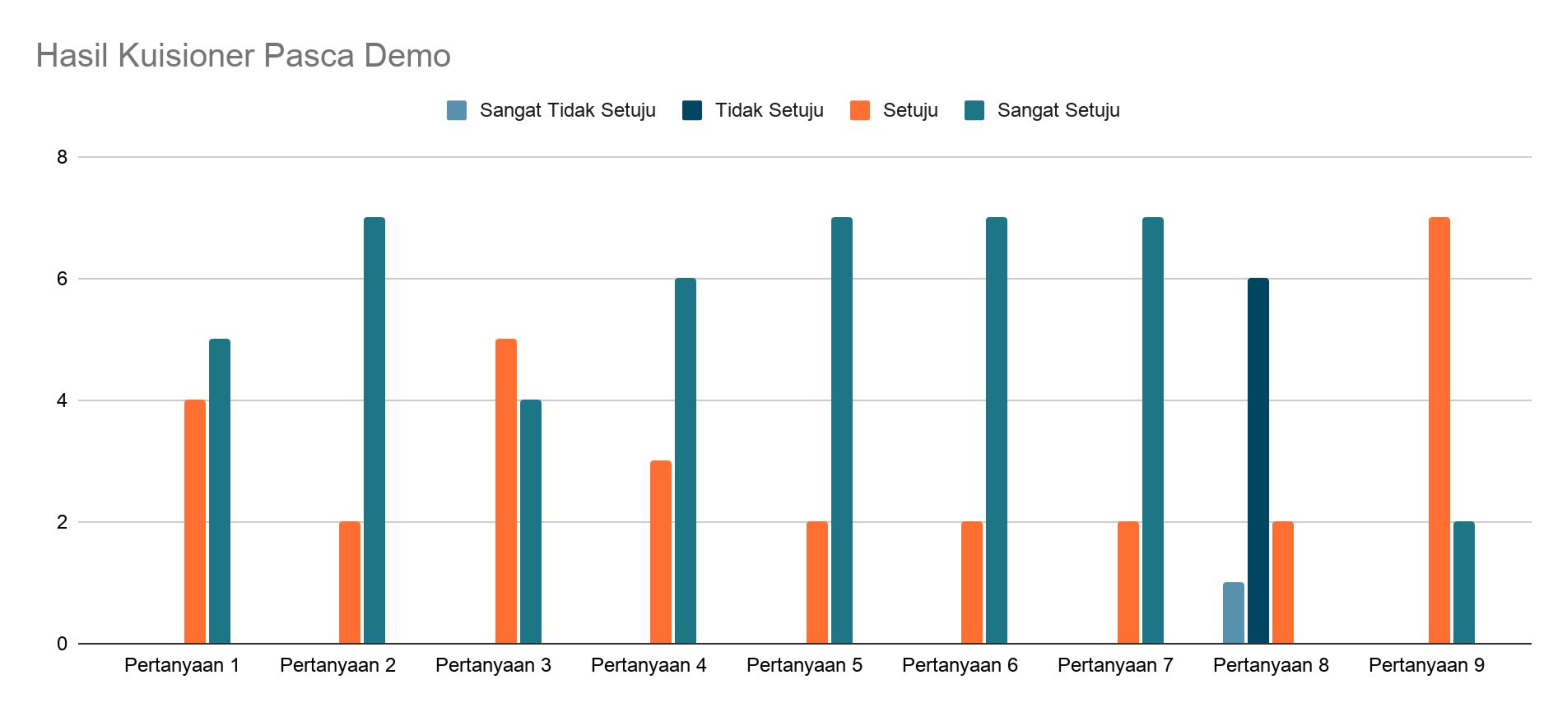
\includegraphics[width=0.75\paperwidth]{Gambar/Hasil Kuisioner.pdf}
        \caption{Hasil kuisioner pasca demo pada pertanyaan berbentuk skala.}
        \label{fig:kuisioner_demo}
    \end{figure}
    
    Hasil kuisioner tersebut dianalisis untuk menilai tingkat kepuasan dalam menggunakan aplikasi. Berdasarkan
    kuisioner yang telah dilakukan, didapatkan rata-rata nilai kepuasan terhadap sistem yang baru dengan
    rincian yang dapat dilihat pada tabel \ref{tab:survey-avg}.
    \begin{table}[]
        \centering
        \begin{tabularx}{\textwidth}{|X|X|}
            \hline
             Parameter & Rata-rata Nilai kepuasan (skala 1 hingga 5)  \\
            \hline
             Pengelolaan data untuk ujian (Nomor 1) &  3.56 \\
            \hline
             Pengiriman berkas jawaban ujian (Nomor 2) &  3.78\\
            \hline
             Pembuatan ujian (Nomor 3) &  3.8 \\
            \hline
             Pengunggahan data untuk ujian (Nomor 4) &  3.67 \\
            \hline
             Pendistribusian informasi layanan dan notifikasi peserta (Nomor 5) &  3.78 \\
            \hline
             Penggunaan Admin Panel (Nomor 6) &  3.78 \\
            \hline
             Migrasi peserta (Nomor 7) &  3.78 \\
            \hline
             Kestabilan aplikasi (Nomor 8) &  2.1 \\
            \hline
             \textbf{Kepuasan secara keseluruhan} (Nomor 9) &  \textbf{3.2} \\
            \hline
        \end{tabularx}
        \caption{Rata-rata nilai kepuasan berdasarkan kuisioner yang telah dilakukan.}
        \label{tab:survey-avg}
    \end{table}

\section{Pengujian Fungsional}
Pengujian fungsional dilakukan dengan bantuan \textit{Unit Testing}. Tes tersebut akan dilakukan
setiap kali kode diunggah ke repositori penyimpanan kode sumber dengan bantuan CI/CD. Tes tersebut
terdiri dari beberapa skenario dan langkah yang menentukan sebuah fitur dapat berjalan sesuai ekspektasi
atau tidak. Tes-tes tersebut terdiri dari
\begin{enumerate}
    \item Otentikasi\\
        Memastikan fitur kelas utama otentikasi dapat berjalan dengan semestinya.\\
        \begin{tabularx}{0.9\textwidth}{|X|X|X|X|X|}
            \hline
            \textit{Test Step} & \textit{Preconditions} & Ekspektasi Hasil & Hasil Didapatkan & Status  \\
            \hline
            Login dengan kata sandi yang salah harus ditolak. & Username benar dan kata sandi salah. & Mengeluarkan Eksepsi & Eksepsi didapatkan & Lolos \\
            \hline
            Login dengan username yang salah harus ditolak. & Username salah dan kata sandi benar. & Mengeluarkan Eksepsi & Eksepsi didapatkan & Lolos \\
            \hline
            Login dengan kredensial yang benar harus diterima. & Username dan kata sandi benar & Kelas mengembalikan nilai \texttt{true} & Kelas mengembalikan nilai \texttt{true} & Lolos \\
            \hline
        \end{tabularx}
        
    \item Ujian tanpa \textit{shift}\\
        Memastikan fungsi yang bertugas untuk memetakan ujian dasar dapat berjalan sesuai ekspektasi.\\
         \begin{tabularx}{0.9\textwidth}{|X|X|X|X|X|}
            \hline
            \textit{Test Step} & \textit{Preconditions} & Ekspektasi Hasil & Hasil Didapatkan & Status  \\
            \hline
            
            \multicolumn{5}{|l|}{\textbf{Ujian yang aktif hanya akan muncul pada saat \textit{flag} \texttt{upcoming} dimatikan.}}\\
            \hline
            Melakukan pemanggilan model dengan \textit{query} \textit{flag} \texttt{upcoming} aktif. &
            Ujian sedang aktif. & Tidak mengeluarkan ujian apapun & Ujian tidak didapatkan & Lolos \\
            \hline
            Melakukan pemanggilan model dengan \textit{query} \textit{flag} \texttt{upcoming} tidak aktif. &
            Ujian sedang aktif. & Mengeluarkan sebuah ujian yang baru saja dibuat & 
            Ujian didapatkan, ujian tersebut sesuai dengan ujian yang dibuat diawal. & Lolos \\
            \hline
            
            \multicolumn{5}{|l|}{\textbf{Ujian yang akan aktif hanya akan didapatkan dengan \textit{flag} \texttt{upcoming} aktif. }}\\
            \hline
            Melakukan pemanggilan model dengan \textit{query} \textit{flag} \texttt{upcoming} aktif. &
            Ujian sedang aktif. & Mengeluarkan sebuah ujian yang baru saja dibuat & 
            Ujian didapatkan, ujian tersebut sesuai dengan ujian yang dibuat diawal. & Lolos \\
            \hline
            Melakukan pemanggilan model dengan \textit{query} \textit{flag} \texttt{upcoming} tidak aktif. &
            Ujian sedang aktif. & Tidak mengeluarkan ujian apapun & Ujian tidak didapatkan & Lolos \\
            \hline
            
             \multicolumn{5}{|l|}{\textbf{Ujian yang telah selesai tidak akan muncul dimanapun.}}\\
            \hline
            Melakukan pemanggilan model dengan \textit{query} \textit{flag} \texttt{upcoming} aktif. &
            Ujian sedang aktif. & Tidak mengeluarkan ujian apapun & Ujian tidak didapatkan & Lolos \\
            \hline
            Melakukan pemanggilan model dengan \textit{query} \textit{flag} \texttt{upcoming} tidak aktif. &
            Ujian sedang aktif. & Tidak mengeluarkan ujian apapun & Ujian tidak didapatkan & Lolos \\
            \hline
        \end{tabularx}
        
    \item Ujian dengan \textit{shift}\\
        Memastikan fungsi yang bertugas untuk memetakan ujian dengan \textit{shift} dapat berjalan sesuai ekspektasi.\\
        
        \begin{tabularx}{0.9\textwidth}{|X|X|X|X|X|}
            \hline
            \textit{Test Step} & \textit{Preconditions} & Ekspektasi Hasil & Hasil Didapatkan & Status  \\
            \hline
            %% CASE 1
            \multicolumn{5}{|p{0.8\textwidth}|}{\textbf{Kedua \textit{shift} akan aktif.}}\\
            \hline
            Melakukan pemanggilan model dengan \textit{query} \textit{flag} \texttt{upcoming} aktif. &
            \textit{Shift} 1 dan 2 akan aktif & Ujian \textit{shift} 1 didapatkan. & Ujian \textit{shift} 1 didapatkan. & Lolos \\
            \hline
            Melakukan pemanggilan model dengan \textit{query} \textit{flag} \texttt{upcoming} tidak aktif. &
            \textit{Shift} 1 dan 2 akan aktif & Tidak ada ujian yang didapatkan. & Tidak ada ujian yang didapatkan. & Lolos \\
            \hline
            
            %% CASE 2
            \multicolumn{5}{|p{0.8\textwidth}|}{\textbf{Ujian pada \textit{shift} 1 aktif dan \textit{shift} 2 akan aktif.}}\\
            \hline
            Melakukan pemanggilan model dengan \textit{query} \textit{flag} \texttt{upcoming} aktif. &
            \textit{Shift} 1 aktif dan \textit{shift} 2 akan aktif & Ujian \textit{shift} 2 didapatkan. & Ujian \textit{shift} 2 didapatkan. & Lolos \\
            \hline
            Melakukan pemanggilan model dengan \textit{query} \textit{flag} \texttt{upcoming} tidak aktif. &
            \textit{Shift} 1 aktif dan \textit{shift} 2 akan aktif & Ujian \textit{shift} 1 didapatkan. & Ujian \textit{shift} 1 didapatkan. & Lolos \\
            \hline
            
            %% CASE 3
            \multicolumn{5}{|p{0.8\textwidth}|}{\textbf{Ujian pada \textit{shift} 1 selesai dan \textit{shift} 2 akan dimulai.}}\\
            \hline
            Melakukan pemanggilan model dengan \textit{query} \textit{flag} \texttt{upcoming} aktif. &
            \textit{Shift} 1 selesai dan \textit{shift} 2 akan aktif & Ujian \textit{shift} 2 didapatkan. & Ujian \textit{shift} 2 didapatkan. & Lolos \\
            \hline
            Melakukan pemanggilan model dengan \textit{query} \textit{flag} \texttt{upcoming} tidak aktif. &
            \textit{Shift} 1 selesai dan \textit{shift} 2 akan aktif & Tidak ada ujian yang didapatkan. & Tidak ada ujian yang didapatkan. & Lolos \\
            \hline
            
            %% CASE 4
            \multicolumn{5}{|p{0.8\textwidth}|}{\textbf{Ujian pada \textit{shift} 1 selesai dan \textit{shift} 2 sedang aktif.}}\\
            \hline
            Melakukan pemanggilan model dengan \textit{query} \textit{flag} \texttt{upcoming} aktif. &
            \textit{Shift} 1 selesai dan \textit{shift} 2 aktif & Tidak ada ujian yang didapatkan. & Tidak ada ujian yang didapatkan. & Lolos \\
            \hline
            Melakukan pemanggilan model dengan \textit{query} \textit{flag} \texttt{upcoming} tidak aktif. &
            \textit{Shift} 1 selesai dan \textit{shift} 2 aktif & Ujian \textit{shift} 2 didapatkan. & Ujian \textit{shift} 2 didapatkan. & Lolos \\
            \hline
        \end{tabularx}\\
        \begin{tabularx}{0.9\textwidth}{|X|X|X|X|X|}
            \hline
            \textit{Test Step} & \textit{Preconditions} & Ekspektasi Hasil & Hasil Didapatkan & Status  \\
            \hline
            %% CASE 5
            \multicolumn{5}{|p{0.8\textwidth}|}{\textbf{Ujian pada \textit{shift} 1 dan 2 selesai.}}\\
            \hline
            Melakukan pemanggilan model dengan \textit{query} \textit{flag} \texttt{upcoming} aktif. &
            \textit{Shift} 1 selesai dan \textit{shift} 2 selesai & Tidak ada ujian yang didapatkan. & Tidak ada ujian yang didapatkan. & Lolos \\
            \hline
            Melakukan pemanggilan model dengan \textit{query} \textit{flag} \texttt{upcoming} tidak aktif. &
            \textit{Shift} 1 selesai dan \textit{shift} 2 selesai & Tidak ada ujian yang didapatkan. & Tidak ada ujian yang didapatkan. & Lolos \\
            \hline
        \end{tabularx}
        
\end{enumerate}


